\chapter{Algoritmo de sincronización y control de formaciones}\label{cap:algoritmo}
El algoritmo de sincronización y control de formaciones funciona con dos programas principales. El primero es el algoritmo de sincronización y control centralizado llamado ``supervisor'' y el segundo es el algoritmo de control de uniciclo para los agentes. En este capítulo se explicará el funcionamiento de cada uno y la lógica detrás de ellos para cumplir con las tareas de formación, evasión de colisiones y movilización hacia un objetivo.

\section{Programa del supervisor}
El programa del supervisor tiene como tarea coordinar a los agentes, realizar procesamiento de datos y generar trayectorias para movilizarlos hacia un objetivo, evadiendo colisiones entre ellos y con los obstáculos. Para esto, el algoritmo cuenta con diferentes segmentos.

\subsection{Adquisición de posiciones}
La primera parte del algoritmo consiste en la toma de las posiciones actuales $X$ y $Y$ de los agentes, obstáculos y el objetivo. 

\subsection{Cálculo de velocidades de agentes}
Luego, se calculan las velocidades de los agentes para desplazarlos tanto hacia su posición en la formación como hacia el objetivo de interés. Este cálculo se realiza por medio de la ecuación de consenso con un factor de peso $\omega$ el cual depende de las ecuaciones de tensión y evasión de obstáculos. 

\subsection{Evasión de obstáculos y colisiones}
Seguido a esto, se implementa la evasión de obstáculos y colisiones, comparando la posición actual de cada agente con la de sus vecinos y los obstáculos.

\subsection{Control proporcional}
El siguiente segmento implementa el control proporcional de la Ecuación (\ref{eq:controlador_proporcional}) para movilizar a los agentes hacia un punto de interés.

\begin{equation}
	v_{n+1} = v_n + k(x_{objetivo} - x_{agente})
	\label{eq:controlador_proporcional}
\end{equation}

Donde $v$ es la velocidad del agente y $k$ es la ganancia o constante de proporcionalidad que multiplica a la distancia entre el punto de interés y la posición del agente evaluado. Una vez se obtienen las componentes de velocidad en $X$ y $Y$, se calcula la norma de velocidad, la cual se utiliza para la toma de decisiones dentro del algoritmo.

En la Figura \ref{fig:diagrama_supervisor} se muestra el diagrama de flujo que representa el programa del supervisor.

\section{Programa de los agentes}
El programa del los agentes recibe las velocidades calculadas por el supervisor. Luego, se encarga de convertirlas en sus componentes lineal y angular para calcular la velocidad de cada rueda de los Pololu 3Pi+, utilizando el modelo del uniciclo. Este programa es individual para cada agente y solo procesa los datos correspondientes a su propio funcionamiento.

En la Figura \ref{fig:diagrama_agentes} se muestra el diagrama de flujo que representa el control de los agentes.

\section{Funcionamiento del algoritmo}
El algoritmo consta de las siguientes etapas para su ejecución:
\begin{itemize}
	\item Etapa 0: los agentes se movilizan hacia sus posiciones iniciales para iniciar el experimento.
	\item Etapa 1: comienza el acercamiento de agentes hasta que la norma de velocidad esté por debajo de un valor seleccionado.
	\item Etapa 2: los agentes se colocan en sus posiciones de la formación hasta que el error cuadrático medio entre la formación actual y la deseada esté por debajo de un valor seleccionado.
	\item Etapa 3: el líder se mueve hacia el objetivo y los agentes de la formación lo siguen.
\end{itemize}

Cabe mencionar que durante toda la ejecución del algoritmo, se realiza la evasión de obstáculos y colisiones.

\begin{figure}[H]
	\centering
	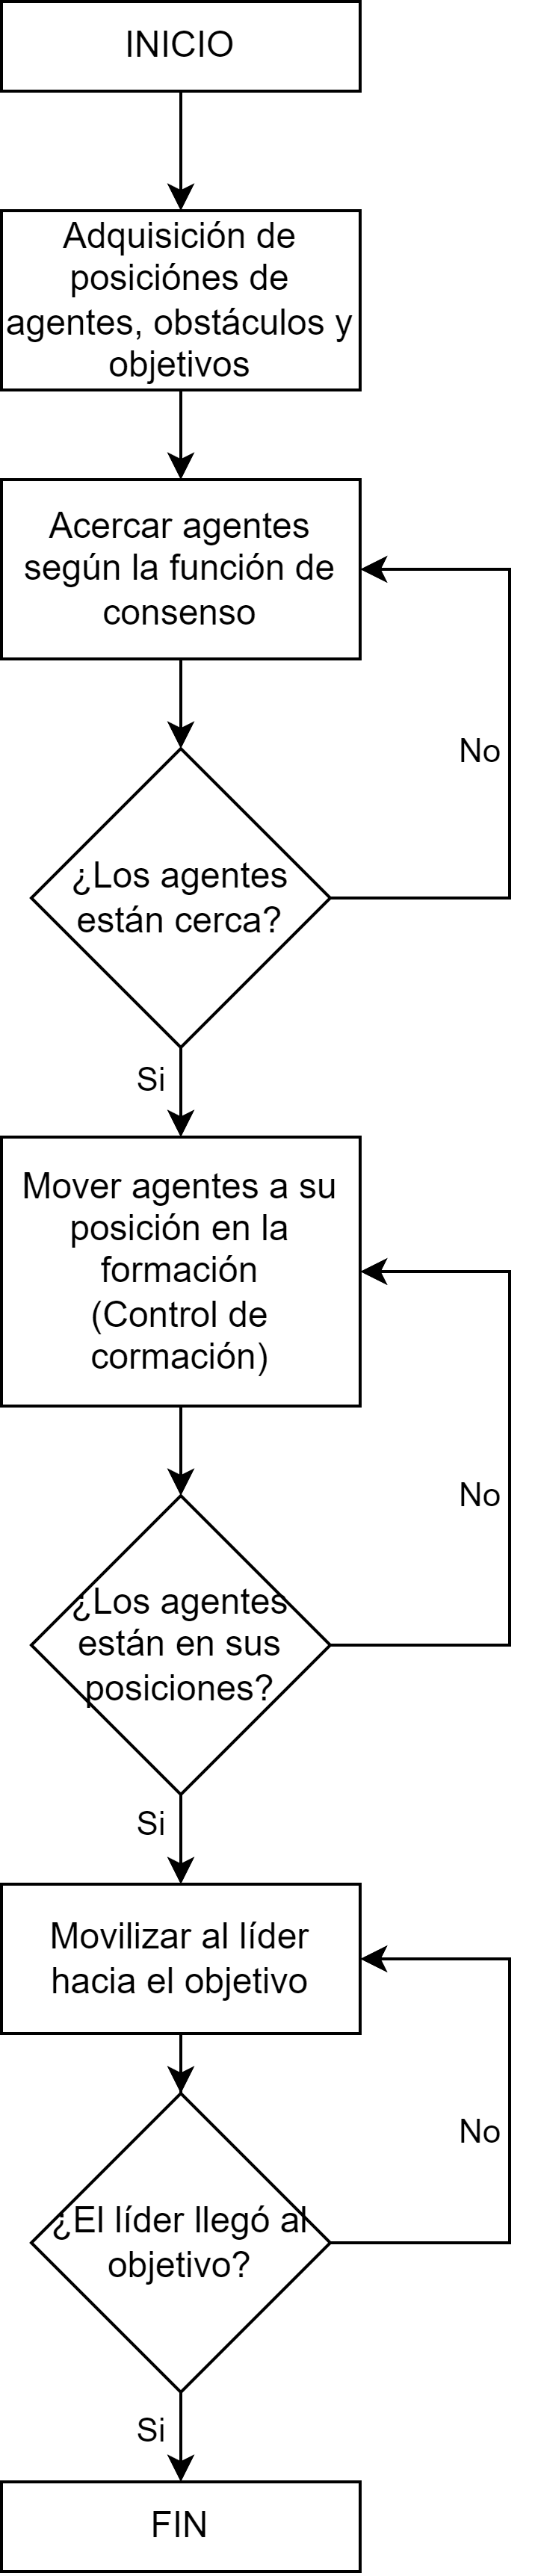
\includegraphics[width=0.20\textwidth]{optimizacion/diagrama_supervisor.png}
	\caption{Diagrama de flujo para el supervisor.}
	\label{fig:diagrama_supervisor}
\end{figure}

\begin{figure}[H]
	\centering
	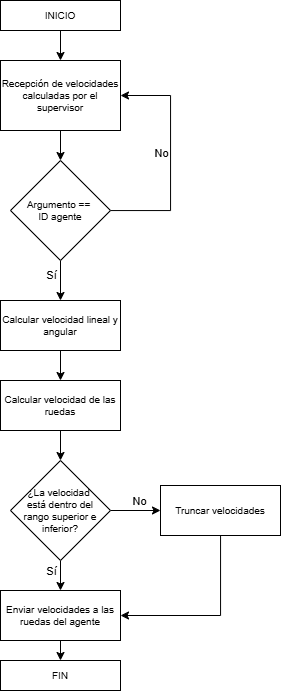
\includegraphics[width=0.45\textwidth]{optimizacion/diagrama_agentes.png}
	\caption{Diagrama de flujo para el programa de los agentes.}
	\label{fig:diagrama_agentes}
\end{figure}


\chapter{Verificación de funcionalidad del algoritmo desarrollado en fases previas}\label{cap:restauracion}

La implementación en físico del algoritmo de sincronización y control de formaciones realizada por José Alejandro Rodríguez \cite{RodriguezJA_2023_tesis}, se llevó a cabo en Webots, versión R2023b, la misma que se utiliza en la fase actual del proyecto. Para el desarrollo del controlador del supervisor y los agentes, se optó por utilizar Python 3.10 como lenguaje de programación ya que es una de las versiones más recientes y es la misma empleada en la fase anterior. Asimismo, el servidor del Robotat ha experimentado cambios en su infraestructura, lo que ha afectado la conexión con los Pololu 3Pi+. Como resultado, ha sido necesario un reajuste de parámetros y configuraciones en el algoritmo para adaptarlo a las nuevas condiciones de conexión.

En este capítulo se detallan las modificaciones necesarias para ejecutar el algoritmo y garantizar su correcto funcionamiento tanto en simulaciones de Webots como en un entorno físico en el Robotat. Además, se valida la naturaleza del algoritmo en escenarios con obstáculos móviles.


\section{Réplica de simulaciones de Webots}
El primer paso de la verificación, fue recrear algunas simulaciones en Webots. Para esto, fue necesario instalar las siguientes librerías que no se encuentran dentro de las librerías estándar de Python:

\begin{itemize}
	\item Keyboard - versión 0.13.5
	\item NumPy - versión 1.23.2
\end{itemize}

Luego, se realizó la prueba del código para el controlador del supervisor y los agentes incluyendo sus respectivas funciones:
\begin{itemize}
	\item Supervisor: Supervisor\_simulacion\_y\_fisico\_v4.py
	\item Agentes: pruebaMatrizDifeomorfismo.py
	\item Funciones algoritmo: funciones.py, funVel.py
\end{itemize} 

\subsection{Comunicación entre supervisor y agentes}
Al ejecutar la primera simulación, se encontró que dos agentes permanecían inmóviles durante la ejecución del programa, tal como se muestra en la Figura \ref{fig:delaygpu}.

\begin{figure}[H]
	\centering
	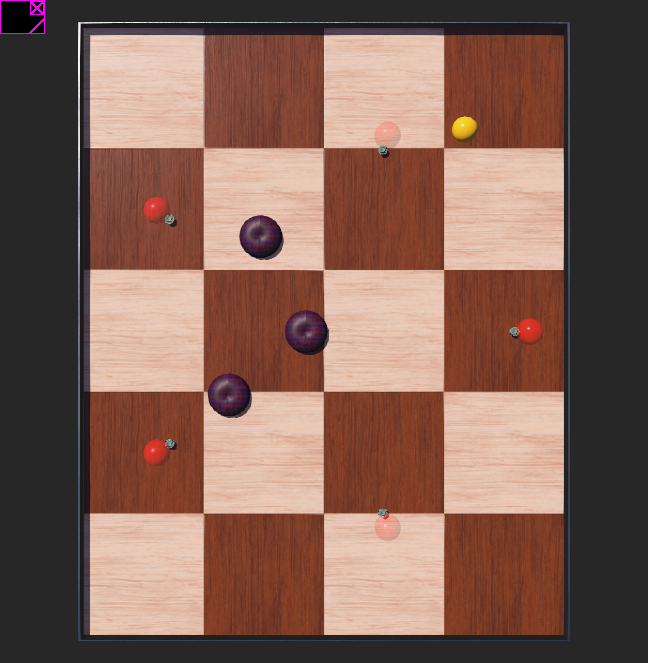
\includegraphics[width=0.30\textwidth]{replicar_webots/delaygpu_v2_1.png}
	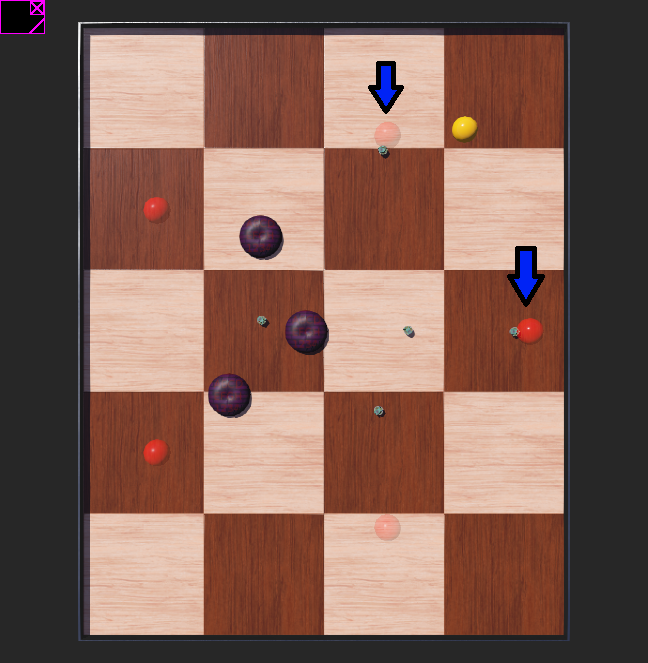
\includegraphics[width=0.30\textwidth]{replicar_webots/delaygpu_v2_2.png}
	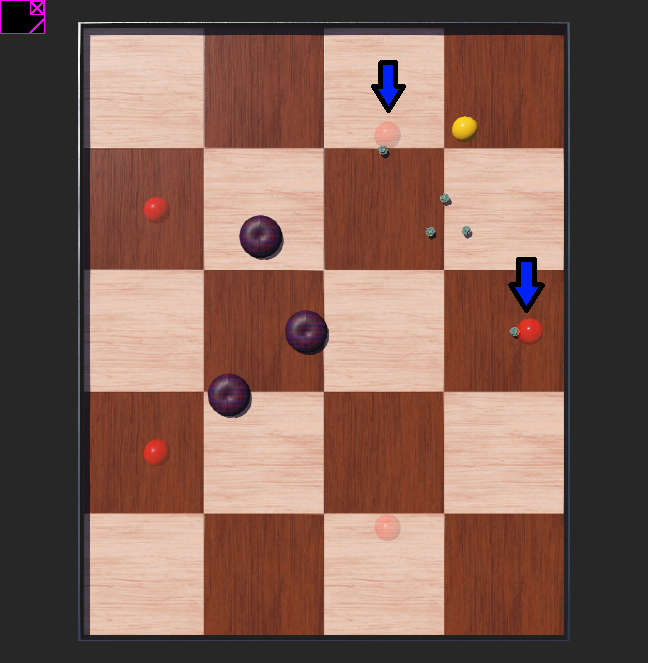
\includegraphics[width=0.30\textwidth]{replicar_webots/delaygpu_v2_3.png}
	\caption{Ejecución de la primera simulación en Webots 2023b.}
	\label{fig:delaygpu}
\end{figure}

Esto se debe a que actualmente se está utilizando una computadora con mayor capacidad de procesamiento que la utilizada en la fase anterior y esto se ve reflejado en la velocidad de ejecución de los programas. 

Dado que la comunicación entre el supervisor y los agentes se realiza por medio de una memoria compartida, al tener mayor velocidad de procesamiento, el controlador de los dos primeros agentes se ejecuta antes de que el espacio de memoria compartida se haya inicializado correctamente. Para solucionar esto, en el programa de los agentes, se agregó un tiempo de espera de 3 segundos antes de inicializar y acceder a la memoria compartida. Esto permite que se inicialice correctamente en el programa del supervisor.

\subsection{Prueba del algoritmo con simulaciones basadas en escenarios previos}
Una vez solucionado el problema de comunicación, se realizó las primeras simulaciones para replicar algunos de los escenarios realizados en la fase previa y comprobar el funcionamiento correcto del algoritmo. 

El código del supervisor ya cuenta con un modo de simulación en el que se ejecuta el algoritmo basado en condiciones iniciales tomadas de un escenario físico. Para esto, se debe cargar un archivo .npz que cuenta con la información necesaria para configurar la simulación según el escenario real en que se ejecutó el algoritmo.

\subsubsection{Primer escenario}
Para la primera simulación, se utilizó el archivo ``finaltrial\_6A\_AAA\_f\_1.npz'' que consiste en la siguiente configuración:

\begin{itemize}
	\item Cantidad de agentes: 6
	\item Posición inicial de agentes: línea
	\item Obstáculos: ninguno
	\item Objetivo: ubicado en la esquina
\end{itemize}

En la Figura \ref{fig:primera_simulacion}, las imágenes en el orden de izquierda a derecha y luego de arriba hacia abajo muestran la secuencia de ejecución del algoritmo.

\begin{figure}[H]
	\centering
	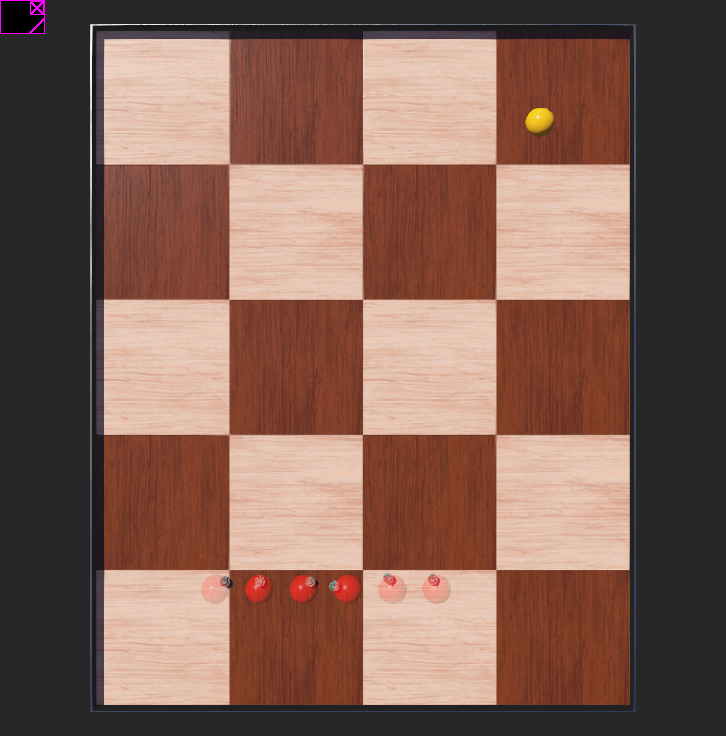
\includegraphics[width=0.40\textwidth]{replicar_webots/sim1_p1.png}
	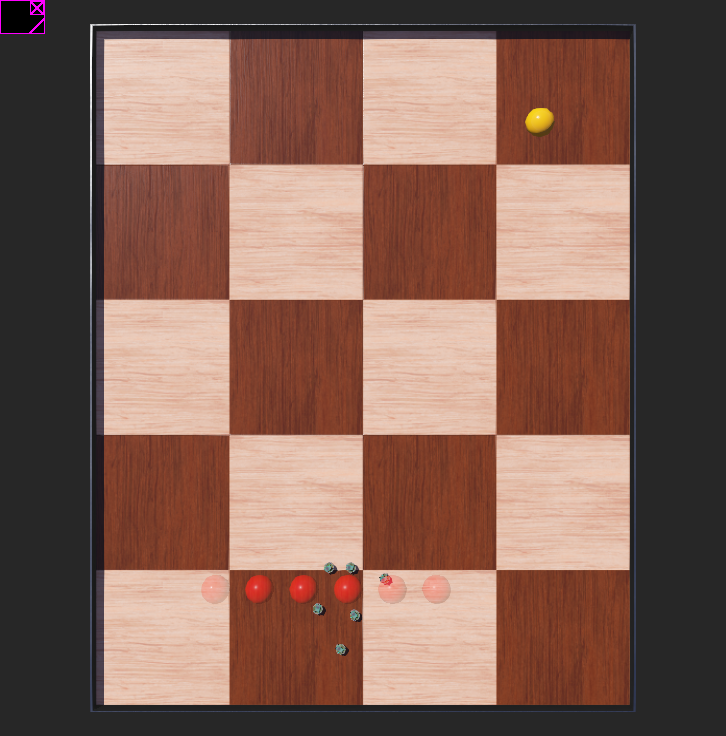
\includegraphics[width=0.40\textwidth]{replicar_webots/sim1_p2.png}
	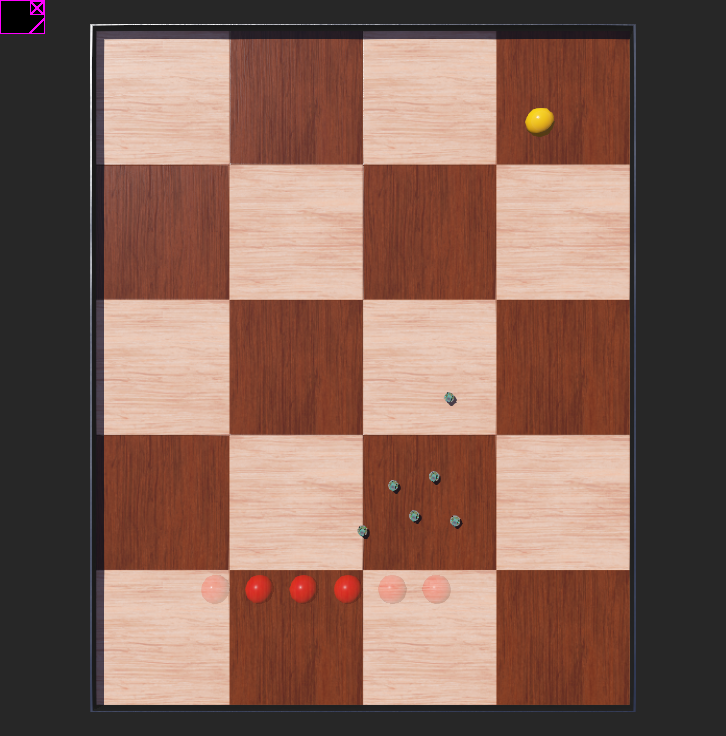
\includegraphics[width=0.40\textwidth]{replicar_webots/sim1_p3.png}
	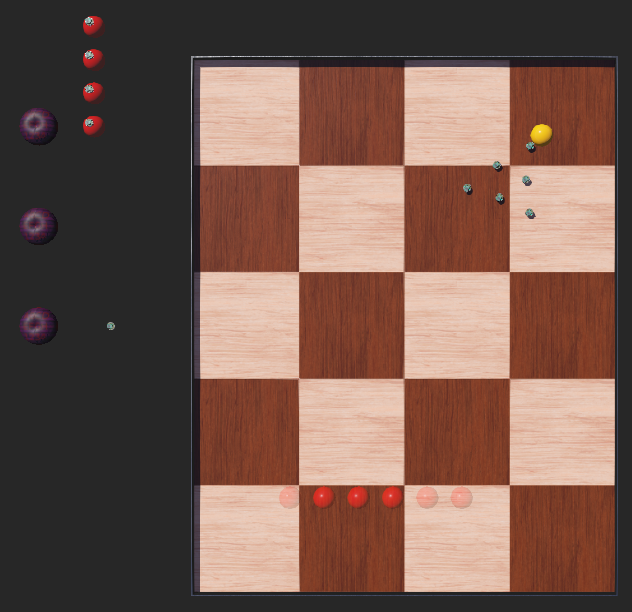
\includegraphics[width=0.40\textwidth]{replicar_webots/sim1_p4.png}
	\caption{Ejecución del algoritmo en la primera simulación}
	\label{fig:primera_simulacion}
\end{figure}

\subsubsection{Segundo escenario}
Para la segunda simulación, se utilizó el archivo ``finaltrial\_6A\_AB1B\_f\_2.npz'' que consiste en la siguiente configuración:

\begin{itemize}
	\item Cantidad de agentes: 6
	\item Posición inicial de agentes: línea
	\item Obstáculos: ubicados en el centro
	\item Objetivo: ubicado en el centro
\end{itemize}

En la Figura \ref{fig:segunda_simulacion}, las imágenes en el orden de izquierda a derecha y luego de arriba hacia abajo muestran la secuencia de ejecución del algoritmo.

\begin{figure}[H]
	\centering
	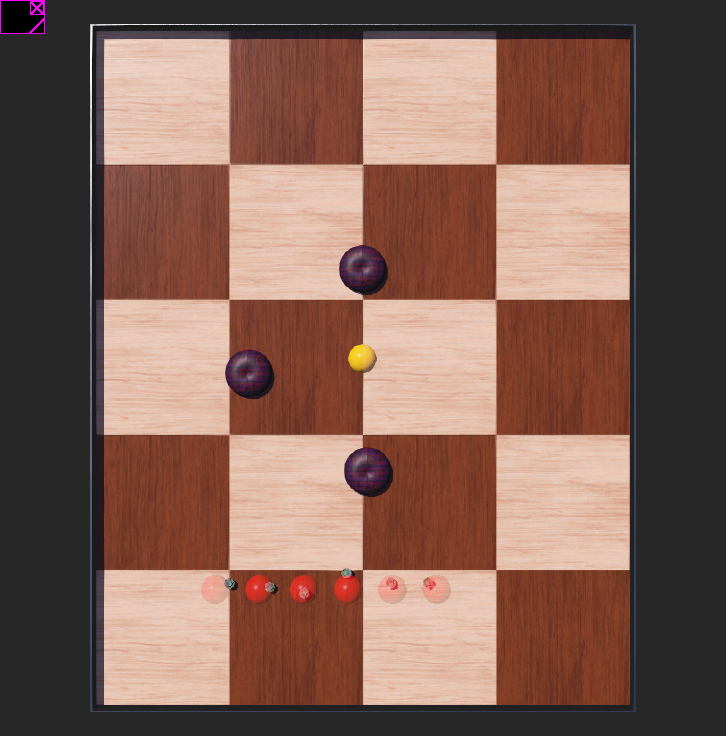
\includegraphics[width=0.45\textwidth]{replicar_webots/sim2_p1.png}
	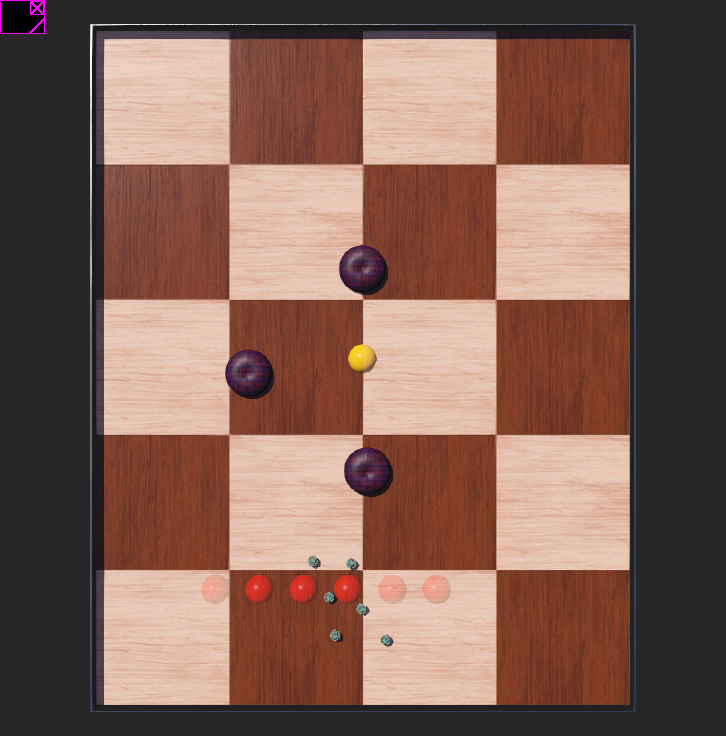
\includegraphics[width=0.45\textwidth]{replicar_webots/sim2_p2.png}
	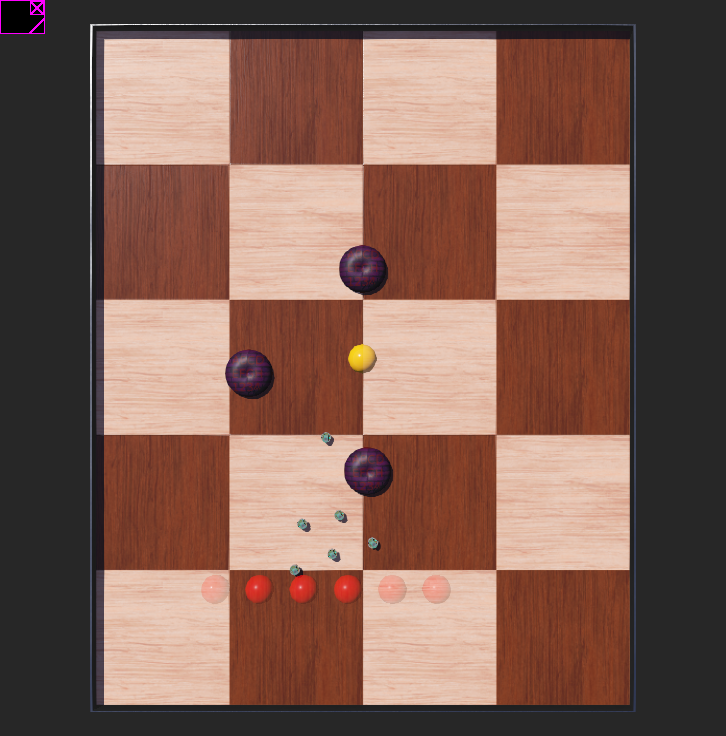
\includegraphics[width=0.45\textwidth]{replicar_webots/sim2_p3.png}
	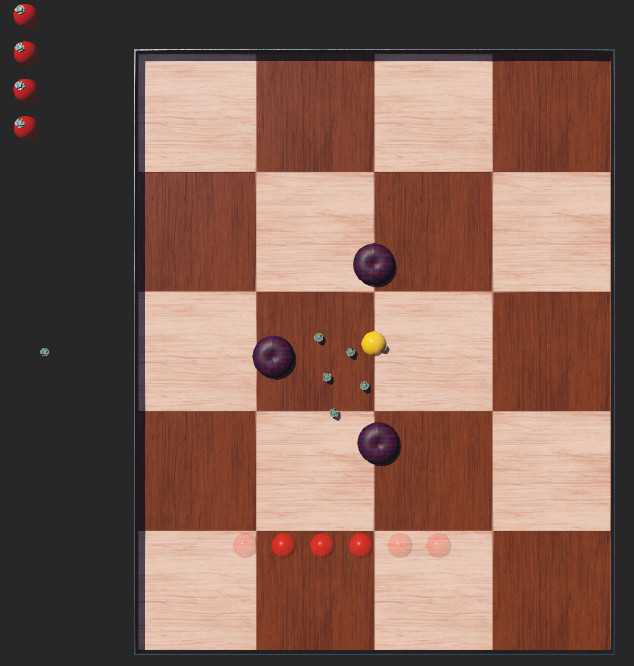
\includegraphics[width=0.45\textwidth]{replicar_webots/sim2_p4.png}
	\caption{Ejecución del algoritmo en la segunda simulación}
	\label{fig:segunda_simulacion}
\end{figure}

\subsubsection{Tercer escenario}
Para la tercera simulación, se utilizó el archivo ``finaltrial\_6A\_BCA\_f\_1.npz'' que consiste en la siguiente configuración:

\begin{itemize}
	\item Cantidad de agentes: 6
	\item Posición inicial de agentes: círculo
	\item Obstáculos: ubicados en posiciones aleatorias
	\item Objetivo: ubicado en la esquina
\end{itemize}

En la Figura \ref{fig:tercera_simulacion}, las imágenes en el orden de izquierda a derecha y luego de arriba hacia abajo muestran la secuencia de ejecución del algoritmo.

\begin{figure}[H]
	\centering
	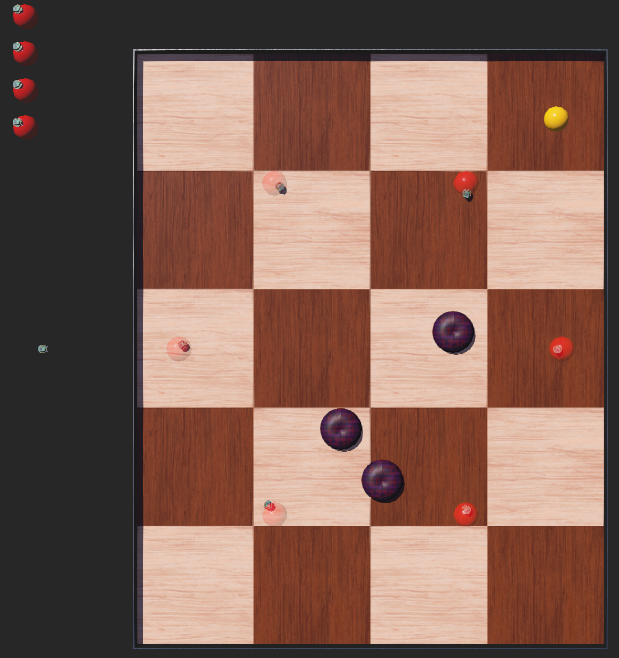
\includegraphics[width=0.45\textwidth]{replicar_webots/sim3_p1.png}
	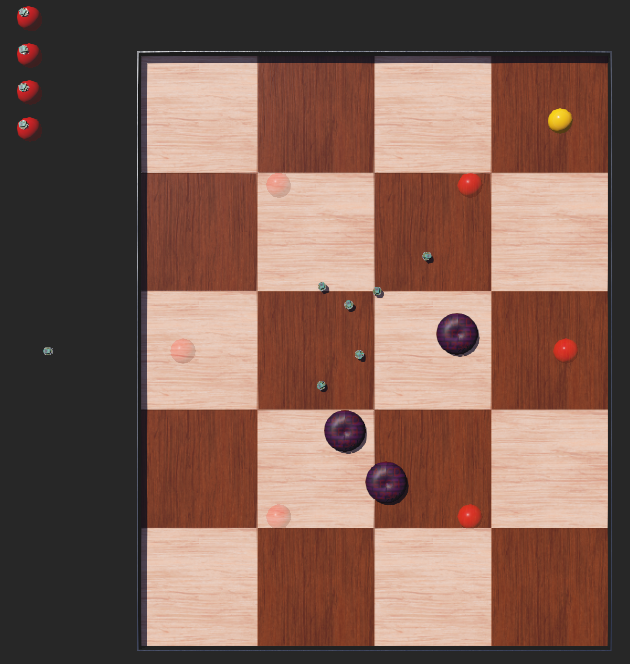
\includegraphics[width=0.45\textwidth]{replicar_webots/sim3_p2.png}
	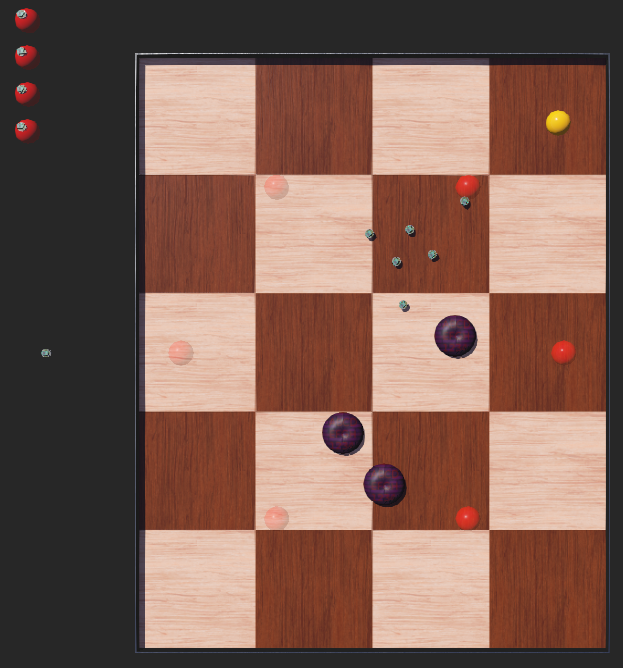
\includegraphics[width=0.45\textwidth]{replicar_webots/sim3_p3.png}
	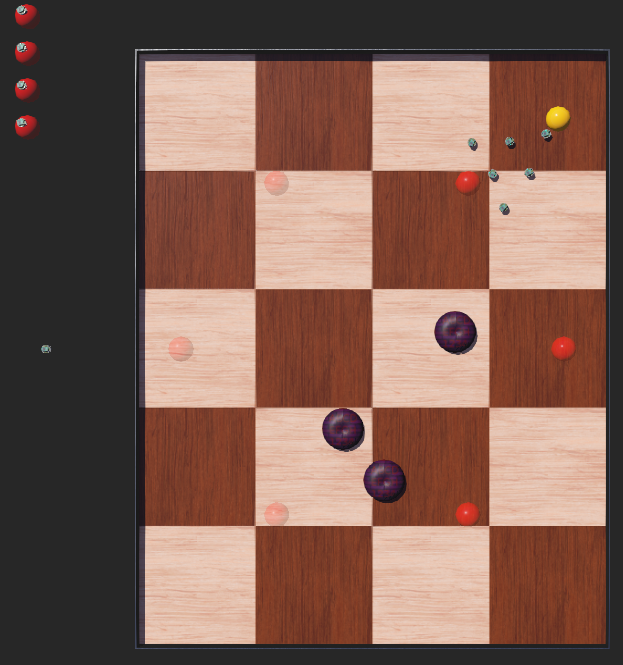
\includegraphics[width=0.45\textwidth]{replicar_webots/sim3_p4.png}
	\caption{Ejecución del algoritmo en la tercera simulación}
	\label{fig:tercera_simulacion}
\end{figure}

\section{Réplica del funcionamiento del algoritmo en el Robotat}
Una vez que el algoritmo funcionó correctamente en Webots, el siguiente paso fue verificar que se ejecutara correctamente en el Robotat.

\subsection{Pruebas de conexión con el Pololu 3Pi+ y el Robotat}
 Primero, se realizaron pruebas de conexión con el Robotat y los Pololu 3Pi+ utilizando las funciones creadas en Python durante la fase previa:
 
\begin{itemize}
	\item robotat\_connect
	\item robotat\_disconnect
	\item robotat\_get\_pose
	\item robotat\_3pi\_connect
	\item robotat\_3pi\_disconnect
	\item robotat\_3pi\_set\_wheel\_velocities
	\item robotat\_3pi\_force\_stop
\end{itemize}

Al intentar conectar con los agentes Pololu 3Pi+ se tuvo el error mostrado en la Figura \ref{fig:error_conexion}. Este se debe a que hubo un cambio en los puertos de conexión con el ESP$32$ de los agentes. Anteriormente la conexión se realizaba en el puerto $8888$ y actualmente se realiza en el puerto $9090$. Al actualizar este parámetro dentro de la función ``robotat\_3pi\_connect'' en del archivo ``funciones\_conjunto\_3pi.py'', se obtuvo la conexión exitosa con el agente.

\begin{figure}[H]
	\centering
	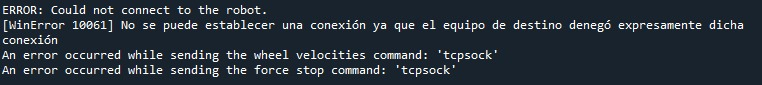
\includegraphics[width=0.8\textwidth]{replicar_fisico_pruebas/error_conexion.png}
	\caption{Error de conexión con Pololu 3Pi+.}
	\label{fig:error_conexion}
\end{figure}

\subsection{Calibración de marcadores}
El siguiente paso fue realizar una nueva calibración de los marcadores del OptiTrack para obtener el desfase del ángulo orientación (\textit{bearing}) de cada marcador. Estos desfases son diferentes para cada uno y se producen por la forma en que el OptiTrack los identifica según la posición de sus esferas reflectivas.

En la fase anterior, se realizó una calibración con los marcadores del $1$ al $15$, sin embargo, se agregaron nuevos marcadores al Robotat y ahora se cuenta con $22$ de ellos. Actualmente, los marcadores $1$ y $9$ están inhabilitados ya que serán utilizados en otros proyectos de graduación. Por tanto, ahora se tienen disponibles los marcadores de la Figura \ref{fig:marcadores_disponibles}. 

\begin{figure}[H]
	\centering
	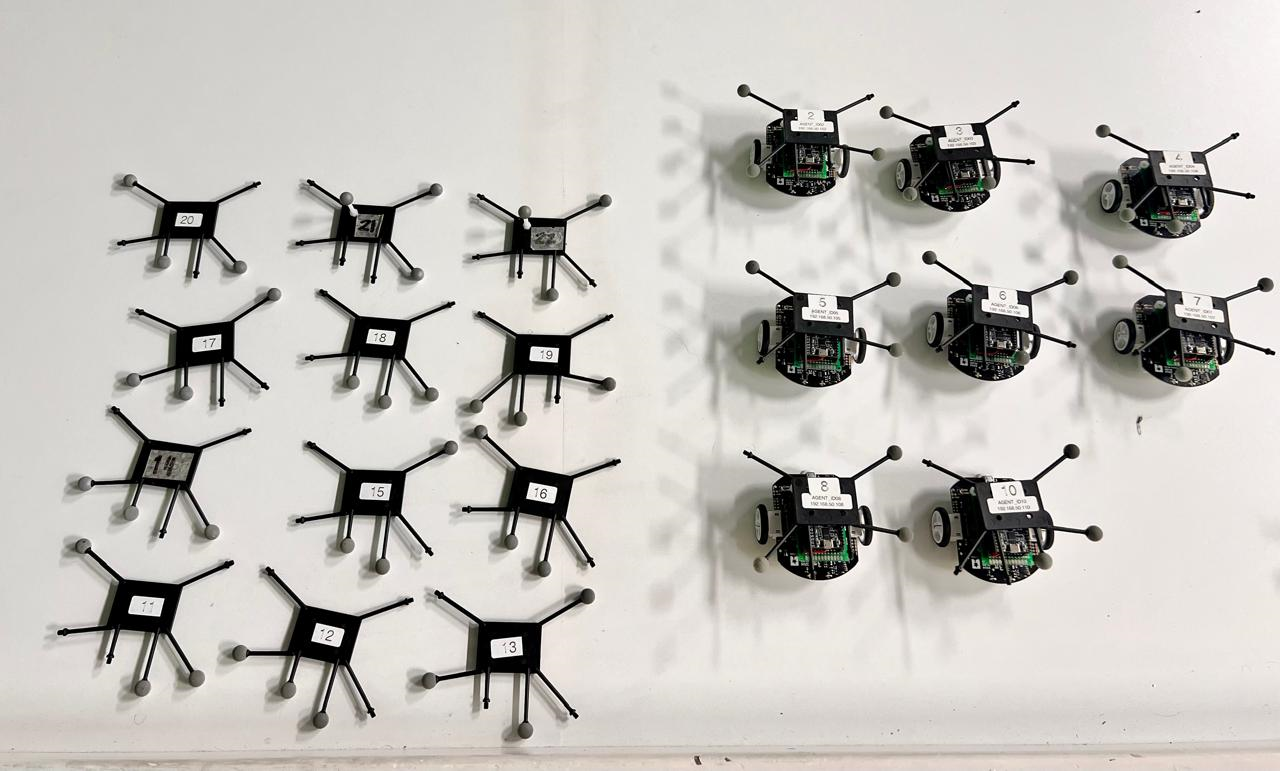
\includegraphics[width=0.8\textwidth]{replicar_fisico_pruebas/marcadores_disponibles.png}
	\caption{Marcadores del OptiTrack disponibles para su uso.}
	\label{fig:marcadores_disponibles}
\end{figure}

Para corregir el desfase de cada marcador, primero se obtiene la orientación con ángulos de Euler en la secuencia $zyx$, luego, al primer ángulo que representa la rotación respecto al eje $z$ se le resta el desfase obtenido $\theta_z$. Para realizar la calibración, se colocaron todos los marcadores disponibles de la Figura \ref{fig:marcadores_disponibles} con la misma orientación sobre el eje $y$ de la mesa de pruebas del Robotat tal como se observa en la Figura \ref{fig:marcadores_calibracion}.

\begin{figure}[H]
	\centering
	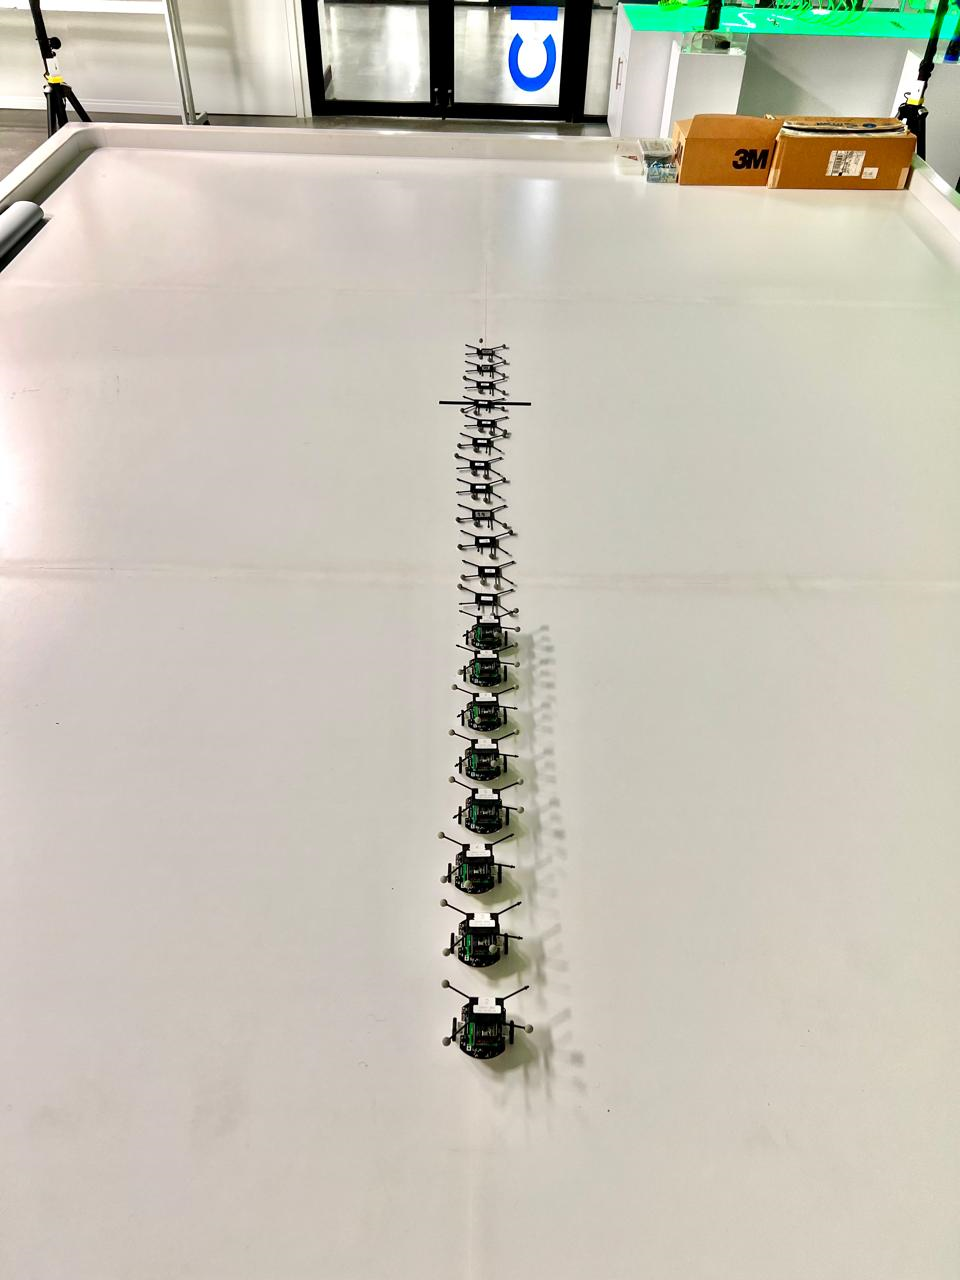
\includegraphics[width=0.6\textwidth]{replicar_fisico_pruebas/marcadores_ejey.png}
	\caption{Marcadores alineados sobre el eje $y$ de la mesa de pruebas del Robotat.}
	\label{fig:marcadores_calibracion}
\end{figure}

Al obtener la pose de cada marcador, se realizó la conversión a ángulos de Euler en la secuencia $zyx$ y se obtuvo los ángulos de desfase para cada marcador. En el cuadro \ref{cuadro:desfases_finales} se presentan los desfases obtenidos en la fase previa, los desfases obtenidos en la fase actual y los desfases finales utilizados para cada uno de los marcadores del $1$ al $22$. 

Dado que los desfases actuales son similares a los obtenidos en la fase previa, se decidió utilizar los desfases anteriores para los marcadores $1$ y $9$ faltantes en la calibración actual. Por último, los desfases de los marcadores del $1$ al $22$ finales se guardaron en un archivo .npy llamado ``nueva\_calibracion\_markers\_1\_al\_22.npy'' para aplicarlos luego de obtener la pose de cada marcador en el algoritmo y así tener siempre un ángulo respecto del eje $z$ igual a cero ($\theta_z$ = 0).

\begin{table}[H]
	\centering
	\begin{tabular}{|c|rrr|}
		\hline
		\multirow{2}{*}{\textbf{Marcador}} & \multicolumn{3}{c|}{\textbf{Desfase   $\theta_z$ en grados}}                                                                            \\ \cline{2-4} 
		& \multicolumn{1}{c|}{\textbf{Fase previa}} & \multicolumn{1}{c|}{\textbf{Fase actual}} & \multicolumn{1}{c|}{\textbf{Combinado}} \\ \hline
		1                                  & \multicolumn{1}{r|}{91.9947}              & \multicolumn{1}{r|}{N/A}                  & 91.9947                                 \\ \hline
		2                                  & \multicolumn{1}{r|}{-46.8146}             & \multicolumn{1}{r|}{-47.2747}             & -47.2747                                \\ \hline
		3                                  & \multicolumn{1}{r|}{-92.3905}             & \multicolumn{1}{r|}{-90.3228}             & -90.3228                                \\ \hline
		4                                  & \multicolumn{1}{r|}{-138.2067}            & \multicolumn{1}{r|}{-135.7891}            & -135.7891                               \\ \hline
		5                                  & \multicolumn{1}{r|}{176.3752}             & \multicolumn{1}{r|}{179.3715}             & 179.3715                                \\ \hline
		6                                  & \multicolumn{1}{r|}{-144.1822}            & \multicolumn{1}{r|}{-141.0275}            & -141.0275                               \\ \hline
		7                                  & \multicolumn{1}{r|}{-176.3193}            & \multicolumn{1}{r|}{-175.0542}            & -175.0542                               \\ \hline
		8                                  & \multicolumn{1}{r|}{-79.9525}             & \multicolumn{1}{r|}{-78.1154}             & -78.1154                                \\ \hline
		9                                  & \multicolumn{1}{r|}{-9.8762}              & \multicolumn{1}{r|}{N/A}                  & -9.8762                                 \\ \hline
		10                                 & \multicolumn{1}{r|}{139.3579}             & \multicolumn{1}{r|}{143.2079}             & 143.2079                                \\ \hline
		11                                 & \multicolumn{1}{r|}{111.9328}             & \multicolumn{1}{r|}{111.0833}             & 111.0833                                \\ \hline
		12                                 & \multicolumn{1}{r|}{167.5761}             & \multicolumn{1}{r|}{166.1718}             & 166.1718                                \\ \hline
		13                                 & \multicolumn{1}{r|}{-128.0709}            & \multicolumn{1}{r|}{-127.3112}            & -127.3112                               \\ \hline
		14                                 & \multicolumn{1}{r|}{-111.1404}            & \multicolumn{1}{r|}{-109.4993}            & -109.4993                               \\ \hline
		15                                 & \multicolumn{1}{r|}{-43.4112}             & \multicolumn{1}{r|}{-40.7394}             & -40.7394                                \\ \hline
		16                                 & \multicolumn{1}{r|}{N/A}                  & \multicolumn{1}{r|}{-104.1691}            & -104.1691                               \\ \hline
		17                                 & \multicolumn{1}{r|}{N/A}                  & \multicolumn{1}{r|}{-121.1928}            & -121.1928                               \\ \hline
		18                                 & \multicolumn{1}{r|}{N/A}                  & \multicolumn{1}{r|}{-92.4812}             & -92.4812                                \\ \hline
		19                                 & \multicolumn{1}{r|}{N/A}                  & \multicolumn{1}{r|}{4.2981}               & 4.2981                                  \\ \hline
		20                                 & \multicolumn{1}{r|}{N/A}                  & \multicolumn{1}{r|}{-133.2161}            & -133.2161                               \\ \hline
		21                                 & \multicolumn{1}{r|}{N/A}                  & \multicolumn{1}{r|}{-112.0477}            & -112.0477                               \\ \hline
		22                                 & \multicolumn{1}{r|}{N/A}                  & \multicolumn{1}{r|}{-15.2847}             & -15.2847                                \\ \hline
	\end{tabular}
	\caption{Desfases para la calibración de marcadores del $1$ al $22$.}
	\label{cuadro:desfases_finales}
\end{table}

\subsection{Selección de marcadores a utilizar}
Una vez guardada la calibración de marcadores, se realizaron pruebas en el Robotat para ejecutar el algoritmo de sincronización y control de formaciones. Sin embargo, el primer problema que se identificó fue que al menos un agente siempre permanecía inmóvil. En la Figura \ref{fig:agente_inmovil} se observa la ejecución del algoritmo donde únicamente se mueve un agente de los dos utilizados.

\begin{figure}[H]
	\centering
	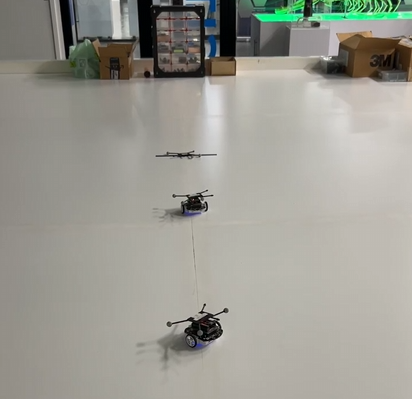
\includegraphics[width=0.45\textwidth]{replicar_fisico_pruebas/agente_inmovil_p1.png}
	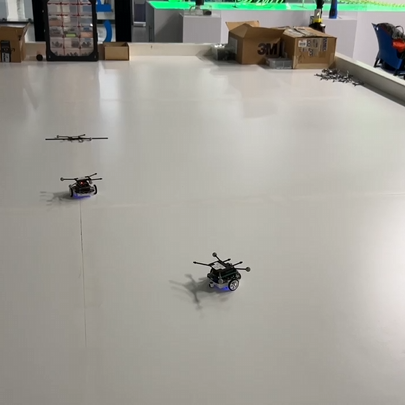
\includegraphics[width=0.45\textwidth]{replicar_fisico_pruebas/agente_inmovil_p2.png}
	\caption{Problema de funcionamiento en físico, agentes permanecen inmóviles.}
	\label{fig:agente_inmovil}
\end{figure}

Anteriormente, para obtener las poses de los marcadores se utilizaba una lista predeterminada con los valores enteros del $1$ al $12$ en orden ascendente que serían los marcadores a utilizar. Sin embargo esto ocasionaba diferentes problemas.

Para obtener las poses de los marcadores se utiliza la función ``robotat\_get\_pose'', esta recibe como argumentos el objeto TCP y los números de marcadores. Al tener una lista predeterminada de valores, siempre se está solicitando la pose de los $12$ marcadores aunque no todos estén en uso, resultando en una solicitud de datos innecesaria para el servidor. Además, dado que durante el desarrollo de este trabajo no se tienen disponibles los marcadores $1$ y $9$, se excede el tiempo de espera (\textit{Time Out}) para obtención de sus poses, lo que resulta en tiempos muertos durante la ejecución del algoritmo.

Para solucionar esto, se optó por solicitar únicamente las poses de los marcadores a utilizar con una lista que contiene los números de todos los marcadores con el orden: agentes, objetivo y obstáculos. A continuación se muestra un ejemplo de esto.

Marcadores de agentes $= [1, 2, 3, 4]$

Marcador del objetivo $ = [22]$

Marcadores de obstáculos = $ = [14, 15, 16]$

Marcadores a solicitar $ = [1, 2, 3, 4, 22, 14, 15, 16]$

Por otro lado, para asignar los marcadores de cada agente, se debía elegir un intervalo  de valores consecutivos de manera ascendente dentro de la lista predeterminada. Esto limitaba a utilizar únicamente los agentes dentro del intervalo seleccionado, por lo que si un agente se descargaba, era obligatorio reemplazar las baterías para volver a utilizarlo. Por esto, se cambió la asignación de los marcadores para cada agente permitiendo seleccionar cualquier marcador disponible en el Robotat sin algún orden específico. Ahora, para obtener las poses de los marcadores, únicamente se solicitan los datos al servidor de que están en uso. Esto permite agilizar las pruebas ya que en múltiples ocasiones fue necesario compartir los agentes Pololu 3Pi+ con otros compañeros.

En la Figura \ref{fig:seleccion_agentes}, el número dentro del círculo, representa el número de marcador asignado al agente. A la izquierda se observa la asignación de los marcadores a cada agente con la implementación del algoritmo original, mientras que del lado derecho se realiza un ejemplo de asignación arbitraria luego del cambio mencionado.

\begin{figure}[H]
	\centering
	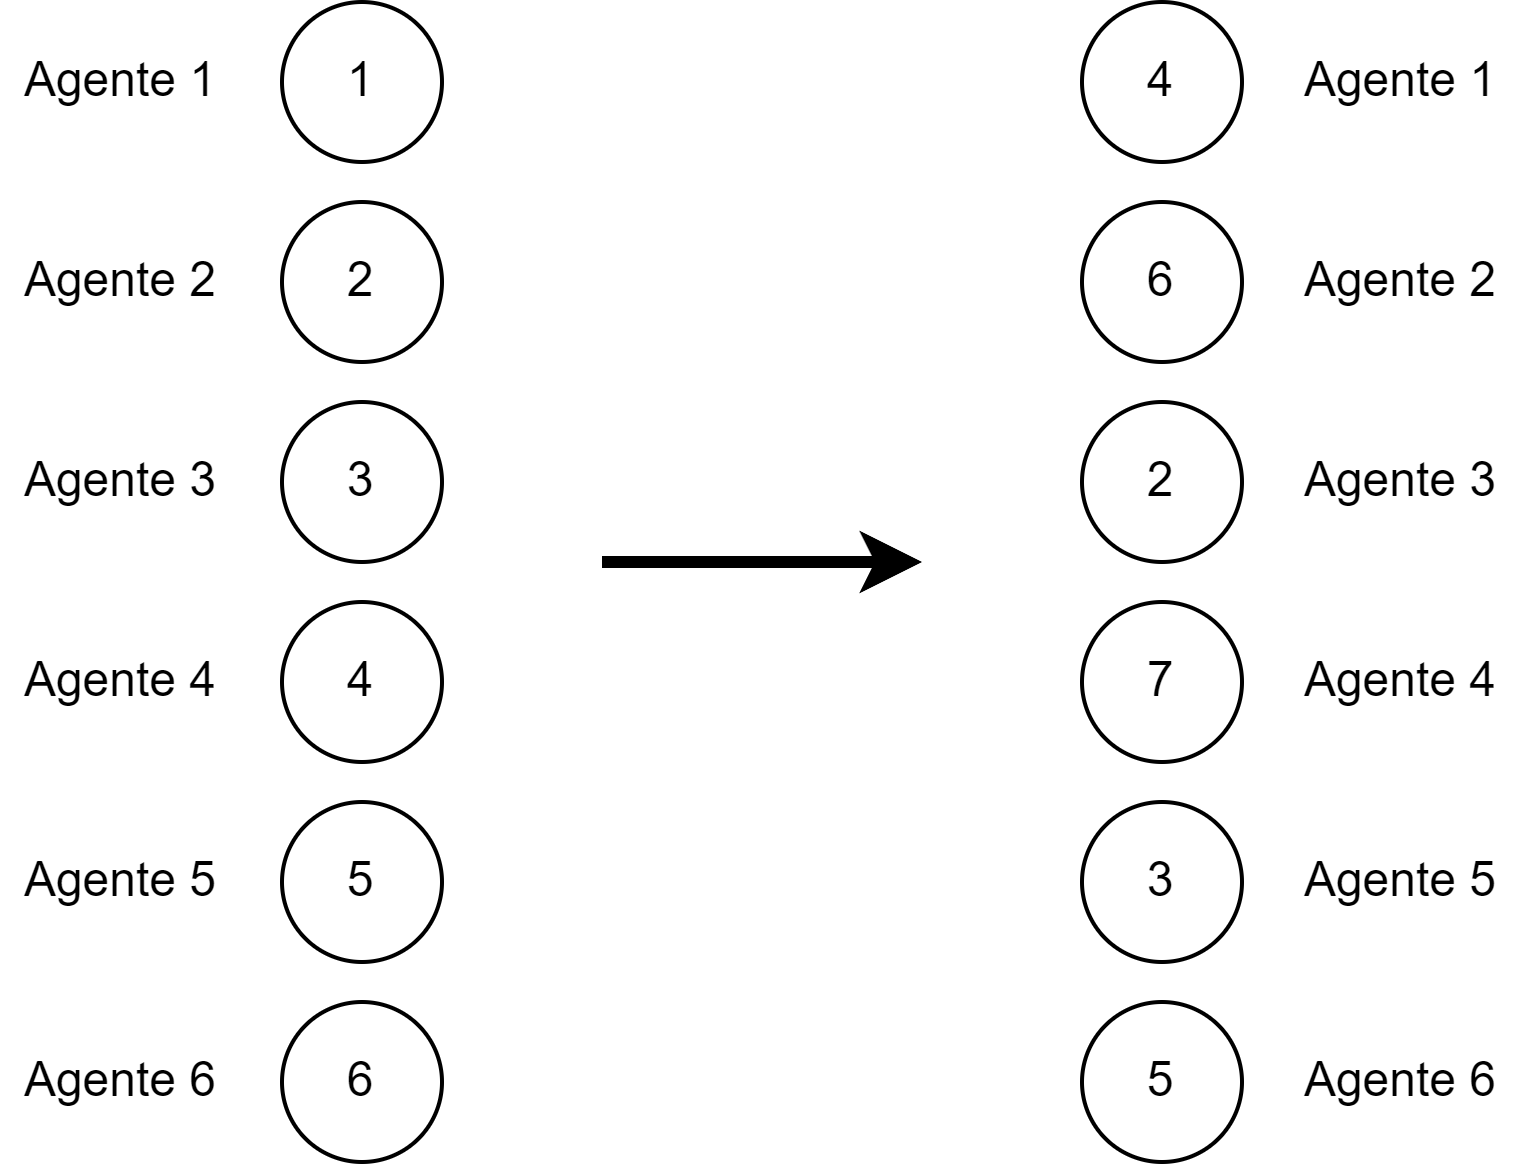
\includegraphics[width=0.6\textwidth]{replicar_fisico_pruebas/seleccion_agentes.png}
	\caption{Selección de marcadores para cada agente. A la izquierda se observa como era la asignación anteriormente y a la derecha como es una selección arbitraria actualmente.}
	\label{fig:seleccion_agentes}
\end{figure}


\subsection{Ajuste de parámetros en el algoritmo}
Luego de las modificaciones anteriores, al ejecutar el algoritmo en físico con tres agentes se encontró que su comportamiento era divergente en la etapa donde se movilizan hacia sus posiciones iniciales. En la Figura \ref{fig:divergencia1} se observa la trayectoria que toman los agentes.

\begin{figure}[H]
	\centering
	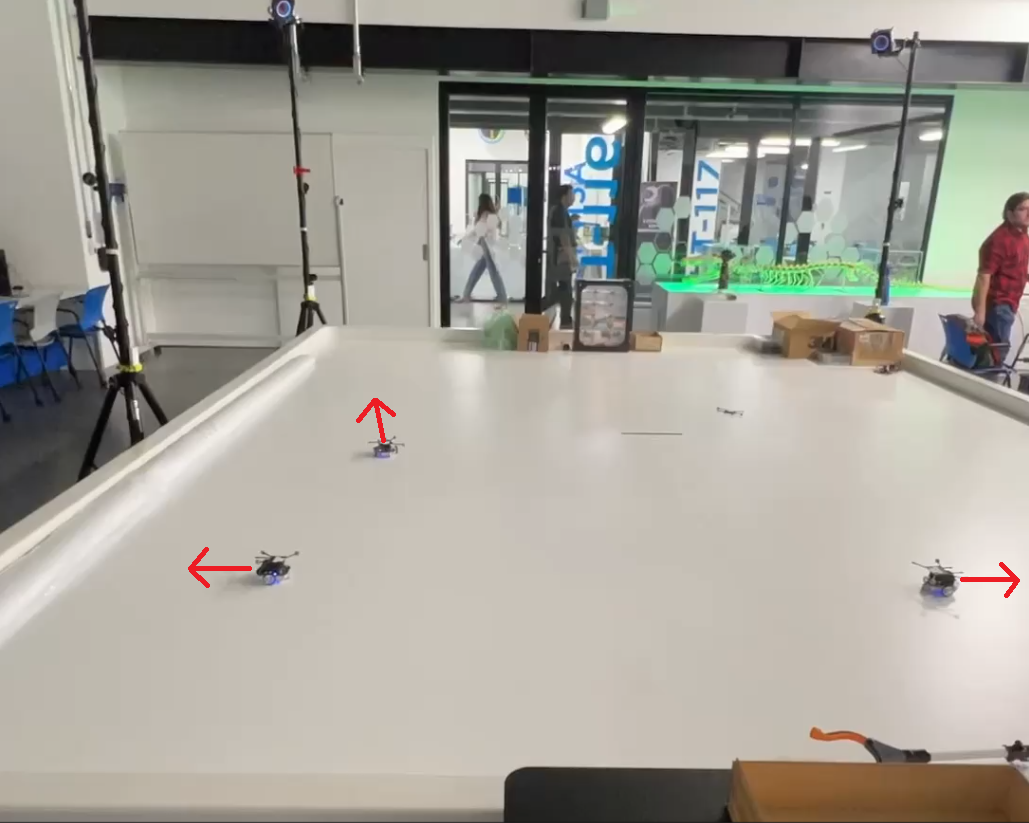
\includegraphics[width=0.45\textwidth]{replicar_fisico_pruebas/divergencia_p1.png}
	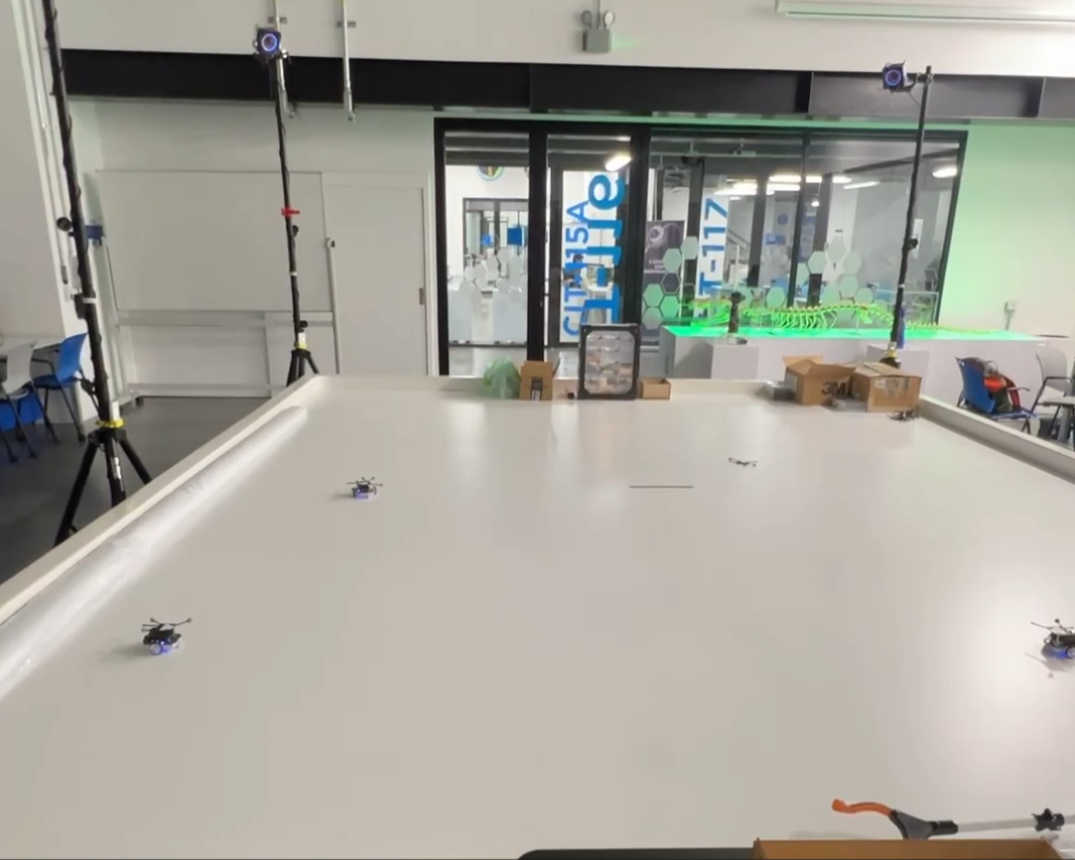
\includegraphics[width=0.45\textwidth]{replicar_fisico_pruebas/divergencia_p2.png}
	\caption{Problema de funcionamiento en físico, agentes divergen hacia posiciones iniciales. }
	\label{fig:divergencia1}
\end{figure}

Para intentar solucionar esto, se invirtió el signo de la constante de proporcionalidad en el control de velocidad aplicado en la etapa 0 del algoritmo. Al realizar el cambio, se encontró que ahora los agentes si se colocan en sus posiciones iniciales, sin embargo, el comportamiento de divergencia se sigue presentando de manera consistente en las demás etapas del algoritmo, tal como se observa en la Figura \ref{fig:divergencia2}, por lo que se optó por revertir el cambio.

\begin{figure}[H]
	\centering
	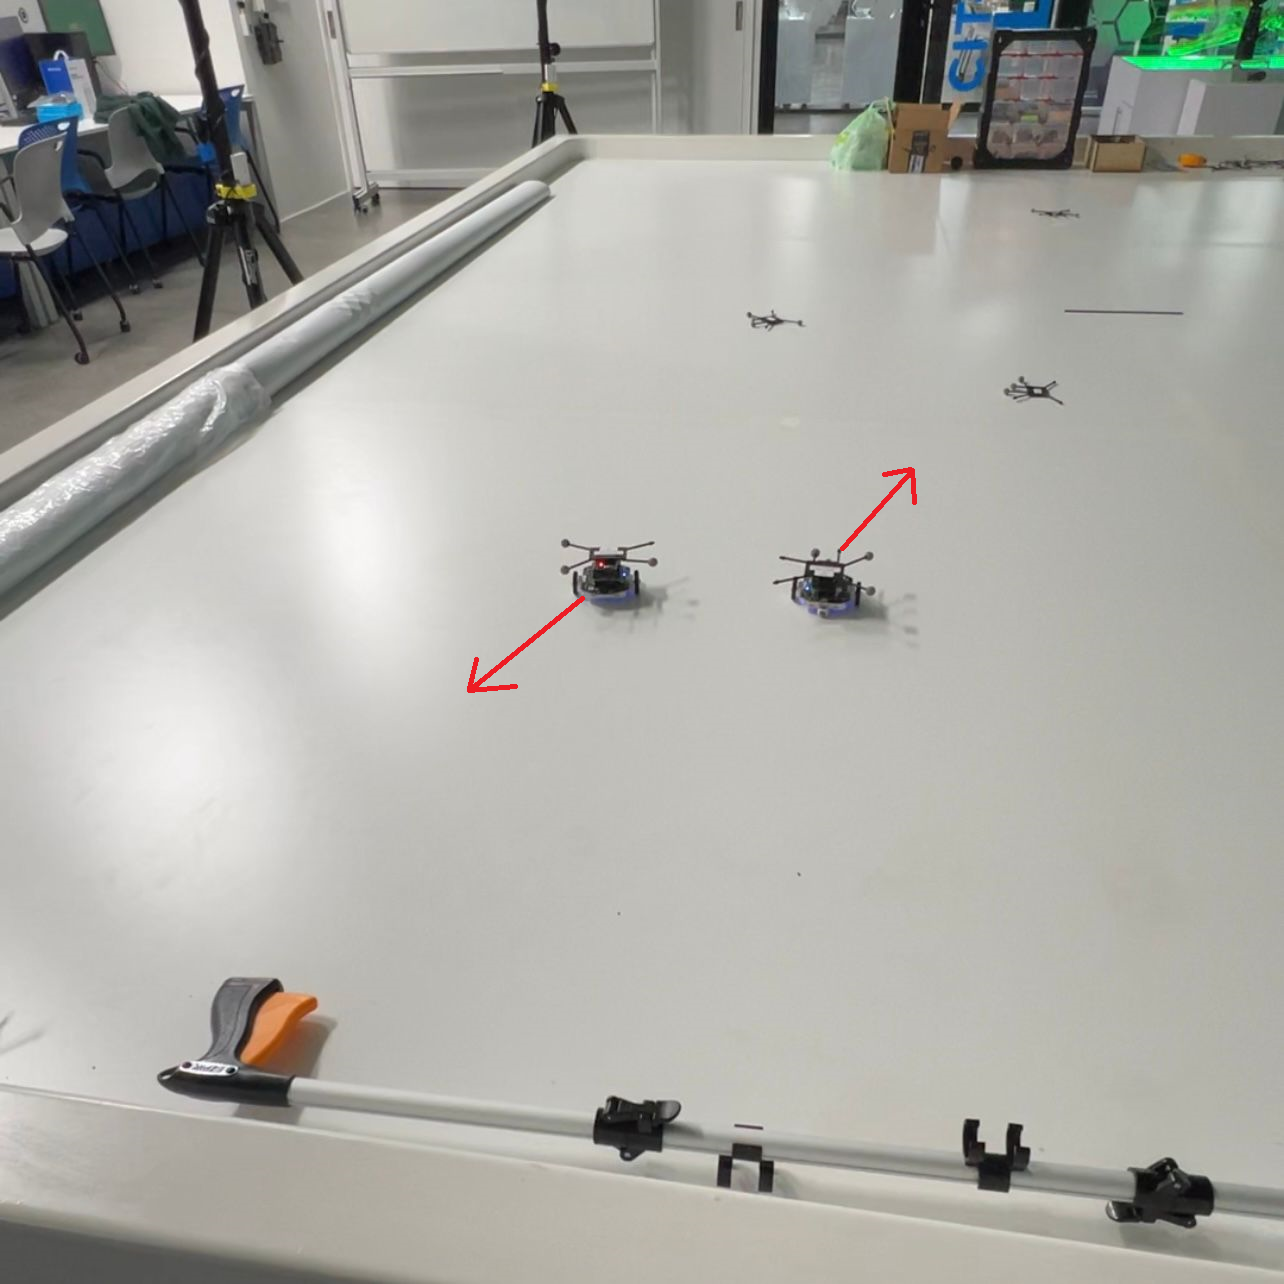
\includegraphics[width=0.45\textwidth]{replicar_fisico_pruebas/divergencia2_p1.png}
	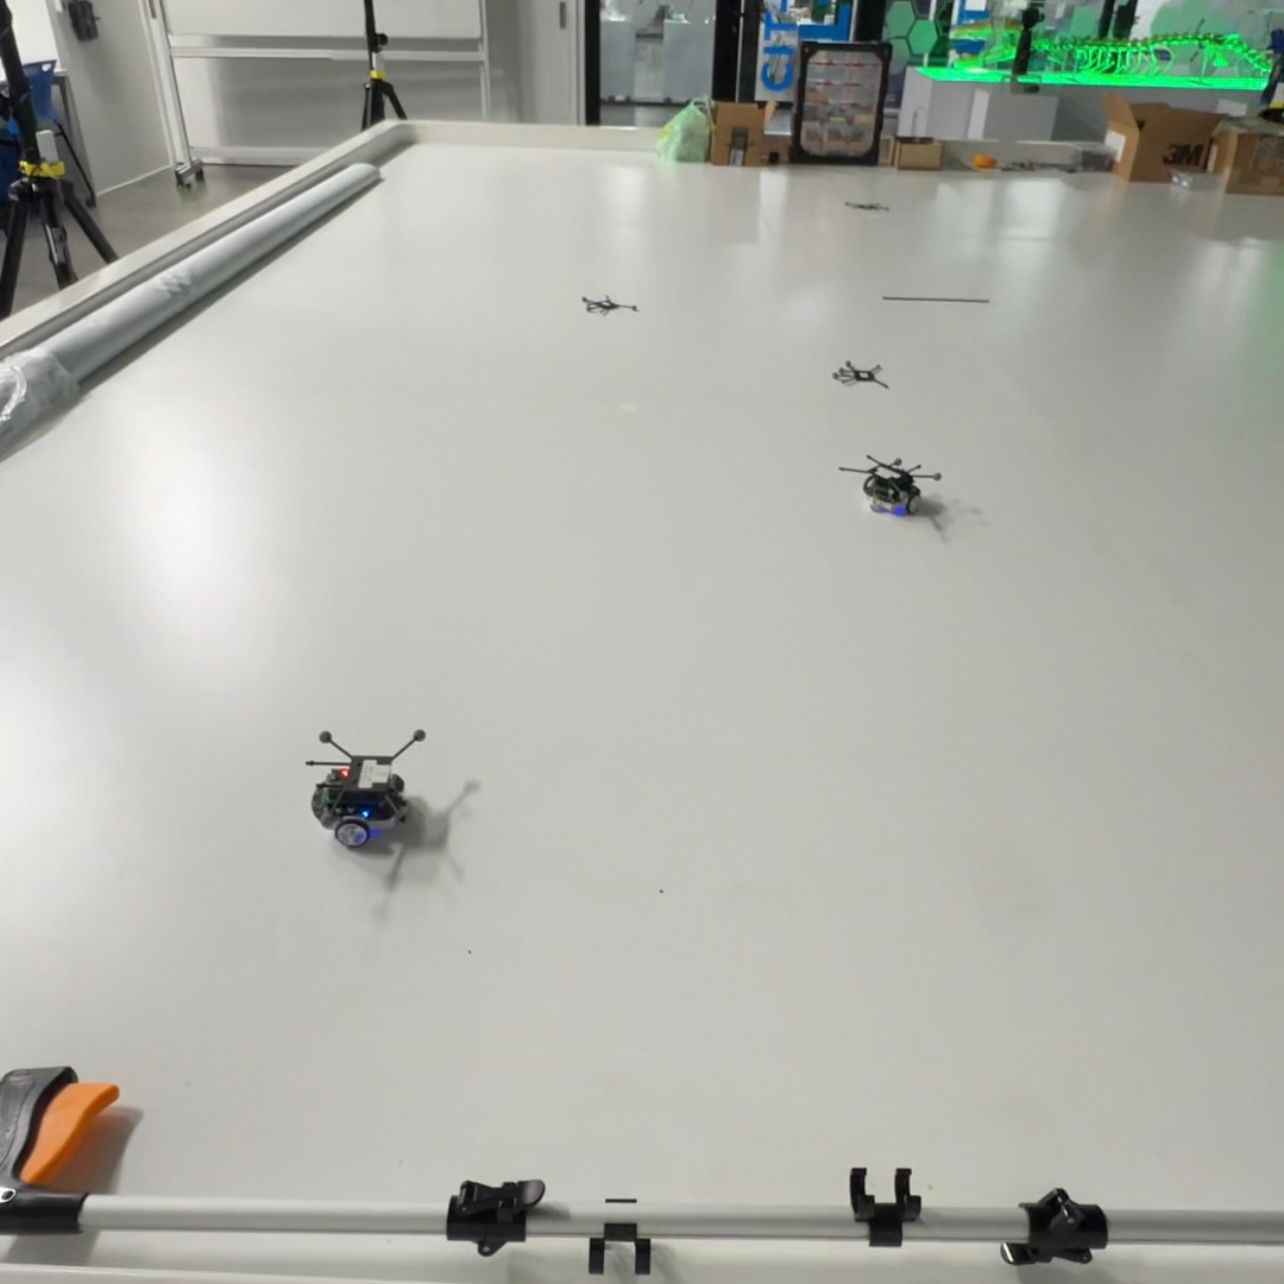
\includegraphics[width=0.45\textwidth]{replicar_fisico_pruebas/divergencia2_p2.png}
	\caption{Problema de funcionamiento en físico, agentes divergen luego de colocarse en sus posiciones iniciales.}
	\label{fig:divergencia2}
\end{figure}

Al analizar el patrón de divergencia, se observó que los agentes se movían en dirección contraria a la esperada. Con esto, se determinó que la causa estaba relacionada con la dirección de movimiento y la rotación de los agentes. En la fase actual, el proceso de calibración de los marcadores se realizó igual que en la fase previa donde los marcadores están alineados con el eje $y$ del Robotat, mientras que los agentes del algoritmo en Webots están alineados con el eje $x$. En la fase previa, esta discrepancia se corregía aplicando un desfase de compensación adicional de $+90^{\circ}$ al ángulo $\theta_z$. Sin embargo, debido a cambios en la infraestructura del Robotat, en esta fase fue necesario invertir dicho desfase a $-90^{\circ}$ para mantener la consistencia en la orientación de los agentes entre lo programado con la simulación y el Robotat. Con esta modificación, se logró replicar correctamente el funcionamiento del algoritmo tanto en el entorno de simulación de Webots como en el Robotat.

\subsection{Configuraciones para el escenario}
Para clasificar las ejecuciones del algoritmo según las condiciones del escenario, se decidió utilizar la misma convención implementada en la fase previa. Esta se enfoca en diferenciar los escenarios según las posiciones de las marcas iniciales para los agentes, los obstáculos y el objetivo.

En el Cuadro \ref{cuadro:configuraciones_escenario} se muestra la codificación utilizada para los experimentos. El orden para identificarlos es el siguiente: (Posición inicial de los agentes)-(Obstáculos)-(Objetivo). A continuación, se presenta el ejemplo de clasificación A-D-B, que significa:

\begin{itemize}
	\item Posicionamiento inicial de los agentes en línea.
	\item Obstáculos móviles.
	\item Objetivo en el centro de la mesa de pruebas.
\end{itemize}

\begin{table}[H]
	\centering
	\resizebox{\textwidth}{!} {
		\begin{tabular}{|l|l|l|l|}
			\hline
			\textbf{Letra de designación} & \textbf{Posición inicial de los agentes} & \textbf{Obstáculos}                                                         & \textbf{Objetivo} \\ \hline
			A                              & Línea                                    & Ninguno                                                                     & Esquina           \\ \hline
			B                              & Círculo                                  & \begin{tabular}[c]{@{}l@{}}1 = Centro\\ 2 = Cerca del objetivo\end{tabular} & Centro            \\ \hline
			C                              & Aleatorio                                & Aleatorio                                                                   & Aleatorio         \\ \hline
			D                              & N/A                                      & Móviles                                                                     & Móvil             \\ \hline
	\end{tabular}}
	\caption{Configuraciones para el escenario.}
	\label{cuadro:configuraciones_escenario}
\end{table}

\subsection{Prueba del algoritmo en físico con escenarios previos}
Una vez solucionados los problemas anteriores, se realizaron las primeras pruebas para replicar algunos de los escenarios físicos realizados en la fase previa y comprobar el funcionamiento correcto del algoritmo.

El código del supervisor ya contaba con un sistema de guardado de información. Este almacena en un archivo .npz todos los datos relevantes al final del experimento. Además, con el archivo ``data\_graphing.py'' se generan las gráficas y trayectorias a partir de que los agentes se hayan colocado en sus posiciones iniciales.

A continuación, se muestran algunos de los datos almacenados más relevantes:

\begin{itemize}
	\item Historial durante todo el experimento de:
	\begin{itemize}
		\item Posiciones y orientaciones de los agentes
		\item Posiciones de los obstáculos
		\item Posición del objetivo
		\item Velocidades de los agentes
	\end{itemize}
	\item Datos y configuraciones de:
	\begin{itemize}
		\item Ciclos del experimento
		\item Ciclo en que se logra el objetivo
		\item Ciclo en que inicia la etapa 1 del algoritmo
		\item Cantidad de agentes y sus números de marcadores asignados
		\item Cantidad de obstáculos y sus números de marcadores asignados
		\item Marcas de posiciones iniciales de los agentes
		\item Paso de tiempo del programa
	\end{itemize}
\end{itemize}

\subsubsection{Primer escenario}
Para el primer escenario, se utilizó la configuración AAA con 2 agentes. En la Figura \ref{fig:test_fisico1} se muestra el escenario en la mesa de pruebas con los agentes antes de colocarse en sus posiciones iniciales y en la Figura \ref{fig:traj_test_2A_AAA_f_1} las trayectorias de los agentes luego de colocarse en sus posiciones iniciales.

\begin{figure}[H]
	\centering
	\includegraphics[width=0.45\textwidth]{replicar_fisico_escenarios/test_f1v2.png}
	\caption{Mesa de pruebas con 2 agentes en el escenario AAA, corrida 1, en físico.}
	\label{fig:test_fisico1}
\end{figure}
\begin{figure}[H]
	\centering
	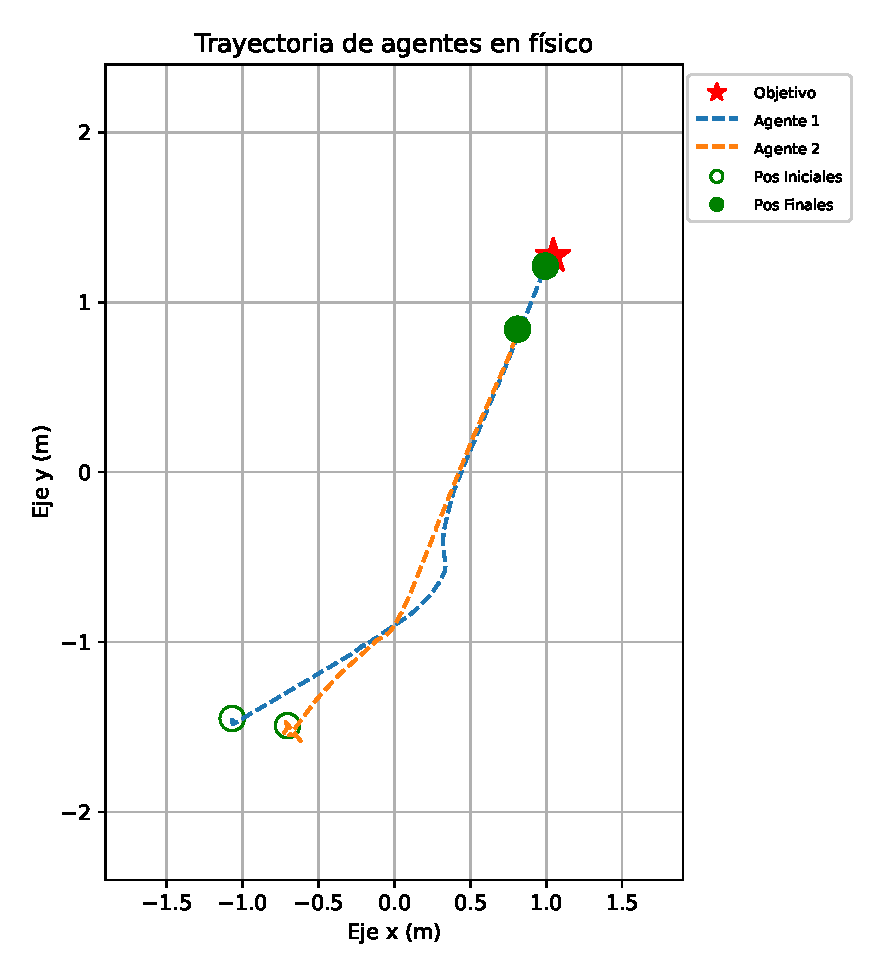
\includegraphics[width=0.45\textwidth]{replicar_fisico_escenarios/traj_test_2A_AAA_f_1.eps}
	\caption{Trayectoria de los 2 agentes en el escenario AAA, corrida 1, en físico.}
	\label{fig:traj_test_2A_AAA_f_1}
\end{figure}

\subsubsection{Segundo escenario}
Para el segundo escenario, se utilizó la configuración AAA con 6 agentes. En la Figura \ref{fig:test_fisico2} se muestra el escenario en la mesa de pruebas con los agentes antes de colocarse en sus posiciones iniciales y en la Figura \ref{fig:traj_test_6A_AAA_f_1} las trayectorias de los agentes luego de colocarse en sus posiciones iniciales. 

Para este escenario, se observó que las trayectorias no son igual de sencillas y directas que con el primer escenario. Esto es ya que, al tener más agentes, estos ajustan sus trayectorias para mantener su posición en la formación evitando colisionar entre sí, al mismo tiempo que mantienen una distancia de seguridad ante colisiones.

\begin{figure}[H]
	\centering
	\includegraphics[width=0.45\textwidth]{replicar_fisico_escenarios/test_f2v2.png}
	\caption{Mesa de pruebas con 6 agentes en el escenario AAA, corrida 1, en físico.}
	\label{fig:test_fisico2}
\end{figure}
\begin{figure}[H]
	\centering
	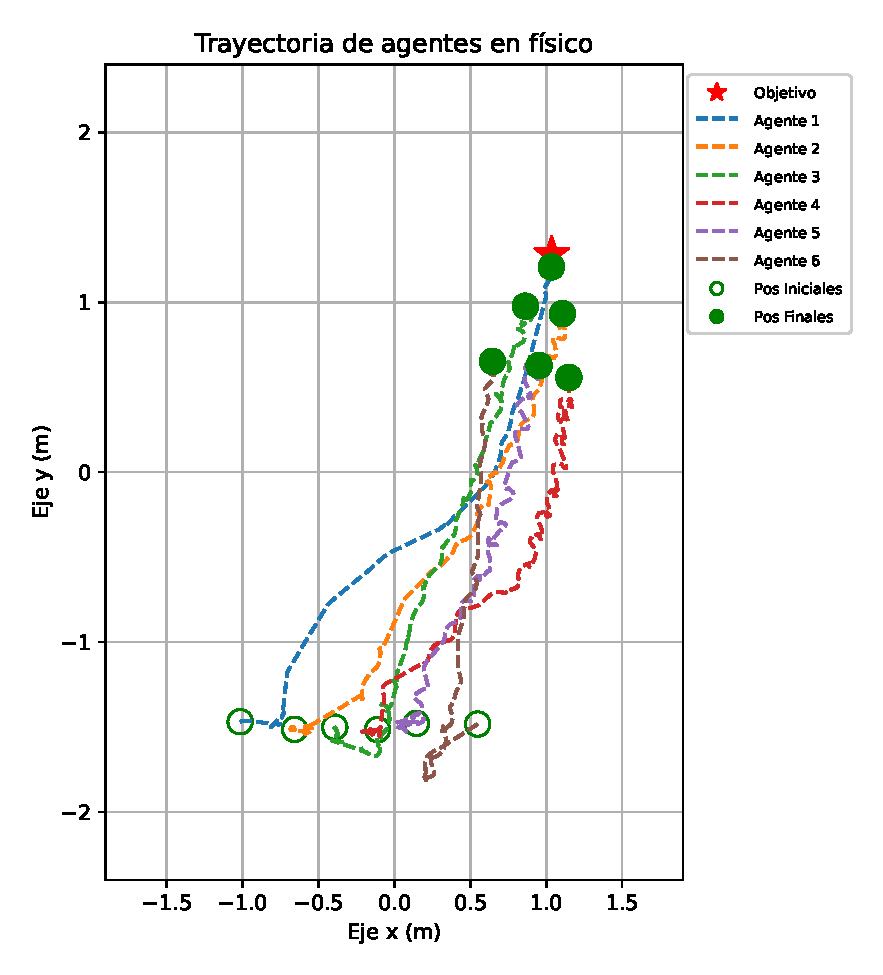
\includegraphics[width=0.45\textwidth]{replicar_fisico_escenarios/traj_test_6A_AAA_f_1.eps}
	\caption{Trayectoria de los 6 agentes en el escenario AAA, corrida 1, en físico.}
	\label{fig:traj_test_6A_AAA_f_1}
\end{figure}

\subsubsection{Tercer escenario}
Para el tercer escenario, se utilizó la configuración ACA con 6 agentes. En la Figura \ref{fig:test_fisico3} se muestra el escenario en la mesa de pruebas con los agentes antes de colocarse en sus posiciones iniciales y en la Figura \ref{fig:traj_test_6A_ACA_f_1} las trayectorias de los agentes luego de colocarse en sus posiciones iniciales.

Este escenario fue configurado como el segundo escenario con la adición de tres obstáculos. En las trayectorias de los agentes, se observa que estos lograron mantener su formación y evitaron los obstáculos al trasladarse entre ellos. Además, se observa con la complejidad de las trayectorias, que los agentes se estuvieron movilizando para evitar colisionar entre sí y mantener su posición en la formación.

\begin{figure}[H]
	\centering
	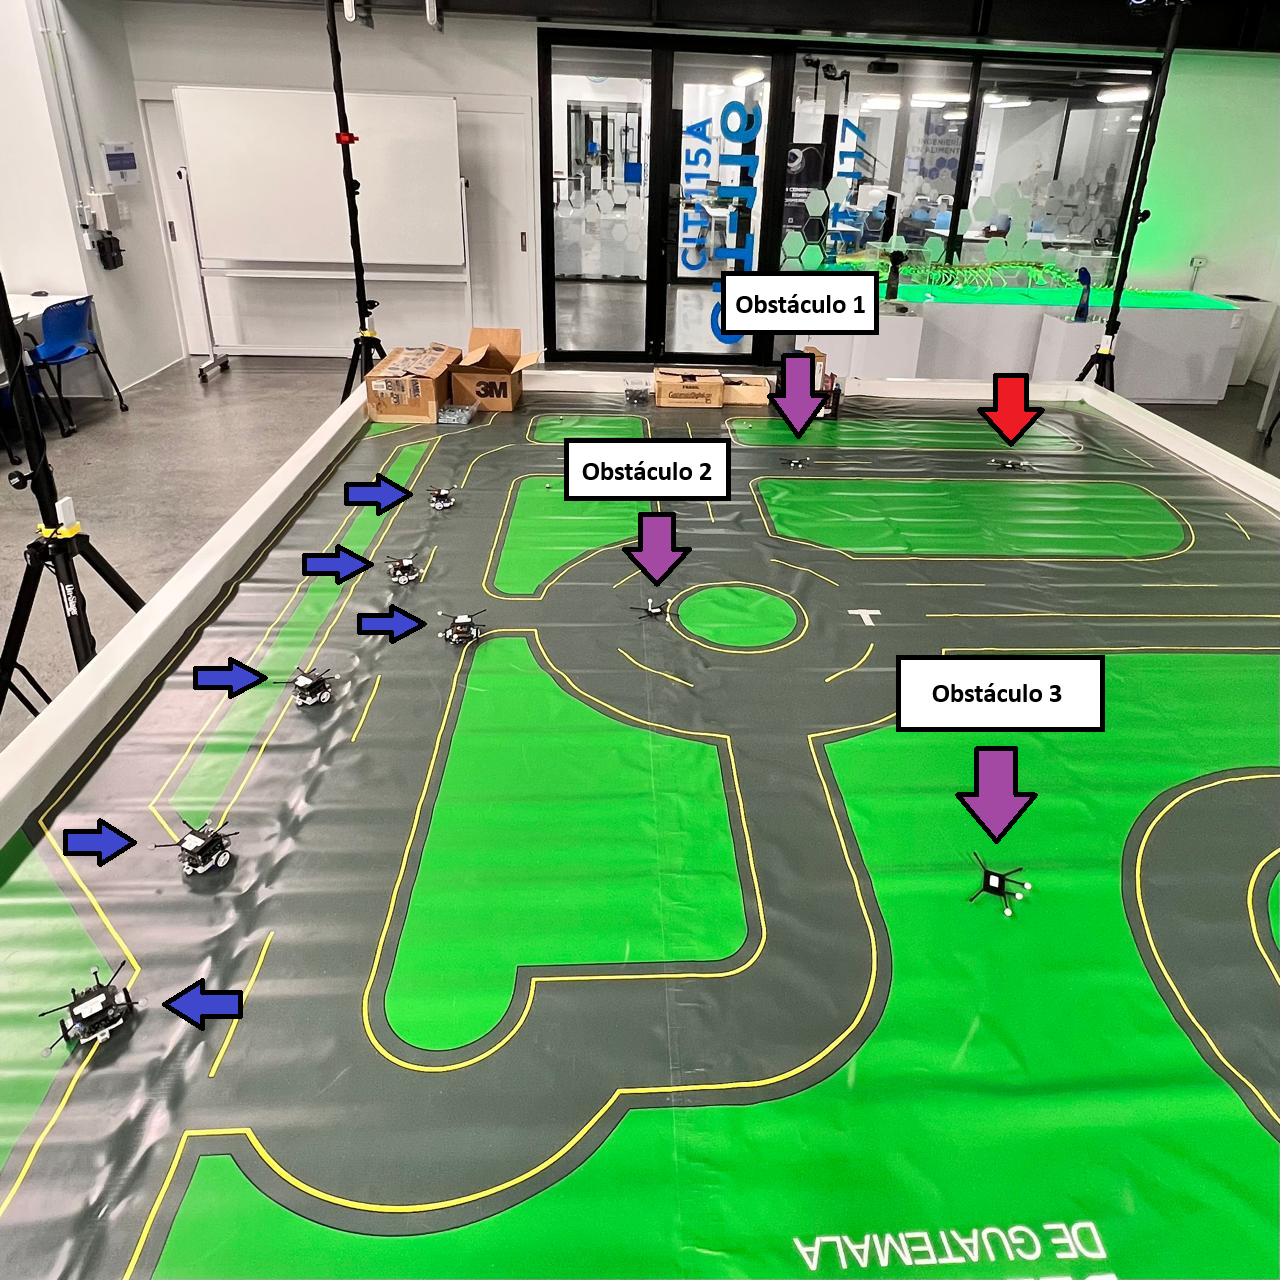
\includegraphics[width=0.45\textwidth]{replicar_fisico_escenarios/test_f3v2.png}
	\caption{Mesa de pruebas con 6 agentes en el escenario ACA, corrida 1, en físico.}
	\label{fig:test_fisico3}
\end{figure}
\begin{figure}[H]
	\centering
	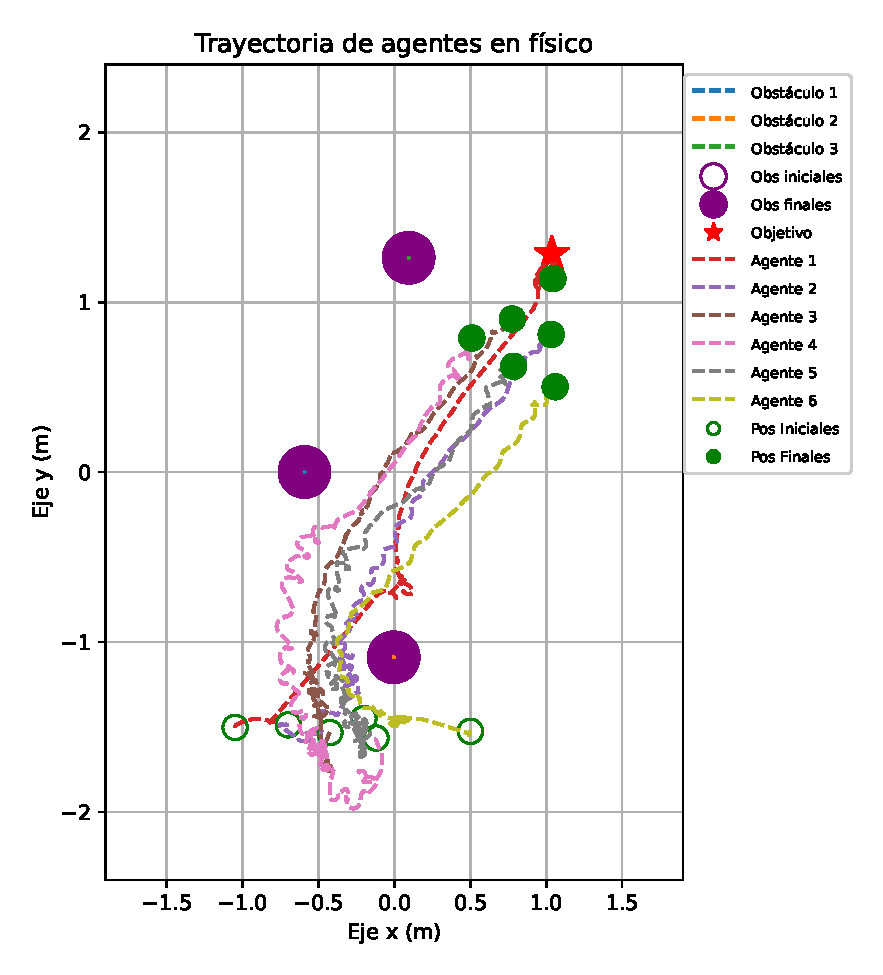
\includegraphics[width=0.45\textwidth]{replicar_fisico_escenarios/traj_test_6A_ACA_f_1.eps}
	\caption{Trayectoria de los 6 agentes en el escenario ACA, corrida 1, en físico.}
	\label{fig:traj_test_6A_ACA_f_1}
\end{figure}

\subsubsection{Cuarto escenario}
Para el cuarto escenario, se utilizó la configuración ACC con 3 agentes. En la Figura \ref{fig:test_fisico4} se muestra el escenario en la mesa de pruebas con los agentes antes de colocarse en sus posiciones iniciales y en la Figura \ref{fig:traj_test_3A_ACC_f_1} las trayectorias de los agentes luego de colocarse en sus posiciones iniciales.

Para este escenario también se adicionó tres obstáculos. En las trayectorias, se observa que los agentes lograron evadirlos y pasar entre ellos para llegar al objetivo, además, al tener menos agentes en la formación, las trayectorias fueron más sencillas ya que se tenía menos agentes con los que podrían colisionar entre sí.

\begin{figure}[H]
	\centering
	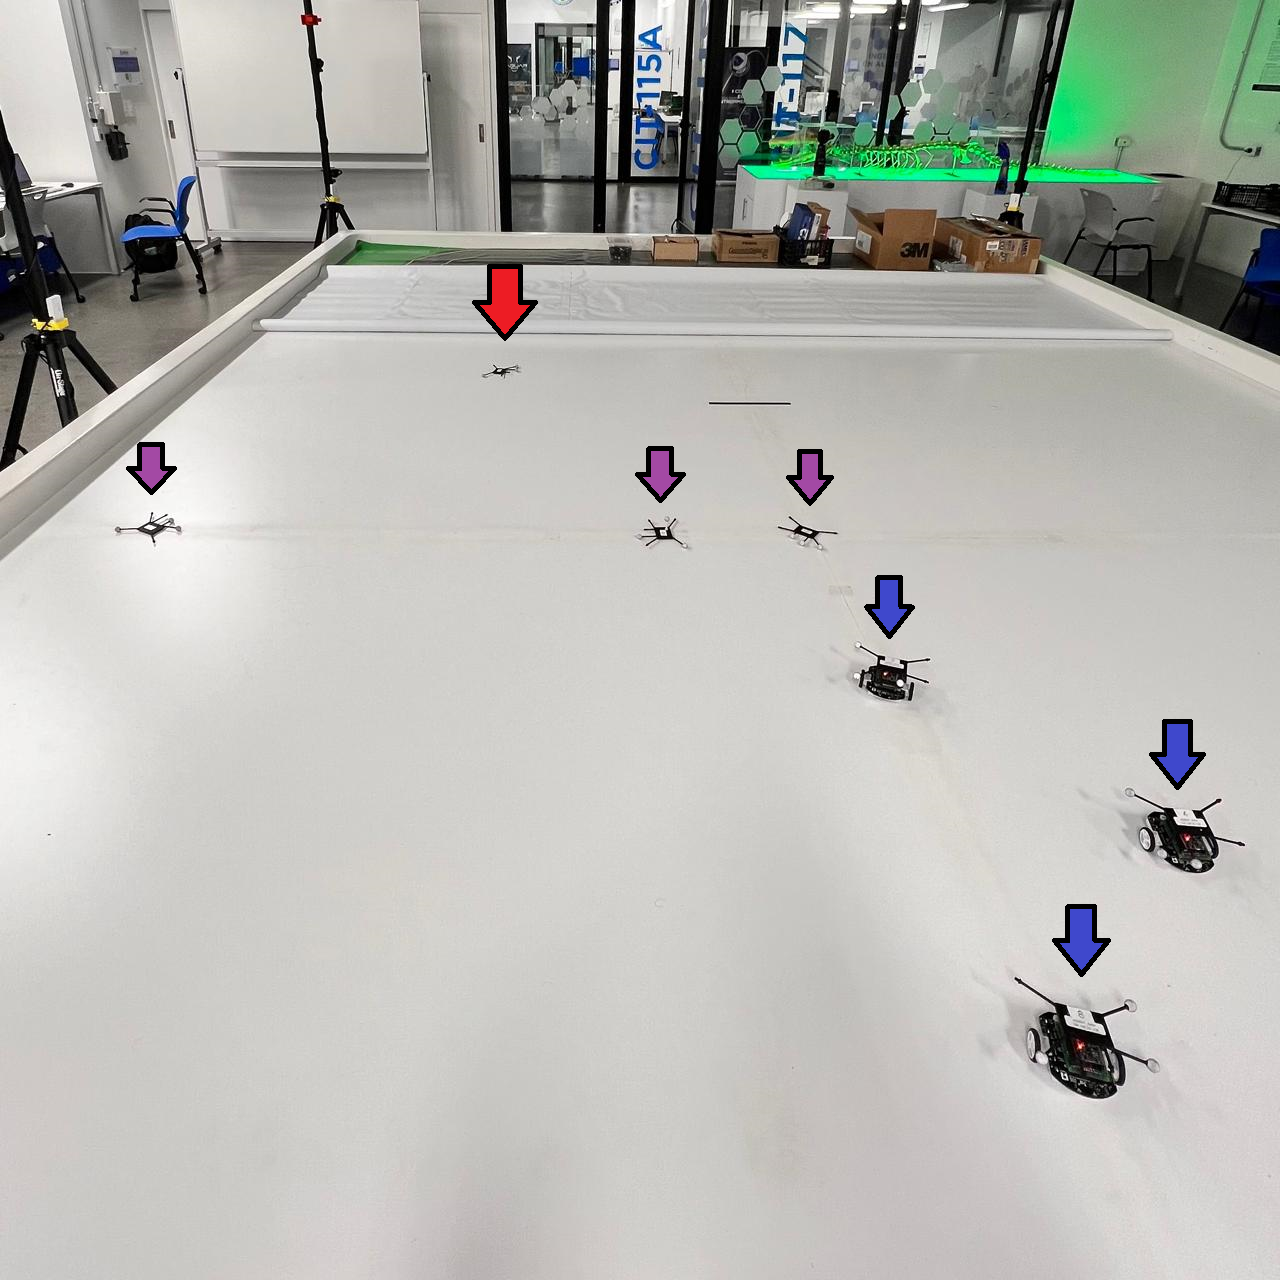
\includegraphics[width=0.45\textwidth]{replicar_fisico_escenarios/test_f4v2.png}
	\caption{Mesa de pruebas con 3 agentes en el escenario ACC, corrida 1, en físico.}
	\label{fig:test_fisico4}
\end{figure}
\begin{figure}[H]
	\centering
	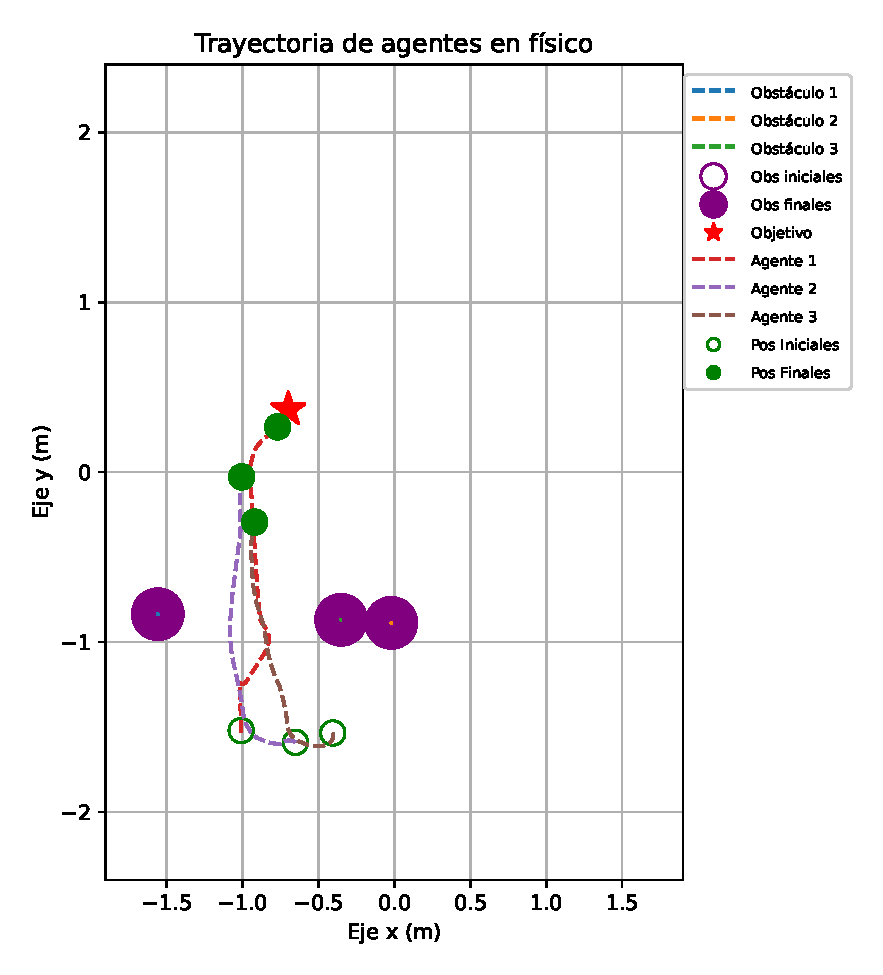
\includegraphics[width=0.45\textwidth]{replicar_fisico_escenarios/traj_test_3A_ACC_f_1.eps}
	\caption{Trayectoria de los 3 agentes en el escenario ACC, corrida 1, en físico.}
	\label{fig:traj_test_3A_ACC_f_1}
\end{figure}

\subsubsection{Quinto escenario}
Para el quinto escenario, se utilizó la configuración ACA con 3 agentes. En la Figura \ref{fig:test_fisico5} se muestra el escenario en la mesa de pruebas con los agentes antes de colocarse en sus posiciones iniciales y en la Figura \ref{fig:traj_test_3A_ACA_f_1} las trayectorias de los agentes luego de colocarse en sus posiciones iniciales.

Para este escenario se agregaron tres obstáculos de manera similar al cuarto escenario. En las trayectorias, se observa que los agentes lograron evadirlos y pasar entre ellos para llegar al objetivo, además, al tener pocos agentes en la formación, las trayectorias fueron más sencillas ya que se tenía menos agentes con los que podrían colisionar entre sí.

\begin{figure}[H]
	\centering
	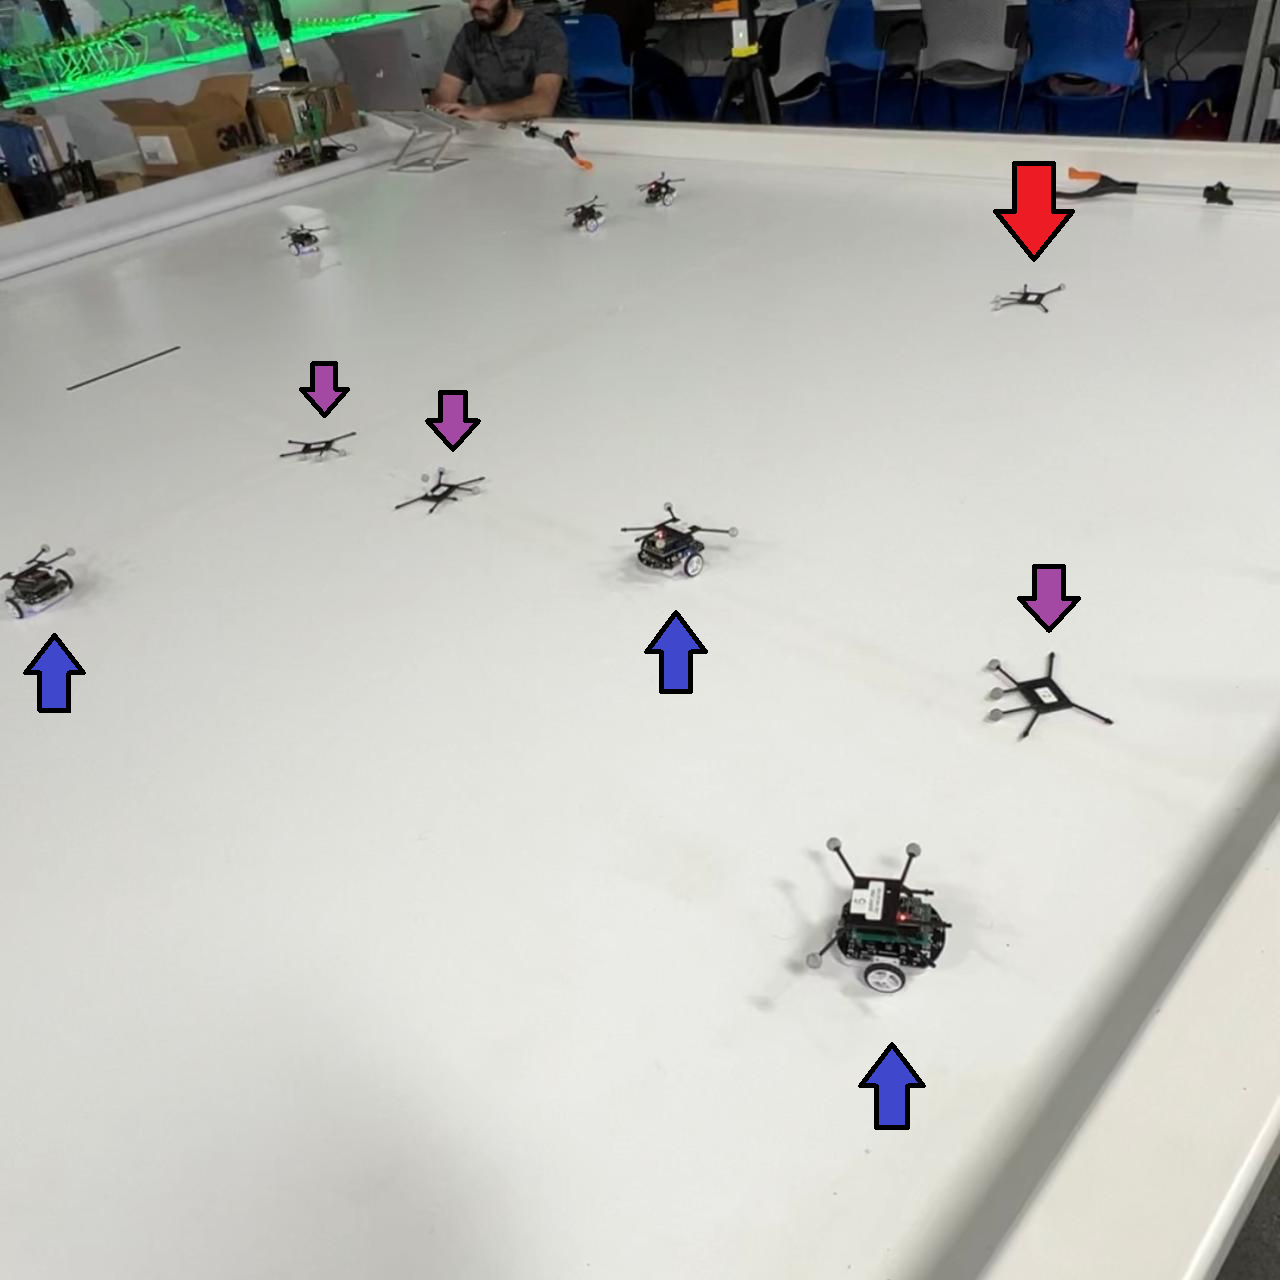
\includegraphics[width=0.45\textwidth]{replicar_fisico_escenarios/test_f5v2.png}
	\caption{Mesa de pruebas con 3 agentes en el escenario ACA, corrida 1, en físico.}
	\label{fig:test_fisico5}
\end{figure}
\begin{figure}[H]
	\centering
	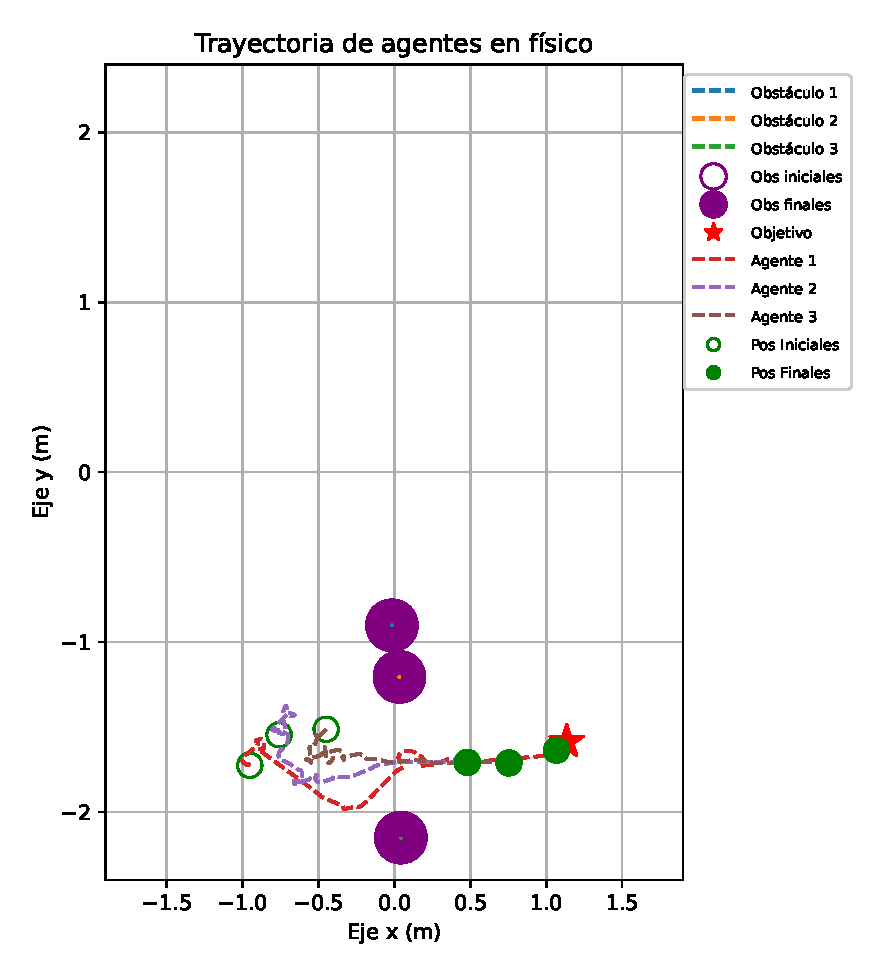
\includegraphics[width=0.45\textwidth]{replicar_fisico_escenarios/traj_test_3A_ACA_f_1.eps}
	\caption{Trayectoria de los 3 agentes en el escenario ACA, corrida 1, en físico.}
	\label{fig:traj_test_3A_ACA_f_1}
\end{figure}

\chapter{Prueba de la naturaleza dinámica del algoritmo con obstáculos móviles}\label{cap:naturaleta_dinamica}
En este capítulo, se explica y se pone a prueba la naturaleza dinámica del algoritmo de sincronización y control de formaciones. 

\section{Naturaleza dinámica del algoritmo}
Como se mencionó anteriormente, se cuenta con el archivo ``data\_graphing.py'' para generar las gráficas y trayectorias del experimento. Sin embargo, este no mostraba el recorrido de los obstáculos en movimiento, por lo que se agregó esta función a manera de visualizar la posición inicial, y final, así como las trayectorias de los obstáculos.

A continuación, se presentan los escenarios en los que se puso a prueba el algoritmo con obstáculos móviles en simulaciones y en físico. En todos los casos, se observa que los agentes lograron reposicionarse y cambiar su trayectoria al moverse los obstáculos, manteniendo su formación mientras siguen el objetivo. Esto es posible gracias a la naturaleza dinámica del algoritmo, que se debe a la manera en que se planteó originalmente la ecuación de consenso y el cálculo del peso para determinar las velocidades de los agentes. Además, el algoritmo está constantemente evaluando la posición actual de cada agente y la compara con la posición actual de los obstáculos. Con esto, se ajusta de forma dinámica el peso $w$ y se re calcula la ecuación de consenso para evitar posibles colisiones.

\newpage
\section{Simulaciones utilizando obstáculos móviles}
Para las simulaciones mostradas en las Figuras \ref{fig:traj_testSim_6A_ADA_v_1}, \ref{fig:traj_testSim_6A_ADA_v_2} y \ref{fig:traj_testSim_6A_ADA_v_3} se optó por utilizar una configuración ADA con 6 agentes y se movilizó los obstáculos a manera de que estos interfirieran con la trayectoria de la formación durante el seguimiento al objetivo. Cabe mencionar que la movilización de los obstáculos se hizo de manera aleatoria y sin ningún patrón en específico. 

\subsection{Primer escenario}
\begin{figure}[H]
	\centering
	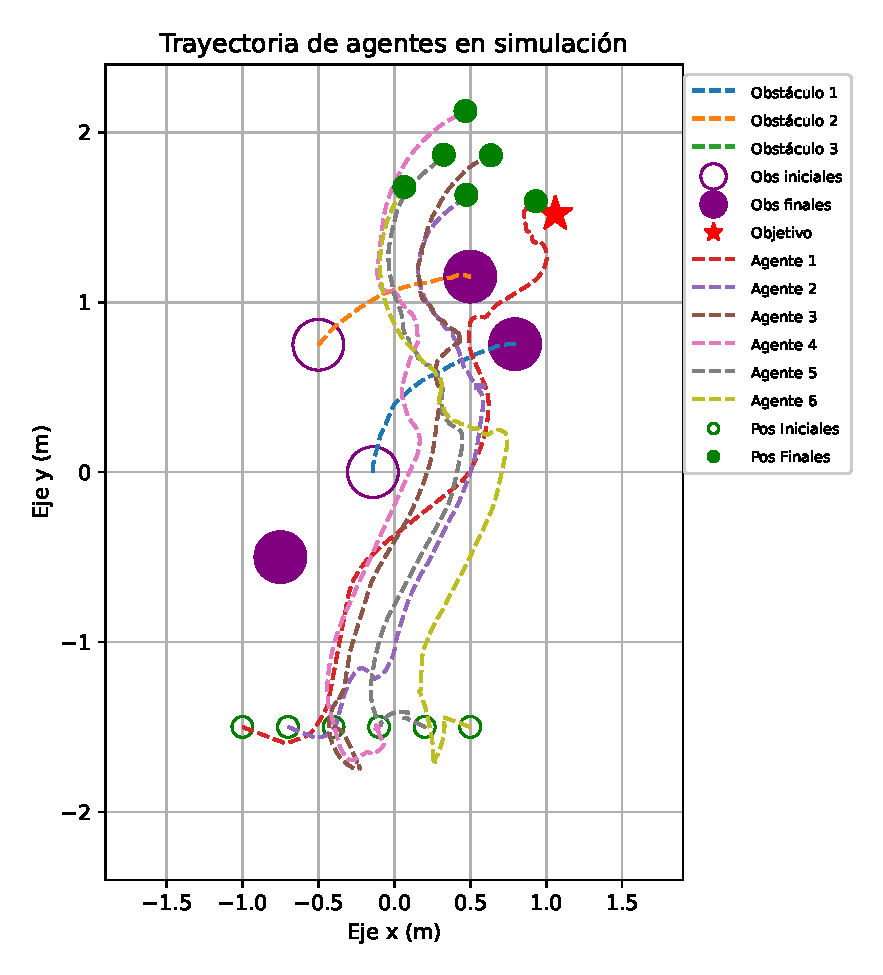
\includegraphics[width=\textwidth]{test_sim_ObsM/traj_testSim_6A_ADA_v_1.eps}
	\caption{Trayectoria de los 6 agentes en el escenario ADA, corrida 1, en simulación.}
	\label{fig:traj_testSim_6A_ADA_v_1}
\end{figure}

\subsection{Segundo escenario}
\begin{figure}[H]
	\centering
	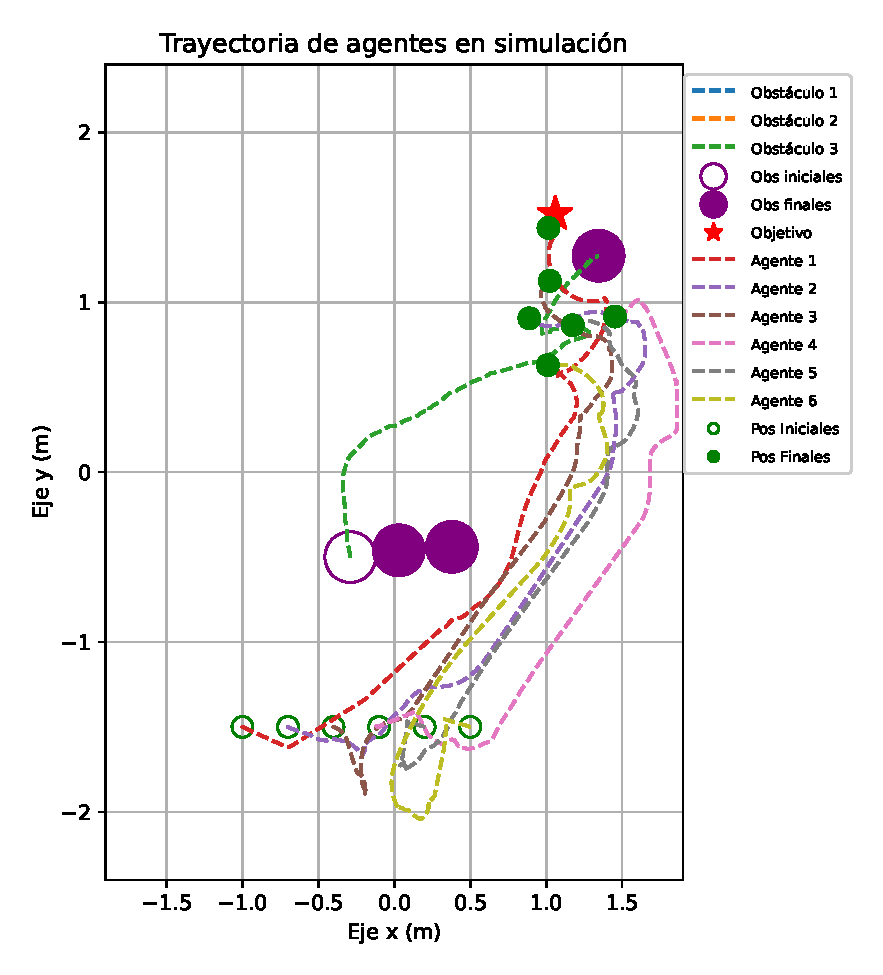
\includegraphics[width=\textwidth]{test_sim_ObsM/traj_testSim_6A_ADA_v_2.eps}
	\caption{Trayectoria de los 6 agentes en el escenario ADA, corrida 2, en simulación.}
	\label{fig:traj_testSim_6A_ADA_v_2}
\end{figure}

\subsection{Tercer escenario}
\begin{figure}[H]
	\centering
	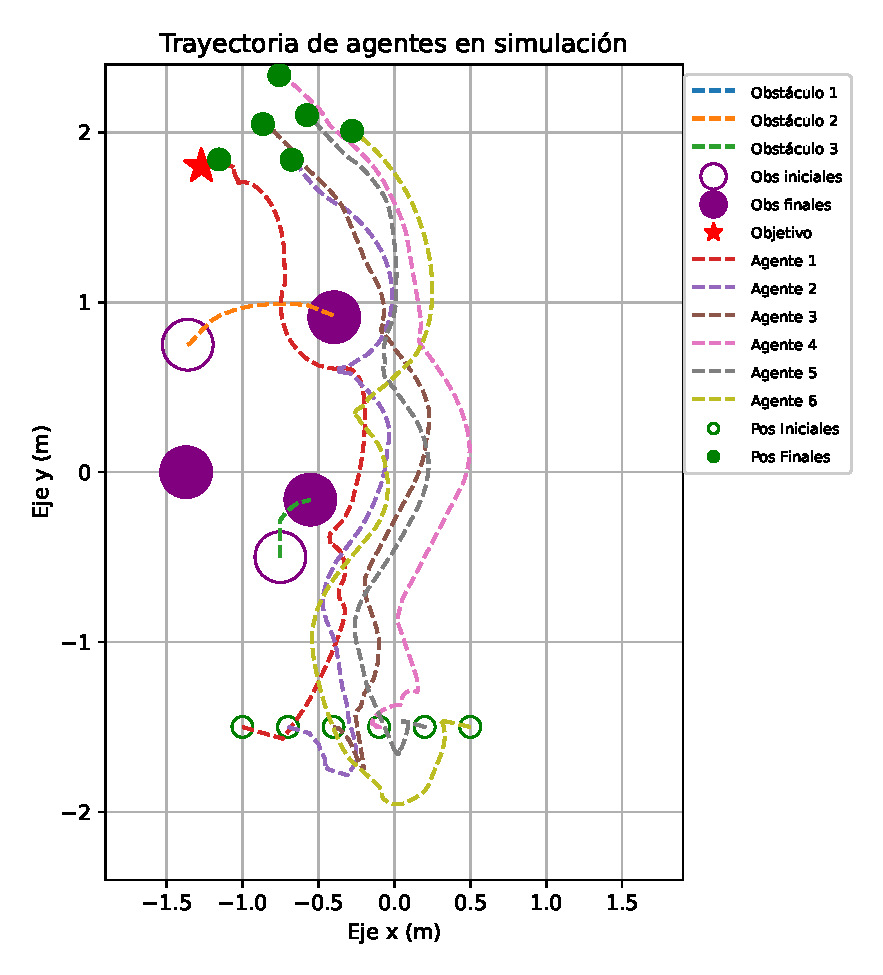
\includegraphics[width=\textwidth]{test_sim_ObsM/traj_testSim_6A_ADA_v_3.eps}
	\caption{Trayectoria de los 6 agentes en el escenario ADA, corrida 3, en simulación.}
	\label{fig:traj_testSim_6A_ADA_v_3}
\end{figure}


\section{Escenarios físicos utilizando obstáculos móviles}
A diferencia que con los escenarios en simulaciones, para las pruebas en físico se movilizó los obstáculos a manera de que estos interfirieran o liberaran una trayectoria de la formación durante el seguimiento al objetivo.

\subsection{Primer escenario}
Para este escenario, se movilizaron los obstáculos para que estos dejaran libre la trayectoria de los agentes hacia el objetivo en lugar de interferir en esta. Como se observa en la Figura \ref{fig:traj_test_3A_ADB_f_1}, el agente 1 con la trayectoria roja, pasa sobre la posición donde se encontraba el obstáculo inicialmente. Además, evita colisionar con los obstáculos colocados en sus posiciones finales. 

\begin{figure}[H]
	\centering
	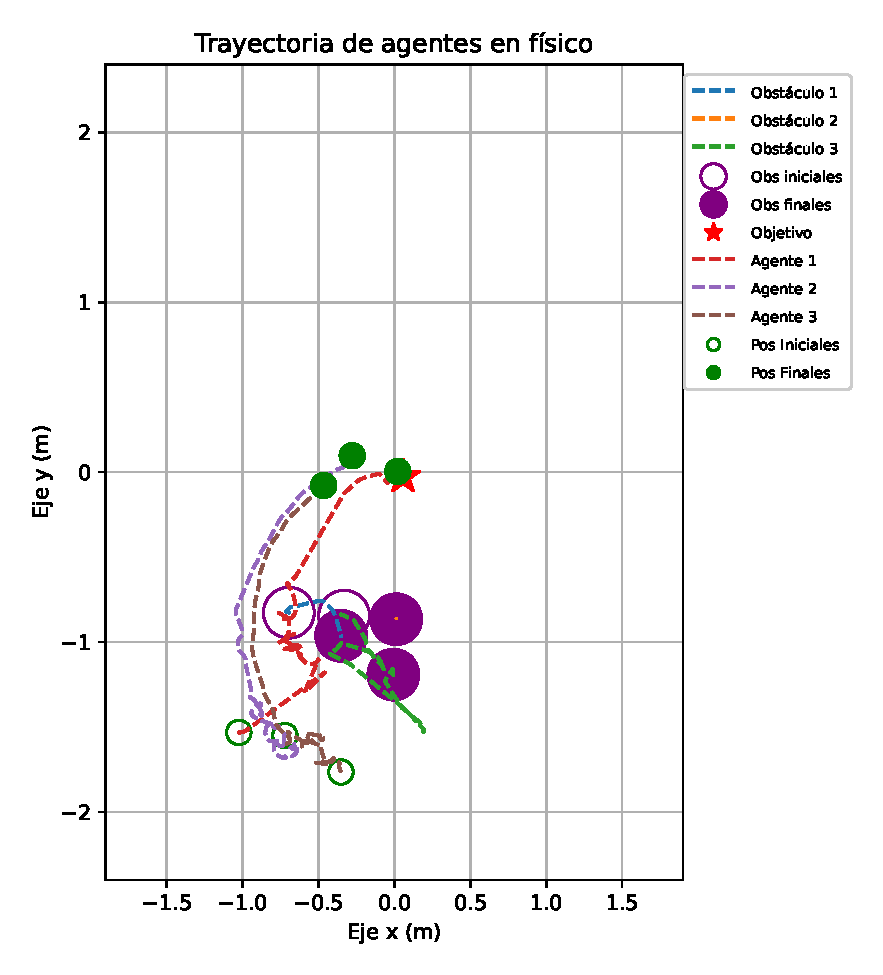
\includegraphics[width=\textwidth]{test_fisico_ObsM/traj_test_3A_ADB_f_1.eps}
	\caption{Trayectoria de los 3 agentes en el escenario ADB, corrida 1, en físico.}
	\label{fig:traj_test_3A_ADB_f_1}
\end{figure}

\subsection{Segundo escenario}
Para este escenario, se planteó el recorrido a manera que los agentes tuvieran que pasar en medio de los obstáculos. Como se observa en la Figura \ref{fig:traj_test_3A_ADC_f_1}, con la trayectoria en verde, el obstáculo se movilizó a lo largo del espacio libre para que este bloqueara el camino hacia el objetivo. Luego se volvió a colocar cercano a su posición inicial. Además, se observa cómo los agentes lograron evitar la colisión y seguir su trayecto una vez que el camino se liberara.
\begin{figure}[H]
	\centering
	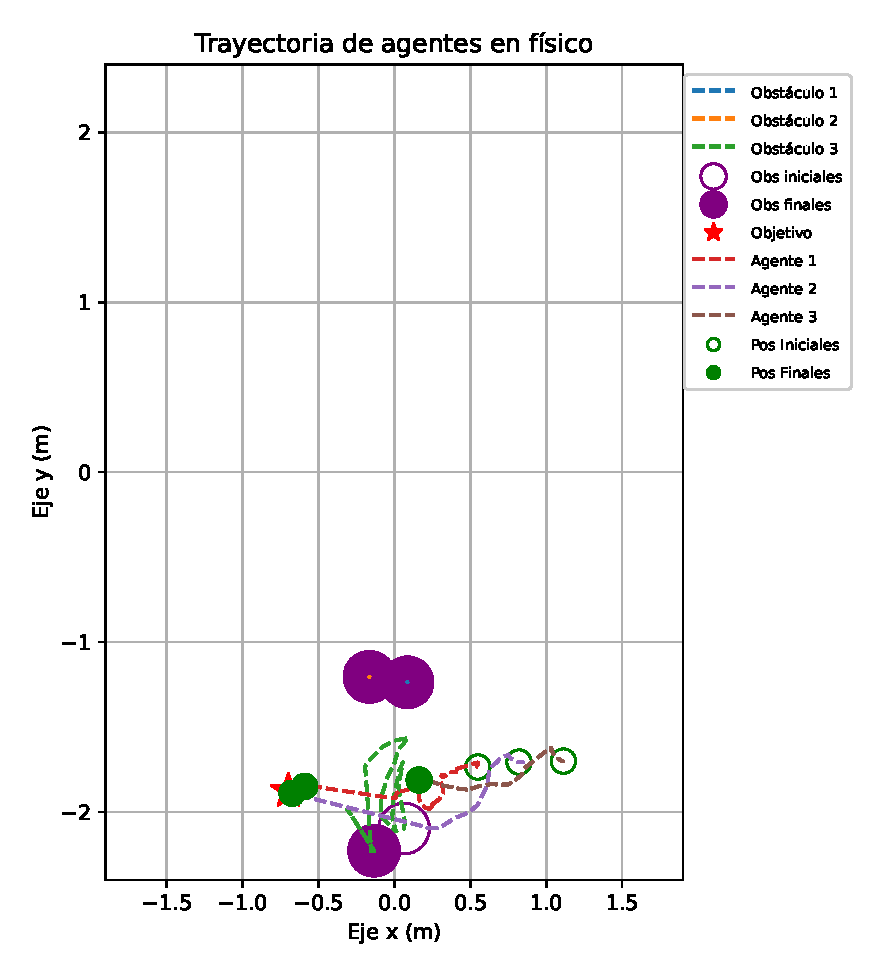
\includegraphics[width=\textwidth]{test_fisico_ObsM/traj_test_3A_ADC_f_1.eps}
	\caption{Trayectoria de los 3 agentes en el escenario ADC, corrida 1, en físico.}
	\label{fig:traj_test_3A_ADC_f_1}
\end{figure}

\subsection{Tercer escenario}
Para este caso, se realizó lo mismo que en el segundo escenario. Como se observa en la Figura \ref{fig:traj_test_3A_ADC_f_3}, con la trayectoria en verde, el obstáculo se movilizó a lo largo del espacio libre a manera que este bloqueara el camino hacia el objetivo. Luego se volvió a colocar cercano a su posición inicial, donde se observa cómo los agentes lograron evitar la colisión y seguir su trayecto una vez que el camino se liberara.

\begin{figure}[H]
	\centering
	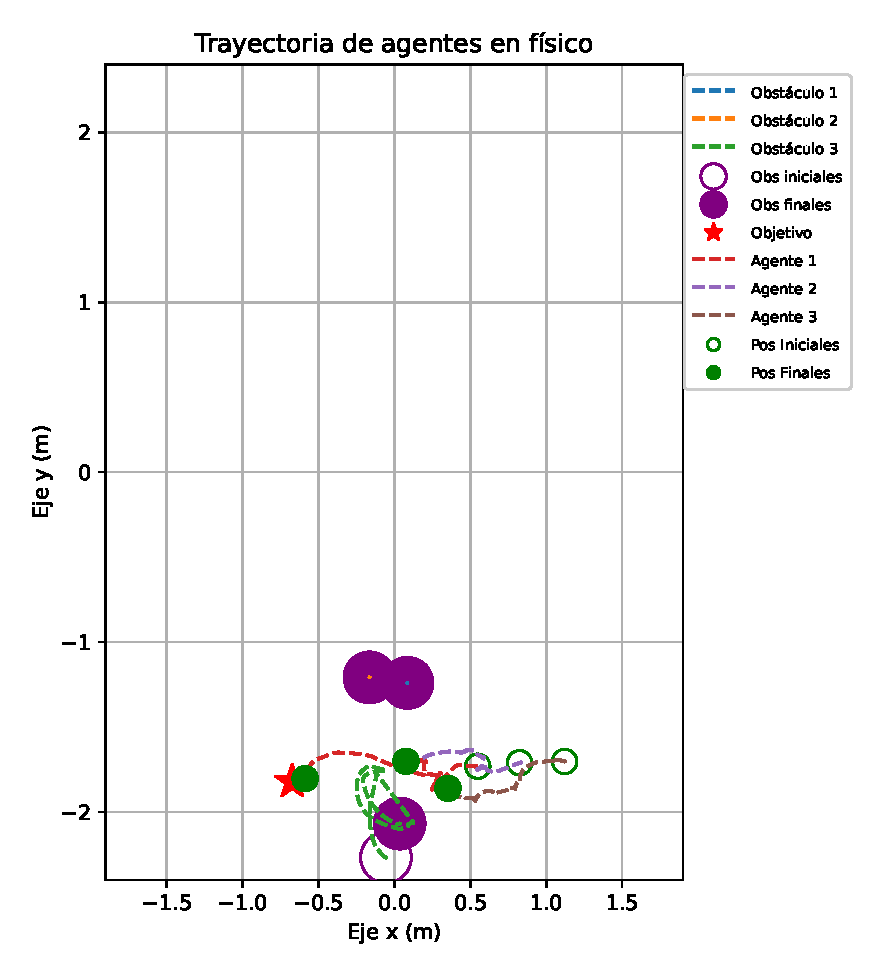
\includegraphics[width=\textwidth]{test_fisico_ObsM/traj_test_3A_ADC_f_3.eps}
	\caption{Trayectoria de los 3 agentes en el escenario ADC, corrida 3, en físico.}
	\label{fig:traj_test_3A_ADC_f_3}
\end{figure}

\subsection{Cuarto escenario}
Para este escenario, se movilizó el obstáculo una sola vez a manera que cambiara de posición e interfiriera con una trayectoria en línea recta de la formación hacia el objetivo. En la Figura \ref{fig:traj_test_3A_ADC_f_2}, se observa que los agentes modificaron su trayectoria evadiendo el obstáculo por un costado y siguieron exitosamente su camino hacia el objetivo.

\begin{figure}[H]
	\centering
	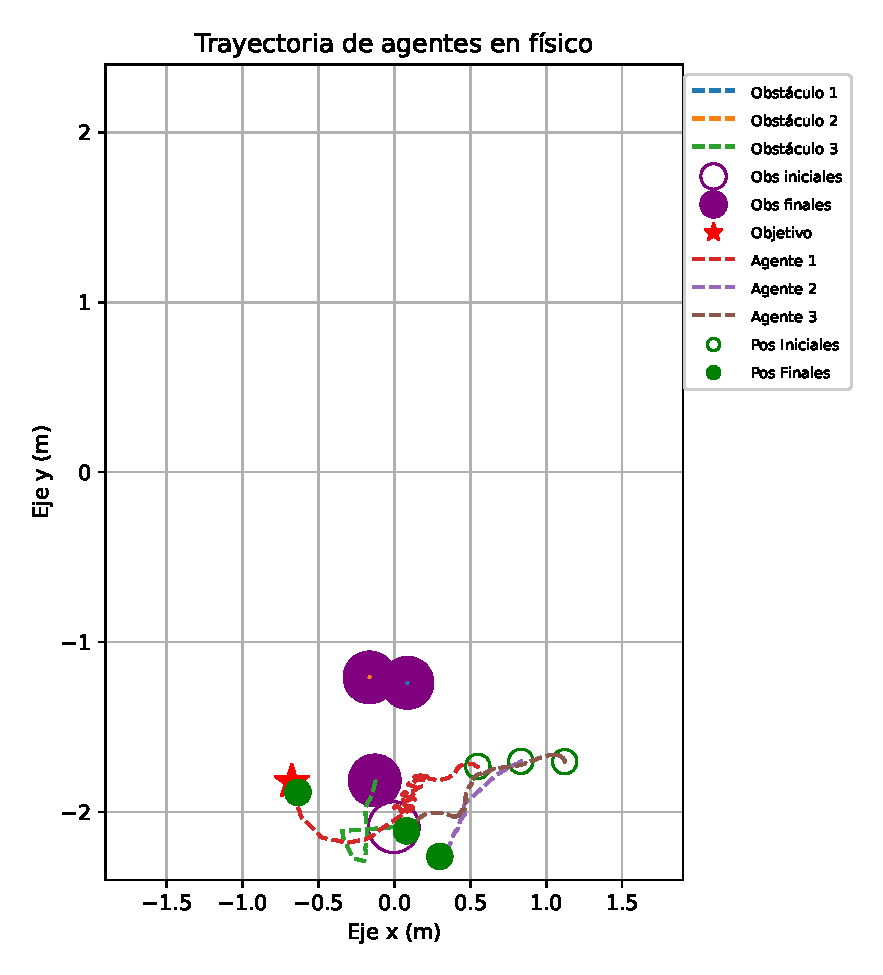
\includegraphics[width=\textwidth]{test_fisico_ObsM/traj_test_3A_ADC_f_2.eps}
	\caption{Trayectoria de los 3 agentes en el escenario ADC, corrida 2, en físico.}
	\label{fig:traj_test_3A_ADC_f_2}
\end{figure}


\chapter{Optimización del algoritmo y su implementación}\label{cap:optimizacion}
En este capítulo se describen los puntos de mejora identificados en la implementación del algoritmo de sincronización y control de formaciones. Además, se detalla cómo se abordó cada uno de ellos empleando técnicas de optimización como la reducción de complejidad computacional, paralelización y ajuste de parámetros de control. Por último, se compara el rendimiento del algoritmo con su implementación original y su versión optimizada.

\section{Lenguaje de programación y limpieza de código}
El primer paso para la optimización fue analizar el lenguaje de programación empleado para los controladores. Se tomó en cuenta tres lenguajes y se compararon con base en a las ventajas y desventajas que proponen para su implementación con el estado actual del algoritmo: MATLAB, Python y C. En el Cuadro \ref{cuadro:lenguajes_programacion} se describen las ventajas y desventajas de cada uno.

\begin{table}[H]
	\centering
	\resizebox{\textwidth}{!} {
	\begin{tabular}{|l|l|l|}
		\hline
		Lenguaje & Ventajas                                                                                                                                                                                                                                                                                                     & Desventajas                                                                                                                                                                                                                                                                                                             \\ \hline
		MATLAB   & \begin{tabular}[c]{@{}l@{}}- Es fácil de usar para simulaciones y prototipos.\\ \\ - Tiene una amplia variedad de herramientas \\ matemáticas.\\ \\ - Es excelente para algoritmos que involucran \\ operaciones matriciales.\end{tabular}                                                                      & \begin{tabular}[c]{@{}l@{}}- Es un lenguaje propio de MATLAB por lo que requiere comprar \\ licencias de software.\\ \\ - Su eficiencia computacional es menor en cuanto a rendimiento \\ comparado con Python o C.\end{tabular}                                                                                          \\ \hline
		Python   & \begin{tabular}[c]{@{}l@{}}- Es un lenguaje de código abierto.\\ \\ - Tiene una amplia variedad de librerías para optimizar \\ el cálculo numérico como NumPy, SciPy, multithreading \\ o multiprocessing.\\ \\ - Tiene un buen equilibrio entre rendmiento \\ computacional y facilidad de desarrollo.\end{tabular} & \begin{tabular}[c]{@{}l@{}}- Es un lenguaje más eficiente que MATLAB pero menos eficiente \\ que C debido a que es un lenguaje interpretado.\\ \\ - Requiere dependencias externas para lograr un alto rendimiento \\ (como integraciones con C).\end{tabular}                                                            \\ \hline
		C        & \begin{tabular}[c]{@{}l@{}}- Tiene un rendimiento superior ya que es un lenguaje \\ compilado de bajo nivel.\\ \\ - Ofrece un control sobre la memoria y el hardware.\end{tabular}                                                                                                                             & \begin{tabular}[c]{@{}l@{}}- Su complejidad es mucho mayor en cuando a implementación y \\ mantenimiento.\\ \\ - Tiene una alta probabilidad de fugas de memoria. \\ \\ - Requiere mucho más tiempo de desarrollo y es menos intuitivo.\\ \\ - No es tan flexible para realizar cambios rápidos en algoritmos.\end{tabular} \\ \hline
	\end{tabular}}
	\caption{Ventajas y desventajas de lenguajes de programación \cite{MatlabVsPython}.}
	\label{cuadro:lenguajes_programacion}
\end{table}

Una vez comparados los lenguajes de programación se optó por seguir utilizando Python para el desarrollo de los controladores. Las razones principales fueron que es un lenguaje de código abierto y ofrece un buen equilibrio entre rendimiento computacional y facilidad de desarrollo. Además, ya se cuenta con todo el algoritmo previo desarrollado en Python funcionando en un entorno físico como el Robotat. Esto incluye el desarrollo de los controladores, funciones para cálculos propios del algoritmo de sincronización y control de formaciones y funciones de conexión con el servidor del Robotat y los Pololu 3Pi+. Por lo que, dado el poco tiempo disponible para utilizar el Robotat no era conveniente migrar a un nuevo lenguaje de programación para esta fase de la implementación del algoritmo. Asimismo, Python cuenta con librerías como NumPy que está basada en C y otras librerías de comunicación y procesamiento que permiten optimizar el rendimiento computacional \cite{PythonVsC}.

Finalmente, se realizó un proceso de limpieza y documentación del código para facilitar la interacción y entendimiento. Además, esto permitió eliminar segmentos de código obsoletos, así como identificar otras deficiencias que se mencionarán a continuación.

\section{Posición de cada agente según el grafo de formación}
Durante la verificación de funcionalidad del algoritmo, al implementar la selección manual de marcadores para los agentes, se encontró que el número de marcador asignado a cada agente estaba directamente relacionado con la posición que este debe tomar según el grafo de formación. En la Figura \ref{fig:grafo_formacion1} se muestra la asignación de posiciones según el grafo de formación en triángulo para una selección arbitraria de agentes con la implementación original del algoritmo.

\begin{figure}[H]
	\centering
	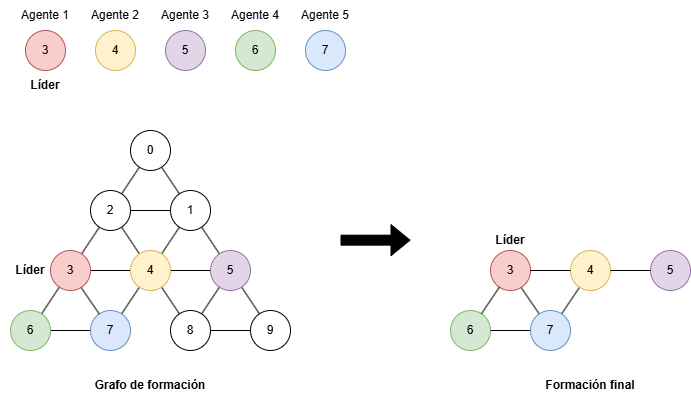
\includegraphics[width=0.8\textwidth]{optimizacion/grafo_formacion1.png}
	\caption{Posiciones de agentes según el grafo de formación con la implementación original del algoritmo.}
	\label{fig:grafo_formacion1}
\end{figure}

Al observar esto, se decidió optimizar la asignación de posición de cada agente a manera que siempre se mantenga la misma estructura del grafo de formación desde la posición cero y los agentes se posicionen de manera ascendente sin importar su número de marcador asignado, tal como se observa en la figura \ref{fig:grafo_formacion2}.

\begin{figure}[H]
	\centering
	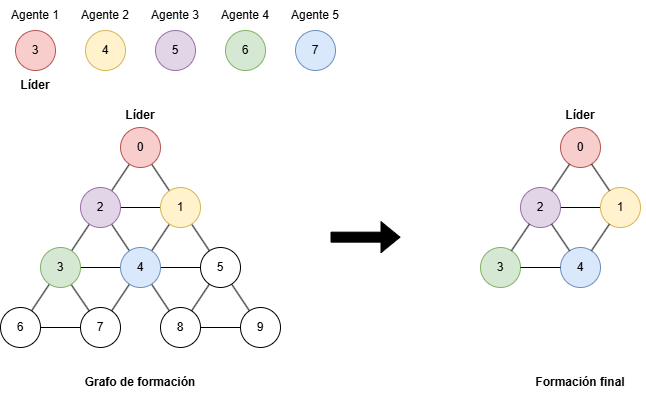
\includegraphics[width=0.8\textwidth]{optimizacion/grafo_formacion2.png}
	\caption{Posiciones de agentes según el grafo de formación con la implementación nueva del algoritmo.}
	\label{fig:grafo_formacion2}
\end{figure}

La versión optimizada vuelve al sistema consistente y robusto, independientemente del grupo de agentes seleccionado. Al estandarizar el proceso de selección de posiciones, se facilita tanto el diseño como la depuración. Además, es un sistema escalable, ya que la estructura fija de la formación permite la integración y reducción de agentes de forma sencilla y ordenada. Asimismo, incorpora un esquema eficiente para sistemas con múltiples agentes, donde las decisiones en tiempo real se simplifican gracias a una lógica más sencilla para gestionar las posiciones de los agentes en la formación.

\section{Mejora de la eficiencia computacional con NumPy}
NumPy es una librería de Python especializada para el cálculo numérico y científico. Destaca por su soporte para trabajar con operaciones vectorizadas o vectores multidimensionales sin realizar bucles. También cuenta con una amplia variedad de funciones matemáticas y estadísticas, así como integración con otras librerías como SciPy. Además, NumPy está implementado en C por lo que permite mejorar la eficiencia computacional para grandes cantidades de datos.

Al revisar los programas de los controladores, se encontró varios segmentos de código que se realizan con bucles (ciclos \textit{for}) simples y otros anidados. Esto representa una deficiencia al realizar los cálculos y solicitud de datos al servidor del Robotat, además que vuelve más compleja la depuración del programa, por lo que se decidió optimizar dichos procesos utilizando funciones matemáticas y operaciones matriciales con NumPy. A continuación, se detallará los segmentos del algoritmo que se optimizaron implementando operaciones con NumPy y se mostrará la comparativa en cuanto a tiempos de ejecución utilizando análisis estadísticos y la función ``perf\_counter\_ns'' de la librería ``time'' de Python, que permite medir tiempos en nanosegundos de manera precisa y luego realizar la conversión a otras unidades según sea necesario.

\subsection{Aplicación de desfases a los marcadores}
A continuación se explica los pasos que anteriormente se realizaban para aplicar los desfases de la calibración de marcadores, donde $n$ es la cantidad de marcadores a utilizar.

\begin{itemize}
	\item Configuración
	\begin{enumerate}
		\item Cargar el archivo .npy con los desfases de los marcadores.
		\item Solicitar las poses de $n$ marcadores al sevidor del Robotat.
		\item Aplicar el desfase de cada marcador con un bucle de $n$ iteraciones.
	\end{enumerate}
	\item Ciclo principal 
	\begin{enumerate}
		\item Solicitar las poses de $n$ marcadores al servidor del Robotat.
		\item Aplicar el desfase de cada marcador con un bucle de $n$ iteraciones.
	\end{enumerate}
\end{itemize}

Implementar bucles dentro del ciclo principal significa un aumento de tiempo computacional que es más notorio al aumentar la cantidad de marcadores a utilizar. Para optimizar el proceso se optó por aplicar los desfases a cada marcador utilizando operaciones matriciales e implementando únicamente una resta de matrices dentro del ciclo principal, por lo que ahora el proceso es el siguiente:

\begin{itemize}
	\item Configuración
	\begin{enumerate}
		\item Cargar el archivo .npy con los desfases de los marcadores.
		\item Almacenar los desfases en la cuarta columna de una matriz de ceros de tamaño $n \times 6$.
		\item Solicitar las poses de los marcadores al sevidor del Robotat.
		\item Aplicar el desfase de los marcadores con una resta de la matriz con los desfases a la matriz con las poses de los marcadores.
	\end{enumerate}
	\item Ciclo principal 
	\begin{enumerate}
		\item Solicitar las poses de los marcadores al servidor del Robotat.
		\item Aplicar el desfase de los marcadores con una resta de la matriz con los desfases a la matriz con las poses de los marcadores.
	\end{enumerate}
\end{itemize}

Una vez implementada la optimización, se realizó un análisis estadístico con mil muestras donde se tomó el tiempo que toma aplicar los desfases a los marcadores con bucles y con una resta de matrices con NumPy.

Para la toma de muestras, se evaluaron diferentes cantidades de marcadores a los que se les aplicó el desfase, siendo estos 5, 10, 15 y 20. En los Cuadros \ref{cuadro:tiempos_desfases_for} y \ref{cuadro:tiempos_desfases_numpy} se muestran la media y desviación estándar del tiempo que tomó aplicar los desfases.

En la Figura \ref{fig:grafica_tiempos_desfases} se observa que la optimización con NumPy presenta una reducción notable en el tiempo de procesamiento, la cual es aún más significativa a medida que aumenta la cantidad de marcadores a utilizar. Por otro lado, los tiempos al aplicar bucles incrementan de manera proporcional y más pronunciada con el aumento de los marcadores, mientras que con NumPy el crecimiento es más moderado ya que la pendiente de la curva es dos órdenes de magnitud menor.

Finalmente, en el Cuadro \ref{cuadro:tiempo_reducido_desfases} se presentan los resultados de la reducción de tiempo lograda con la versión optimizada con NumPy. La mayor reducción se obtuvo al aplicar el desfase a $20$ marcadores, alcanzando una disminución de $9.648$ microsegundos.

\begin{table}[H]
	\centering
	\resizebox{\textwidth}{!} {
	\begin{tabular}{|l|l|l|l|}
		\hline
		\textbf{Cantidad de marcadores} & \textbf{Número de muestras} & \textbf{Media de tiempo (us)} & \textbf{Desviación estándar (us)} \\ \hline
		5                               & 1000                        & 2.802                         & 0.308                             \\ \hline
		10                              & 1000                        & 5.353                         & 0.469                             \\ \hline
		15                              & 1000                        & 8.187                         & 1.654                             \\ \hline
		20                              & 1000                        & 10.485                        & 0.843                             \\ \hline
	\end{tabular}}
	\caption{Media de tiempo y desviación estándar para aplicar desfases de marcadores con bucles.}
	\label{cuadro:tiempos_desfases_for}
\end{table}

\begin{table}[H]
	\centering
	\resizebox{\textwidth}{!} {
	\begin{tabular}{|l|l|l|l|}
		\hline
		\textbf{Cantidad de marcadores} & \textbf{Número de muestras} & \textbf{Media de tiempo (us)} & \textbf{Desviación estándar (us)} \\ \hline
		5                               & 1000                        & 0.734                         & 0.119                             \\ \hline
		10                              & 1000                        & 0.756                         & 0.113                             \\ \hline
		15                              & 1000                        & 0.794                         & 0.225                             \\ \hline
		20                              & 1000                        & 0.837                         & 0.147                             \\ \hline
	\end{tabular}}
	\caption{Media de tiempo y desviación estándar para aplicar desfases de marcadores con NumPy.}
	\label{cuadro:tiempos_desfases_numpy}
\end{table}

\begin{table}[H]
	\centering
	\resizebox{0.5\textwidth}{!} {
	\begin{tabular}{|l|l|}
		\hline
		\textbf{Cantidad de marcadores} & \textbf{Tiempo reducido (us)} \\ \hline
		5                               & 2.068                         \\ \hline
		10                              & 4.597                         \\ \hline
		15                              & 7.393                         \\ \hline
		20                              & 9.648                         \\ \hline
	\end{tabular}}
	\caption{Tiempo reducido al aplicar los desfases de marcadores utilizando NumPy.}
	\label{cuadro:tiempo_reducido_desfases}
\end{table}

\begin{figure}[H]
	\centering
	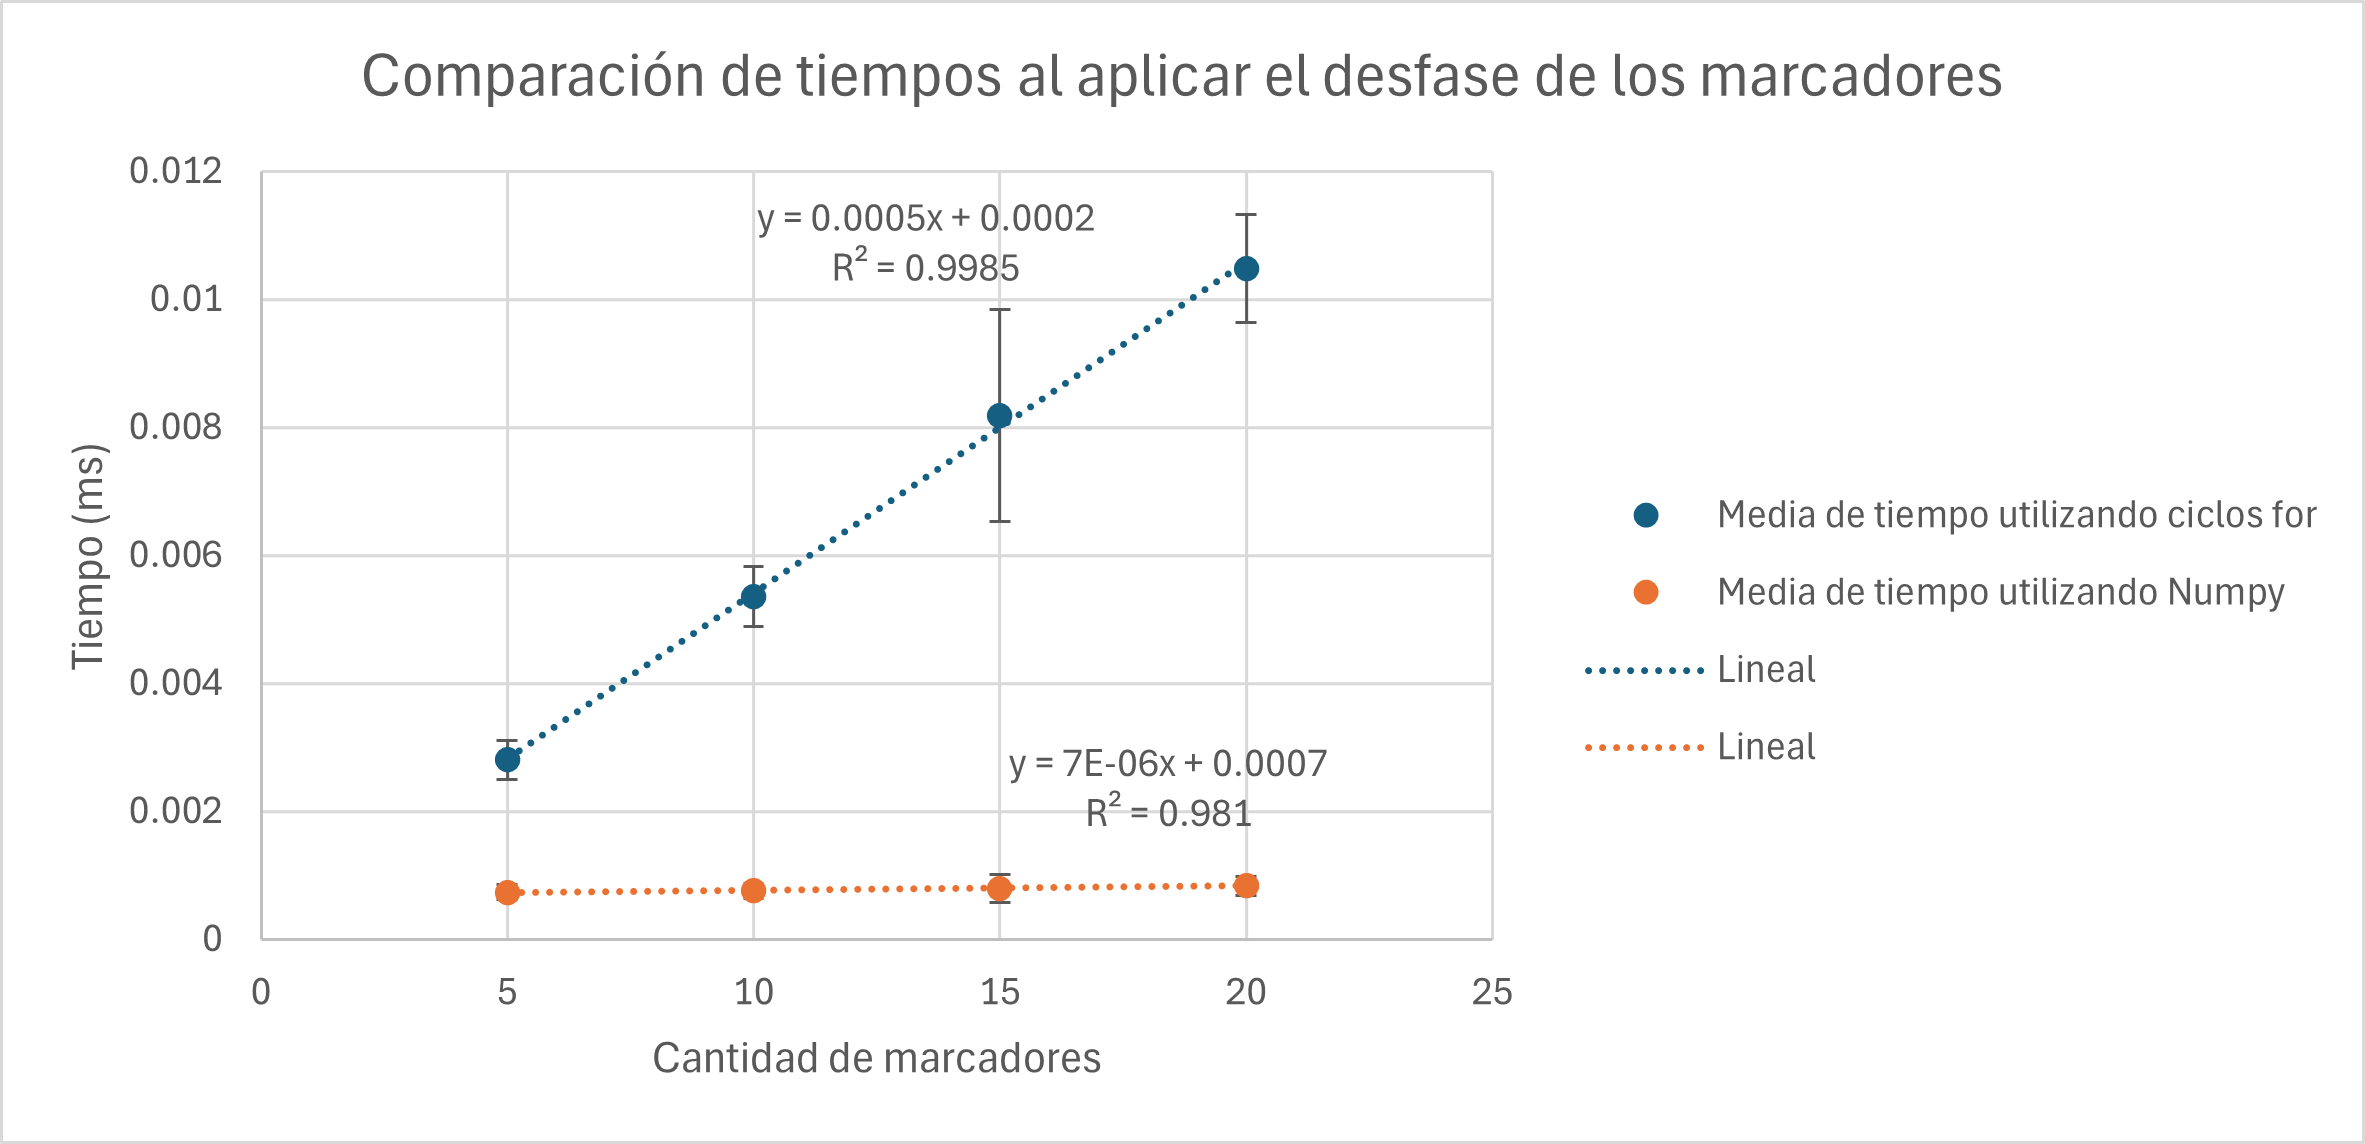
\includegraphics[width=\textwidth]{optimizacion/tiempos_desfases.png}
	\caption{Gráfica con medias de tiempo para aplicar desfases de marcadores con bucles y operaciones con NumPy.}
	\label{fig:grafica_tiempos_desfases}
\end{figure}

\subsection{Cálculo de la distancia entre agentes}
Para el cálculo de distancia entre agentes se tenía una función llamada ``DistBetweenAgents'' dentro del archivo ``funciones.py''. Esta utilizaba bucles anidados para calcular la norma de distancia basada en la distancia en $x$ y $y$ de cada agente hacia sus vecinos más próximos. El cálculo de la distancia se realiza entre los agentes $i$ y $j$ y luego para $j$ e $i$, esto produce una matriz simétrica por lo que se puede realizar únicamente el cálculo de una mitad y luego duplicarla. Para esto, se creó una versión optimizada de la función llamada ``DistBetweenAgentsOptimized''. En esta, únicamente se calcula la diferencia de posiciones aprovechando el \textit{broadcasting} en NumPy y luego se obtiene la norma de la matriz de distancias utilizando la función ``linealg.norm''.

En los Cuadros \ref{cuadro:tiempos_distancias_for} y \ref{cuadro:tiempos_distancias_numpy} se muestran la media y desviación estándar del tiempo que toma en realizar los cálculos con la función original y la optimizada. Para esto, se tomó mil muestras aumentando la cantidad de agentes desde $1$ hasta $10$. 

En la Figura \ref{fig:grafica_tiempos_distancias} se observa un incremento exponencial en el tiempo de procesamiento al calcular las distancias entre los agentes conforme se aumenta el número de estos en la formación. Además, la optimización con NumPy presenta un incremento significativamente menor. Esto se confirma al observar que el exponente de la ecuación que describe el comportamiento utilizando bucles es $1.6982$, mientras que el exponente al utilizar NumPy es $0.1775$.

Finalmente, en el Cuadro \ref{cuadro:tiempo_reducido_distancia} se presentan los resultados de la reducción de tiempo lograda con la versión optimizada utilizando NumPy. Aunque la reducción de tiempo comienza a partir de los $3$ agentes, el ligero aumento de tiempo al utilizar NumPy con $1$ y $2$ agentes no fue significativo. La mayor reducción de tiempo se obtuvo al calcular la distancia con $10$ agentes, alcanzando una disminución de $88.705$ microsegundos.

\begin{table}[H]
	\centering
	\resizebox{\textwidth}{!} {
	\begin{tabular}{|l|l|l|l|}
		\hline
		\textbf{Cantidad de marcadores} & \textbf{Número de muestras} & \textbf{Media de tiempo (us)} & \textbf{Desviación estándar (us)} \\ \hline
		1                               & 1000                        & 2.130                         & 0.343                             \\ \hline
		2                               & 1000                        & 5.569                         & 6.185                             \\ \hline
		3                               & 1000                        & 9.883                         & 0.914                             \\ \hline
		4                               & 1000                        & 16.406                        & 1.267                             \\ \hline
		5                               & 1000                        & 26.257                        & 5.967                             \\ \hline
		6                               & 1000                        & 36.697                        & 7.060                             \\ \hline
		7                               & 1000                        & 51.342                        & 3.965                             \\ \hline
		8                               & 1000                        & 62.752                        & 12.055                            \\ \hline
		9                               & 1000                        & 79.696                        & 9.144                             \\ \hline
		10                              & 1000                        & 98.319                        & 9.456                             \\ \hline
	\end{tabular}}
	\caption{Media de tiempo y desviación estándar para calcular la distancia entre agentes con bucles.}
	\label{cuadro:tiempos_distancias_for}
\end{table}

\begin{table}[H]
	\centering
	\resizebox{\textwidth}{!} {
	\begin{tabular}{|l|l|l|l|}
		\hline
		\textbf{Cantidad de marcadores} & \textbf{Número de muestras} & \textbf{Media de tiempo (us)} & \textbf{Desviación estándar (us)} \\ \hline
		1                               & 1000                        & 6.100                         & 1.477                             \\ \hline
		2                               & 1000                        & 8.134                         & 1.457                             \\ \hline
		3                               & 1000                        & 8.187                         & 7.005                             \\ \hline
		4                               & 1000                        & 8.354                         & 6.599                             \\ \hline
		5                               & 1000                        & 8.918                         & 1.580                             \\ \hline
		6                               & 1000                        & 8.835                         & 1.695                             \\ \hline
		7                               & 1000                        & 9.344                         & 1.726                             \\ \hline
		8                               & 1000                        & 9.559                         & 4.158                             \\ \hline
		9                               & 1000                        & 9.581                         & 2.898                             \\ \hline
		10                              & 1000                        & 9.614                         & 2.514                             \\ \hline
	\end{tabular}}
	\caption{Media de tiempo y desviación estándar para calcular la distancia entre agentes con NumPy.}
	\label{cuadro:tiempos_distancias_numpy}
\end{table}

\begin{table}[H]
	\centering
	\resizebox{0.5\textwidth}{!} {
	\begin{tabular}{|l|l|}
		\hline
		\textbf{Cantidad de marcadores} & \textbf{Tiempo reducido (us)} \\ \hline
		1                               & -3.970                        \\ \hline
		2                               & -2.565                        \\ \hline
		3                               & 1.696                         \\ \hline
		4                               & 8.052                         \\ \hline
		5                               & 17.339                        \\ \hline
		6                               & 27.862                        \\ \hline
		7                               & 41.998                        \\ \hline
		8                               & 53.193                        \\ \hline
		9                               & 70.115                        \\ \hline
		10                              & 88.705                        \\ \hline
	\end{tabular}}
	\caption{Tiempo reducido al calcular la distancia entre agentes utilizando NumPy.}
	\label{cuadro:tiempo_reducido_distancia}
\end{table}

\begin{figure}[H]
	\centering
	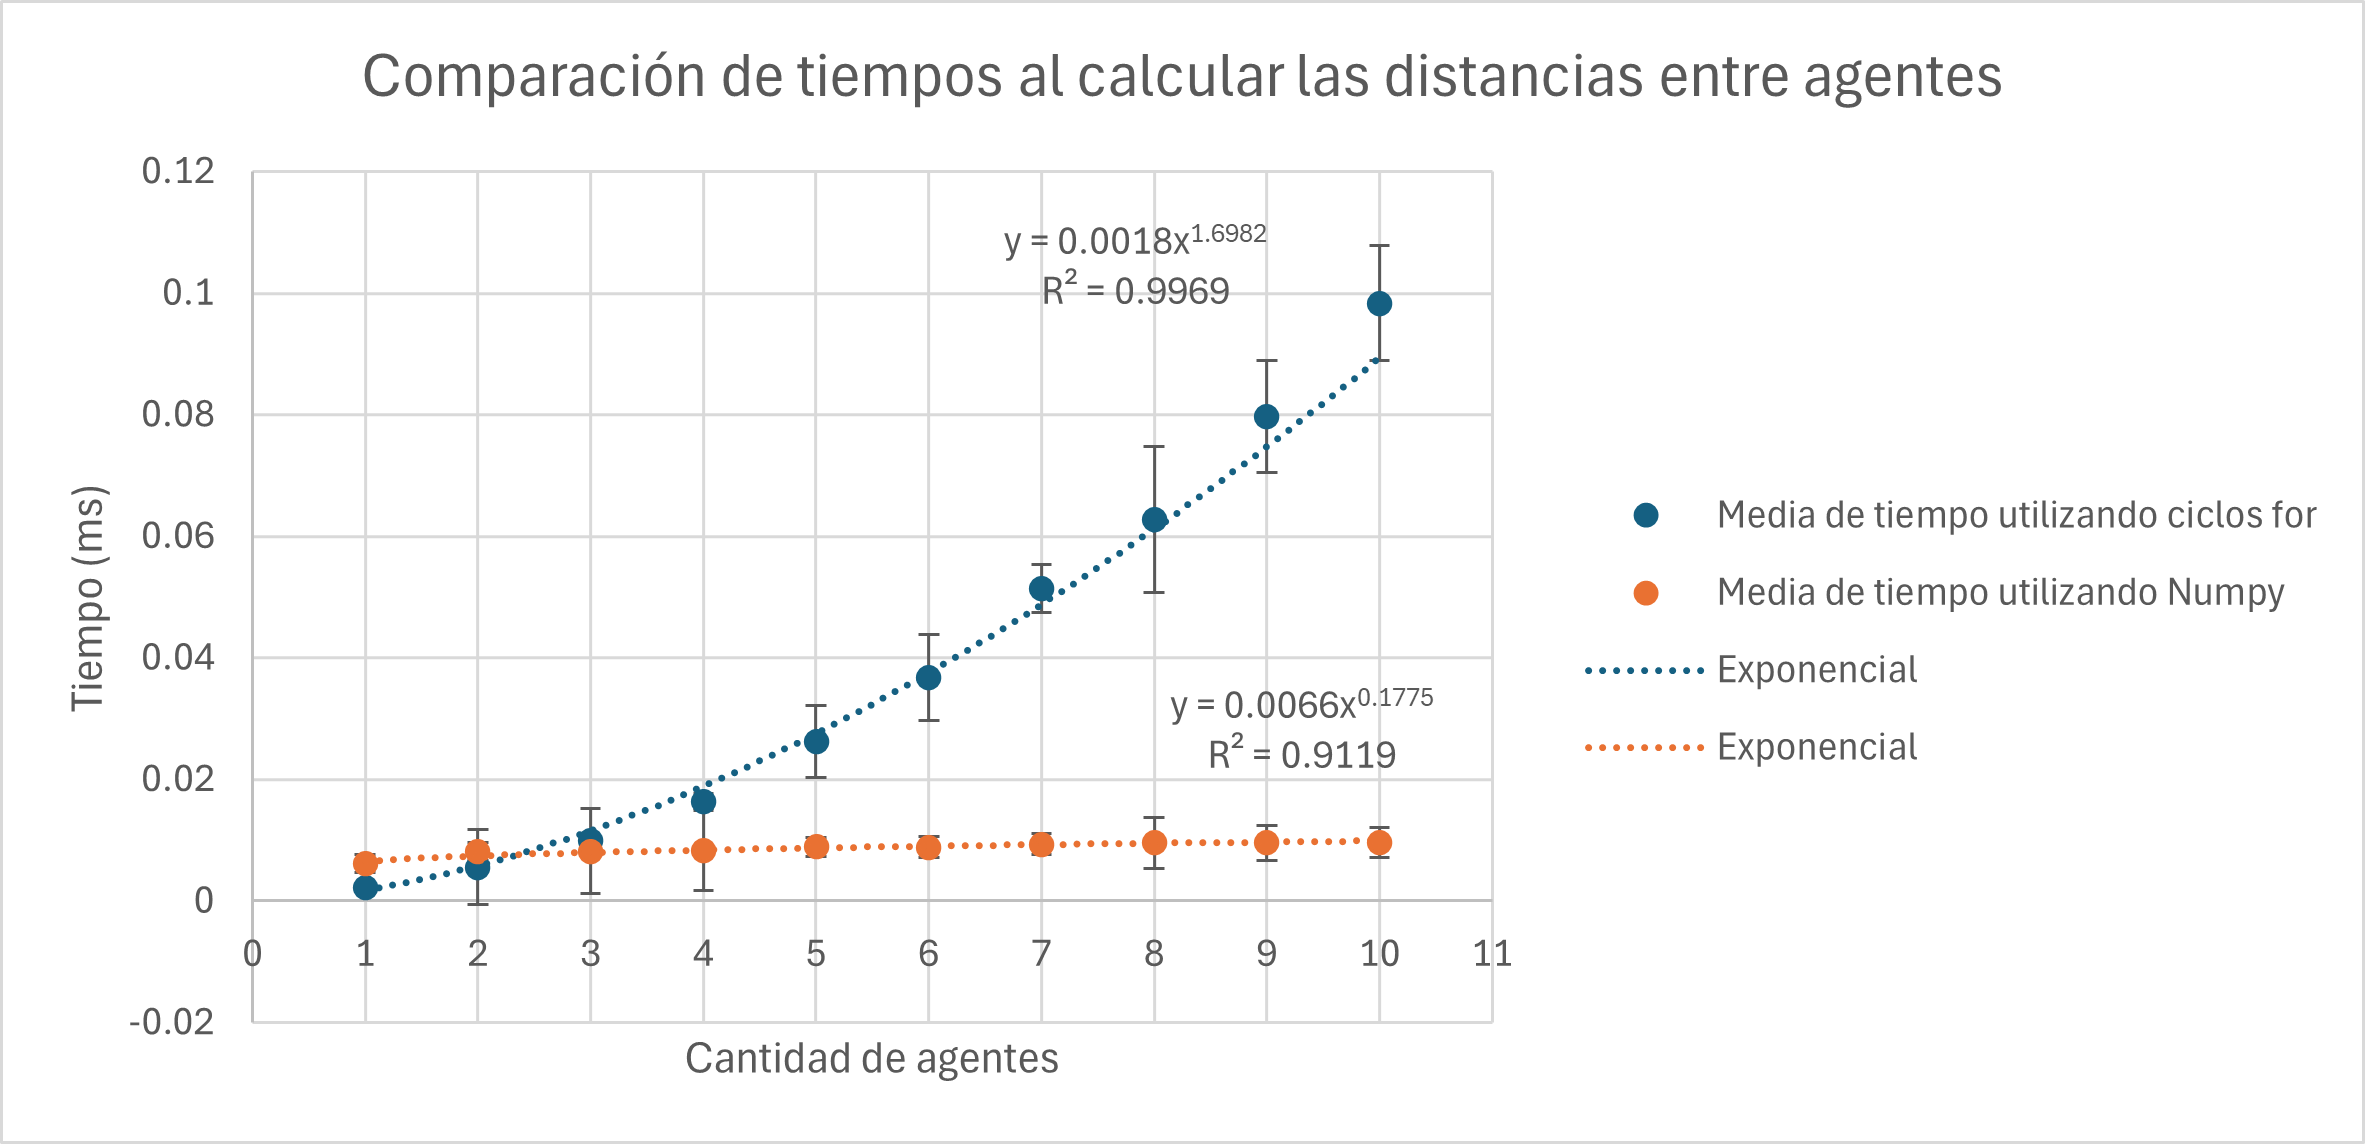
\includegraphics[width=\textwidth]{optimizacion/tiempos_distancias.png}
	\caption{Gráfica con medias de tiempo para calcular la distancia entre agentes con bucles y operaciones con NumPy.}
	\label{fig:grafica_tiempos_distancias}
\end{figure}

\subsection{Cálculo del error de formación}
Para calcular el error de formación se utilizaba la función ``FormationError'' dentro del archivo ``funciones.py''. Esta función utiliza dos bucles anidados para calcular el error cuadrático medio entre la formación actual y la deseada utilizando como parámetros las matrices de adyacencia de ambas formaciones. Dado que ambas matrices son cuadradas y, al considerar únicamente los agentes de interés, se convierten en matrices del mismo tamaño, se desarrolló una versión optimizada de la función llamada ``FormationErrorOptimized''. Esta versión emplea la función ``square'' de NumPy que eleva al cuadrado cada elemento de la matriz y luego calcula la media utilizando la función ``mean''.

En los Cuadros \ref{cuadro:tiempos_error_for} y \ref{cuadro:tiempos_error_numpy} se muestran la media y desviación estándar del tiempo que toma en realizar el cálculo del error cuadrático medio con la función original y la optimizada. Para esto, se tomó mil muestras aumentando la cantidad de agentes desde $1$ hasta $10$. 

En la Figura \ref{fig:grafica_tiempos_error} se muestra una gráfica en la que se evidencia un crecimiento exponencial en el tiempo de procesamiento al calcular las distancias entre los agentes a medida que se aumenta el número de agentes en la formación. Por otro lado, la optimización con Numpy, presenta un aumento significativamente menor. Además, esto se demuestra ya que el exponente de la ecuación que describe el comportamiento utilizando bucles es $1.4753$, mientras que el exponente para la optimización con NumPy es $0.112$.

Finalmente, en el Cuadro \ref{cuadro:tiempo_reducido_error} se presentan los resultados de la reducción de tiempo lograda con la versión optimizada utilizando NumPy. Aunque la reducción de tiempo comienza a partir de los $4$ agentes, el aumento de tiempo al utilizar NumPy con $1$, $2$ y $3$ agentes no fue significativo. La mayor reducción de tiempo se obtuvo al calcular el error de formación con $10$ agentes, alcanzando una disminución de $127.378$ microsegundos.

\begin{table}[H]
	\centering
	\resizebox{\textwidth}{!} {
	\begin{tabular}{|l|l|l|l|}
		\hline
		\textbf{Cantidad de marcadores} & \textbf{Número de muestras} & \textbf{Media de tiempo (us)} & \textbf{Desviación estándar (us)} \\ \hline
		1                               & 1000                        & 5.665                         & 0.809                             \\ \hline
		2                               & 1000                        & 11.010                        & 0.895                             \\ \hline
		3                               & 1000                        & 18.721                        & 8.085                             \\ \hline
		4                               & 1000                        & 29.093                        & 7.140                             \\ \hline
		5                               & 1000                        & 43.071                        & 3.761                             \\ \hline
		6                               & 1000                        & 58.559                        & 8.292                             \\ \hline
		7                               & 1000                        & 75.147                        & 10.952                            \\ \hline
		8                               & 1000                        & 103.554                       & 8.648                             \\ \hline
		9                               & 1000                        & 128.032                       & 11.905                            \\ \hline
		10                              & 1000                        & 149.833                       & 13.256                            \\ \hline
	\end{tabular}}
	\caption{Media de tiempo y desviación estándar para calcular el error de formación con bucles.}
	\label{cuadro:tiempos_error_for}
\end{table}

\begin{table}[H]
	\centering
	\resizebox{\textwidth}{!} {
	\begin{tabular}{|l|l|l|l|}
		\hline
		\textbf{Cantidad de marcadores} & \textbf{Número de muestras} & \textbf{Media de tiempo (us)} & \textbf{Desviación estándar (us)} \\ \hline
		1                               & 1000                        & 16.538                        & 7.916                             \\ \hline
		2                               & 1000                        & 20.229                        & 2.389                             \\ \hline
		3                               & 1000                        & 20.081                        & 3.186                             \\ \hline
		4                               & 1000                        & 20.134                        & 3.423                             \\ \hline
		5                               & 1000                        & 20.714                        & 3.501                             \\ \hline
		6                               & 1000                        & 21.065                        & 4.530                             \\ \hline
		7                               & 1000                        & 21.143                        & 5.589                             \\ \hline
		8                               & 1000                        & 22.082                        & 3.146                             \\ \hline
		9                               & 1000                        & 22.348                        & 4.730                             \\ \hline
		10                              & 1000                        & 22.455                        & 24.888                            \\ \hline
	\end{tabular}}
	\caption{Media de tiempo y desviación estándar para calcular el error de formación con NumPy.}
	\label{cuadro:tiempos_error_numpy}
\end{table}

\begin{table}[H]
	\centering
	\resizebox{0.5\textwidth}{!} {
	\begin{tabular}{|l|l|}
		\hline
		\textbf{Cantidad de marcadores} & \textbf{Tiempo reducido (us)} \\ \hline
		1                               & -10.873                       \\ \hline
		2                               & -9.219                        \\ \hline
		3                               & -1.360                        \\ \hline
		4                               & 8.959                         \\ \hline
		5                               & 22.357                        \\ \hline
		6                               & 37.494                        \\ \hline
		7                               & 54.004                        \\ \hline
		8                               & 81.472                        \\ \hline
		9                               & 105.684                       \\ \hline
		10                              & 127.378                       \\ \hline
	\end{tabular}}
	\caption{Tiempo reducido al calcular el error de formación utilizando NumPy.}
	\label{cuadro:tiempo_reducido_error}
\end{table}

\begin{figure}[H]
	\centering
	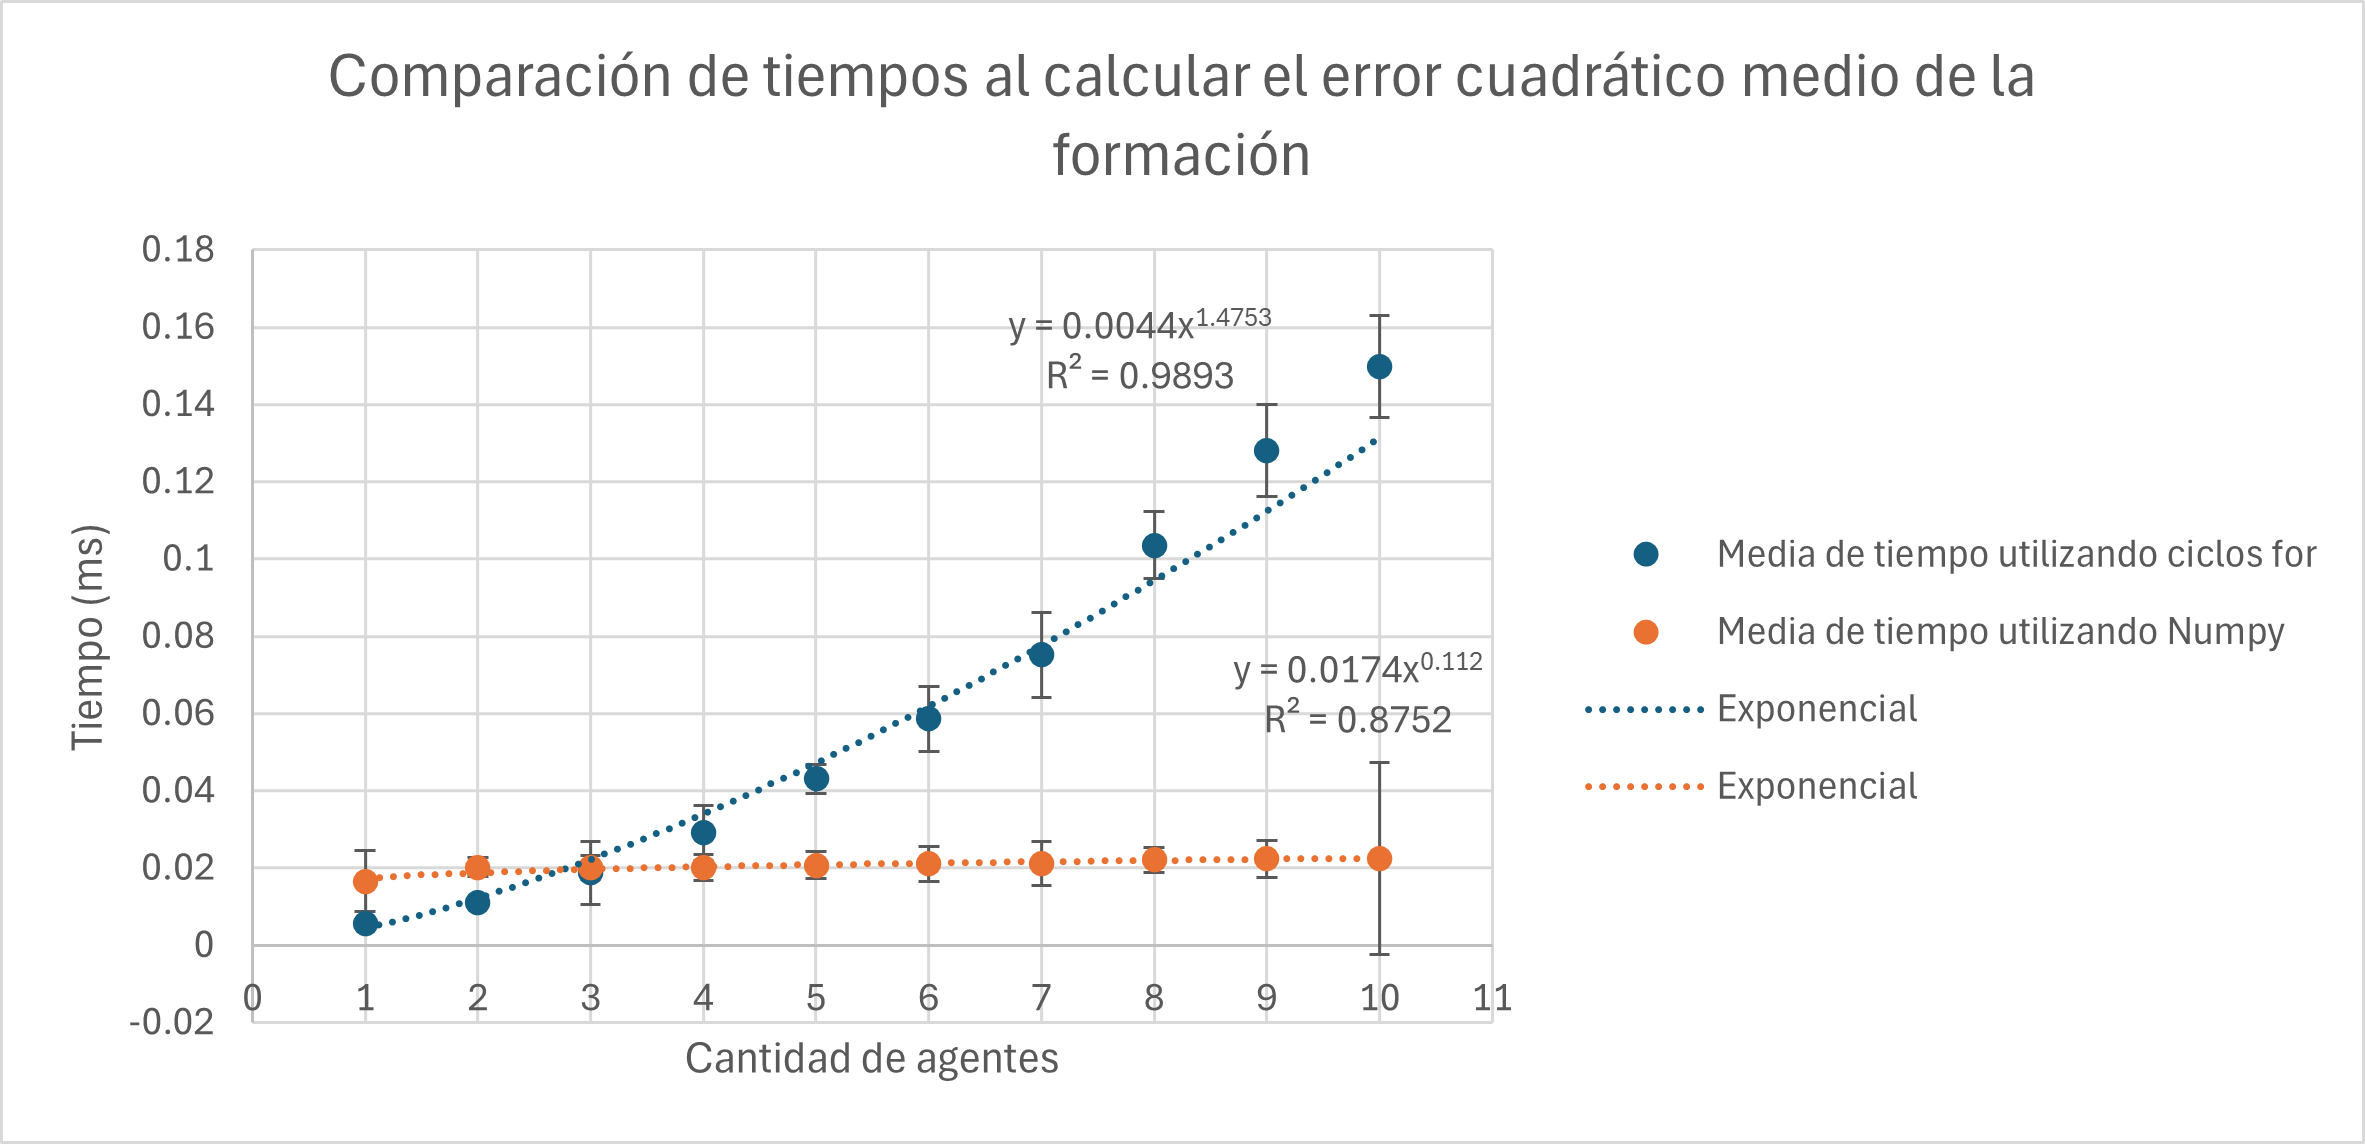
\includegraphics[width=\textwidth]{optimizacion/tiempos_error.png}
	\caption{Gráfica con medias de tiempo para calcular el error de formación con bucles y operaciones con NumPy.}
	\label{fig:grafica_tiempos_error}
\end{figure}

\section{Implementación de paralelismo computacional}
En este capítulo, se explica cómo se modificó el programa para implementar paralelismo computacional utilizando hilos con la librería ``threading'' de Python.

\subsection{Definición de funcionalidades que se ejecutarán en paralelo}
El primer paso fue definir las secciones del programa que se pueden ejecutar en paralelo de manera autónoma sin depender de estados externos o recursos no sincronizados. Estas secciones fueron:
\begin{itemize}
	\item El algoritmo de sincronización y control de formaciones.
	\item El proceso de obtener las poses de los marcadores del Robotat.
	\item La visualización en tiempo real con Webots del escenario físico.
\end{itemize}

Dado que el controlador del agente realiza operaciones secuenciales y cálculos de velocidades que dependen de más instancias, se decidió implementar hilos únicamente en el controlador del supervisor, en paralelo a la ejecución del algoritmo de sincronización y control de formaciones, tal como se observa en la Figura \ref{fig:hilos}.

\begin{figure}[H]
	\centering
	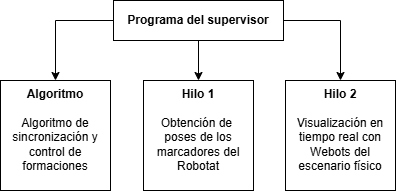
\includegraphics[width=0.5\textwidth]{optimizacion/paralelismo/diagrama_threading.png}
	\caption{Funcionalidades del algoritmo que se ejecutan en paralelo.}
	\label{fig:hilos}
\end{figure}

\subsection{Creación de hilos en paralelo}

Una vez identificadas las funcionalidades que se pueden ejecutar en paralelo, se definió la estructura de las tareas para cada hilo, tal como se observa en la Figura \ref{fig:diagrama_hilos}. 

Se implementó la ejecución de hilos en paralelo utilizando la librería ``threading'' de Python ya que resulta útil para manejar tareas que involucran tiempos de espera y no requieren una capacidad de procesamiento elevada \cite{PythonThreading}. En el caso de la obtención de las poses de los marcadores, es necesario un tiempo de espera entre la comunicación de la computadora y el servidor del Robotat. Este tiempo puede aprovecharse ejecutando otras tareas y cálculos esenciales del algoritmo en paralelo. Además, esto evita problemas de sincronización debido a los tiempos de espera altos por la latencia del servidor.

En cuanto a la visualización en tiempo real en Webots, inicialmente ya se contaba con esta funcionalidad implementada dentro del ciclo principal, sin embargo esta requiere recursos adicionales y se puede ejecutar en paralelo sin afectar al funcionamiento del algoritmo. Por esto, se agregó un hilo dedicado exclusivamente a la visualización en tiempo real del escenario en Webots. Adicionalmente, se implementó un evento de sincronización para garantizar que la visualización se mantenga en sincronía con cada paso de la simulación. Este evento se activa al inicio de cada ciclo del supervisor que ya se encuentra sincronizado con el paso de la simulación, y el hilo queda a la espera de recibir el evento para ejecutar las tareas.

Luego, para todos los hilos, se definió un evento de finalización que se activa cuando el líder llega al objetivo y el error de formación es menor al $10\%$. Finalmente, para terminar los hilos, se utilizó la función ``join'' de la librería ``threading'' para bloquear el programa principal y esperar a que cada hilo finalice de manera segura antes de detener el programa.


\begin{figure}[H]
	\centering
	\includegraphics[width=0.8\textwidth]{optimizacion/paralelismo/diagrama_threading_extendido.png}
	\caption{Funcionalidades del algoritmo que se ejecutan en paralelo.}
	\label{fig:diagrama_hilos}
\end{figure}

\section{Ajuste de parámetros y mejora de funcionalidades}
Durante la optimización del algoritmo, se encontró con nuevas oportunidades de mejora que se explican a continuación.

\subsection{Configuración del escenario y marcadores}
Anteriormente, era necesario configurar manualmente el listado de marcadores para los agentes tanto en el controlador del supervisor como en el de los agentes. De la misma manera, se requería especificar el modo de operación (físico o simulado) y la velocidad máxima para los agentes. Esto implicaba realizar modificaciones en ambos controladores cada vez que se realizaban cambios en las condiciones del escenario y los agentes.

Este enfoque ocasionaba problemas frecuentes, ya que a menudo se olvidaba actualizar ciertos parámetros en uno de los controladores, lo que complicaba la depuración y las pruebas. Para solucionar esto, se decidió implementar una memoria compartida adicional que centralizara las configuraciones en el controlador del supervisor. Dicha memoria se configuró para enviar parámetros como el modo de operación, la velocidad máxima de los agentes y el listado de marcadores a utilizar desde un único controlador. Esta solución no solo facilita la depuración y reduce la posibilidad de discrepancias en las configuraciones, sino que también proporciona un sistema más robusto y eficiente para la gestión de variables.

\subsection{Medición del tiempo de ejecución del algoritmo}
En la fase previa, no se tenía un sistema preciso para medir el tiempo de ejecución del algoritmo. En su lugar, se realizaba un cálculo aproximado basado en la cantidad de ciclos ejecutados y su conversión según el paso de tiempo configurado en la simulación. Sin embargo, este paso estaba fijado en $64$ milisegundos, mientras que cada ciclo en realidad tomaba más tiempo debido a la carga computacional del algoritmo y a la latencia de comunicación con el servidor dentro del ciclo principal, lo que generaba problemas de sincronización. 

Para resolver esta limitación, se implementó un sistema de medición precisa utilizando la función ``perf\_counter\_ns'' de la librería ``time'' que permite medir el tiempo en nanosegundos para luego realizar la conversión a segundos. Este sistema se implementó para medir el tiempo desde el momento en que los agentes ya se encuentran en sus posiciones iniciales hasta el final del experimento, que para esta fase se definió como el momento en que el líder se ubica a $20$ centímetros del objetivo y el error de formación es menor al $10\%$. Esta solución permitió obtener mediciones de tiempo exactas y fue implementada tanto en el algoritmo optimizado como en el no optimizado, facilitando así una comparación precisa del rendimiento entre ambas versiones.

\subsection{Visualización en tiempo real en Webots del escenario}
Como se mencionó anteriormente, inicialmente ya se contaba con esta funcionalidad pero solo se mostraba la posición de los obstáculos y el objetivo. Por esto, se decidió agregar la funcionalidad de visualización para los agentes. En la Figura \ref{visualizacion} se observa un escenario físico y su visualización en tiempo real en Webots con la siguiente representación:

\begin{itemize}
	\item Círculos verdes: posiciones iniciales para los agentes.
	\item Círculo amarillo: posición en tiempo real del agente líder de la formación.
	\item Círculos azules: posiciones en tiempo real de los demás agentes.
	\item Círculo rojo: posición en tiempo real del objetivo.
	\item Toroides morados: posiciones en tiempo real de los obstáculos.
	\item ePucks: posiciones en que se encontraban los agentes al momento de ejecutar el programa (antes de colocarse en sus posiciones iniciales).
\end{itemize}

\begin{figure}[H]
	\centering
	\includegraphics[width=0.45\textwidth]{/mejoras/real_time_v_fisico.JPEG}
	\includegraphics[width=0.45\textwidth]{/mejoras/real_time_v_webots.png}
	\caption{Visualización en tiempo real del escenario. A la izquierda está el escenario físico y a la derecha su visualización en tiempo real en Webots.}
	\label{fig:visualizacion}
\end{figure}

\subsection{Monitoreo de variables}
Por último, para monitorear el comportamiento del algoritmo durante su ejecución, se incorporó la visualización en tiempo real de los siguientes factores, los cuales se muestran en la terminal de Webots, como se observa en la Figura \ref{fig:variables}.

\begin{itemize}
	\item La etapa en la que se encuentra el algoritmo.
	\item La norma de velocidades sobre la cuál se toman decisiones en el algoritmo.
	\item El error de formación.
	\item La latencia de comunicación con el servidor del Robotat.
\end{itemize}

\begin{figure}[H]
	\centering
	\includegraphics[width=0.5\textwidth]{/mejoras/terminal.png}
	\caption{Monitoreo de variables en tiempo real con la terminal de Webots.}
	\label{fig:variables}
\end{figure}

\chapter{Verificación del rendimiento del algoritmo optimizado} \label{cap:verificacion_optim}
En este capítulo, se explica como se realizó la verificación del rendimiento del algoritmo optimizado realizando un total de $24$ experimentos, con el fin de comparar el tiempo de ejecución entre el algoritmo optimizado y el no optimizado.

\section{Configuración del escenario}
Una vez aplicadas todas las mejoras al algoritmo, se realizó la verificación de su rendimiento utilizando el escenario de la Figura \ref{fig:escenario_optimizacion}, que está definido de la siguiente manera:
\begin{itemize}
	\item Estrella roja: representa el objetivo y se encuentra a $1$ metro hacia arriba del centro del escenario.
	\item Círculos morados: representan los obstáculos y se encuentran sobre el eje $X$ al centro del escenario.
	\item Círculos verdes: representan las posiciones iniciales para los agentes. El primer agente (círculo verde más a la izquierda) se encuentra a $1$ metro por debajo del centro del escenario y $1.5$ metros a la izquierda. Las posiciones se ocupan de izquierda a derecha según la cantidad de agentes a utilizar y hay $15$ centímetros entre cada posición inicial.
\end{itemize}

\begin{figure}[H]
	\centering
	\includegraphics[width=0.8\textwidth]{/optimizacion/tiempos/escenario.png}
	\caption{Escenario utilizado para la verificación del rendimiento del algoritmo optimizado. A la izquierda se observa la representación en coordenadas del escenario y a la derecha su representación visual con el objetivo, obstáculos y posiciones iniciales de los agentes.}
	\label{fig:escenario_optimizacion}
\end{figure}

\section{Medición de tiempos de ejecución}
En este escenario, se tomó el tiempo de ejecución del algoritmo optimizado y se comparó con el tiempo de ejecución del algoritmo no optimizado. Para esto, se procuró tener igualdad de condiciones donde se definió lo siguiente:

\begin{itemize}
	\item Momento de inicio del experimento: cuando todos los agentes ya se encuentran dentro de un radio de $10$ centímetros de sus posiciones iniciales.
	\item  Momento de finalización del experimento: cuando el líder se encuentra dentro de un radio de $20$ centímetros del objetivo y los agentes cumplen con un error de formación menor a $10\%$. 
	\item Formación a utilizar: triángulo.
	\item Velocidad máxima de las ruedas: $30$ rpm, ya que con este límite de velocidad los agentes demostraron un mejor rendimiento.
	\item Números de marcadores para los agentes: $2$, $3$, $4$, $5$ y $6$.
	\item Números de marcadores para los obstáculos: $10$, $11$ y $12$.
	\item Número de marcador para el objetivo: $8$.
	\item Condiciones externas: que ninguna persona esté conectada al servidor del Robotat.
\end{itemize}

A continuación, se llevaron a cabo $24$ experimentos, divididos en dos grupos: $12$ utilizando el algoritmo optimizado y $12$ con el algoritmo no optimizado. Cada conjunto de $12$ experimentos se organizó a manera que incluyera $3$ experimentos para configuraciones con $2$, $3$, $4$ y $5$ agentes. Luego, se calculó el tiempo de ejecución promedio para la cantidad de agentes involucrados en cada configuración.

Los tiempos obtenidos con el algoritmo optimizado se presentan en el Cuadro \ref{cuadro:tiempos_optim} y los tiempos correspondientes al algoritmo no optimizado se encuentran en el Cuadro \ref{cuadro:tiempos_nooptim}.

\begin{table}[H]
	\centering
	\resizebox{\textwidth}{!} {
	\begin{tabular}{|c|c|llcc|}
		\hline
		\multirow{2}{*}{\textbf{Agentes}} & \multirow{2}{*}{\textbf{Corrida}} & \multicolumn{4}{c|}{\textbf{Algoritmo optimizado}}                                                                                                                                                        \\ \cline{3-6} 
		&                                   & \multicolumn{1}{c|}{\textbf{Tiempo total (s)}} & \multicolumn{1}{c|}{\textbf{Tiempo de ciclo promedio (ms)}} & \multicolumn{1}{c|}{\textbf{Tiempo total promedio (s)}} & \textbf{Desviación estándar (s)} \\ \hline
		\multirow{3}{*}{\textbf{2}}       & 1                                 & \multicolumn{1}{l|}{72.846}                    & \multicolumn{1}{l|}{0.36}                                   & \multicolumn{1}{c|}{\multirow{3}{*}{72.127}}            & \multirow{3}{*}{1.978}           \\ \cline{2-4}
		& 2                                 & \multicolumn{1}{l|}{69.89}                     & \multicolumn{1}{l|}{0.384}                                  & \multicolumn{1}{c|}{}                                   &                                  \\ \cline{2-4}
		& 3                                 & \multicolumn{1}{l|}{73.644}                    & \multicolumn{1}{l|}{0.361}                                  & \multicolumn{1}{c|}{}                                   &                                  \\ \hline
		\multirow{3}{*}{\textbf{3}}       & 1                                 & \multicolumn{1}{l|}{82.828}                    & \multicolumn{1}{l|}{0.386}                                  & \multicolumn{1}{c|}{\multirow{3}{*}{86.427}}            & \multirow{3}{*}{6.796}           \\ \cline{2-4}
		& 2                                 & \multicolumn{1}{l|}{82.187}                    & \multicolumn{1}{l|}{0.391}                                  & \multicolumn{1}{c|}{}                                   &                                  \\ \cline{2-4}
		& 3                                 & \multicolumn{1}{l|}{94.266}                    & \multicolumn{1}{l|}{0.395}                                  & \multicolumn{1}{c|}{}                                   &                                  \\ \hline
		\multirow{3}{*}{\textbf{4}}       & 1                                 & \multicolumn{1}{l|}{79.064}                    & \multicolumn{1}{l|}{0.428}                                  & \multicolumn{1}{c|}{\multirow{3}{*}{78.776}}            & \multirow{3}{*}{1.930}           \\ \cline{2-4}
		& 2                                 & \multicolumn{1}{l|}{76.718}                    & \multicolumn{1}{l|}{0.439}                                  & \multicolumn{1}{c|}{}                                   &                                  \\ \cline{2-4}
		& 3                                 & \multicolumn{1}{l|}{80.546}                    & \multicolumn{1}{l|}{0.441}                                  & \multicolumn{1}{c|}{}                                   &                                  \\ \hline
		\multirow{3}{*}{\textbf{5}}       & 1                                 & \multicolumn{1}{l|}{112.28}                    & \multicolumn{1}{l|}{0.504}                                  & \multicolumn{1}{c|}{\multirow{3}{*}{143.224}}           & \multirow{3}{*}{44.050}          \\ \cline{2-4}
		& 2                                 & \multicolumn{1}{l|}{193.657}                   & \multicolumn{1}{l|}{0.504}                                  & \multicolumn{1}{c|}{}                                   &                                  \\ \cline{2-4}
		& 3                                 & \multicolumn{1}{l|}{123.734}                   & \multicolumn{1}{l|}{0.503}                                  & \multicolumn{1}{c|}{}                                   &                                  \\ \hline
	\end{tabular}}
	\caption{Tiempos de ejecución del algoritmo optimizado con 2, 3, 4 y 5 agentes.}
	\label{cuadro:tiempos_optim}
\end{table}

\begin{table}[H]
	\centering
	\resizebox{\textwidth}{!} {
	\begin{tabular}{|c|c|llcc|}
		\hline
		\multirow{2}{*}{\textbf{Agentes}} & \multirow{2}{*}{\textbf{Corrida}} & \multicolumn{4}{c|}{\textbf{Algoritmo no optimizado}}                                                                                                                                                     \\ \cline{3-6} 
		&                                   & \multicolumn{1}{c|}{\textbf{Tiempo total (s)}} & \multicolumn{1}{c|}{\textbf{Tiempo de ciclo promedio (ms)}} & \multicolumn{1}{c|}{\textbf{Tiempo total promedio (s)}} & \textbf{Desviación estándar (s)} \\ \hline
		\multirow{3}{*}{\textbf{2}}       & 1                                 & \multicolumn{1}{l|}{69.793}                    & \multicolumn{1}{l|}{133.715}                                & \multicolumn{1}{c|}{\multirow{3}{*}{70.980}}            & \multirow{3}{*}{2.446}           \\ \cline{2-4}
		& 2                                 & \multicolumn{1}{l|}{69.354}                    & \multicolumn{1}{l|}{107.867}                                & \multicolumn{1}{c|}{}                                   &                                  \\ \cline{2-4}
		& 3                                 & \multicolumn{1}{l|}{73.793}                    & \multicolumn{1}{l|}{111.432}                                & \multicolumn{1}{c|}{}                                   &                                  \\ \hline
		\multirow{3}{*}{\textbf{3}}       & 1                                 & \multicolumn{1}{l|}{113.666}                   & \multicolumn{1}{l|}{129.068}                                & \multicolumn{1}{c|}{\multirow{3}{*}{97.945}}            & \multirow{3}{*}{13.886}          \\ \cline{2-4}
		& 2                                 & \multicolumn{1}{l|}{92.817}                    & \multicolumn{1}{l|}{139.81}                                 & \multicolumn{1}{c|}{}                                   &                                  \\ \cline{2-4}
		& 3                                 & \multicolumn{1}{l|}{87.352}                    & \multicolumn{1}{l|}{121.345}                                & \multicolumn{1}{c|}{}                                   &                                  \\ \hline
		\multirow{3}{*}{\textbf{4}}       & 1                                 & \multicolumn{1}{l|}{107.001}                   & \multicolumn{1}{l|}{167.707}                                & \multicolumn{1}{c|}{\multirow{3}{*}{112.481}}           & \multirow{3}{*}{4.755}           \\ \cline{2-4}
		& 2                                 & \multicolumn{1}{l|}{115.518}                   & \multicolumn{1}{l|}{168.313}                                & \multicolumn{1}{c|}{}                                   &                                  \\ \cline{2-4}
		& 3                                 & \multicolumn{1}{l|}{114.923}                   & \multicolumn{1}{l|}{160.484}                                & \multicolumn{1}{c|}{}                                   &                                  \\ \hline
		\multirow{3}{*}{\textbf{5}}       & 1                                 & \multicolumn{1}{l|}{336.836}                   & \multicolumn{1}{l|}{236.169}                                & \multicolumn{1}{c|}{\multirow{3}{*}{335.378}}           & \multirow{3}{*}{51.844}          \\ \cline{2-4}
		& 2                                 & \multicolumn{1}{l|}{386.477}                   & \multicolumn{1}{l|}{282.401}                                & \multicolumn{1}{c|}{}                                   &                                  \\ \cline{2-4}
		& 3                                 & \multicolumn{1}{l|}{282.82}                    & \multicolumn{1}{l|}{226.396}                                & \multicolumn{1}{c|}{}                                   &                                  \\ \hline
	\end{tabular}}
	\caption{Tiempos de ejecución del algoritmo no optimizado con 2, 3, 4 y 5 agentes.}
	\label{cuadro:tiempos_nooptim}
\end{table}

Al analizar los resultados, se observó que, en ambas versiones del algoritmo, los tiempos de ejecución aumentaron a medida que se incrementó el número de agentes en los experimentos. Para el algoritmo no optimizado, los experimentos con $2$ agentes tuvieron un tiempo promedio de $70.980$ segundos, mientras que, para la versión optimizada, el tiempo promedio fue de $72.127$ segundos. Por otro lado, en los experimentos con $5$ agentes, el tiempo promedio fue de $335.378$ segundos para el algoritmo no optimizado y $143.224$ segundos para la versión optimizada.

Estos resultados demuestran que el algoritmo optimizado logró una reducción significativa en el tiempo de ejecución en comparación con la versión no optimizada. Además, esta mejora fue más notable a medida que se incrementaba la cantidad de agentes en el experimento.

También se identificó que la desviación estándar alcanzó su valor más alto en los experimentos con $5$ agentes. En la versión no optimizada, la desviación estándar fue de $51.844$ segundos, mientras que, en la optimizada, fue de $44.050$ segundos. Etas desviaciones se atribuyen principalmente al número limitado de experimentos realizados debido a las limitantes de tiempo y disponibilidad del Robotat. Otro factor importante fue la comunicación constante con el servidor del Robotat durante los experimentos para obtener las poses de los marcadores en todo momento. Esta comunicación se vio afectada por una latencia variable que dependía de la saturación del servidor y la estabilidad de la conexión inalámbrica, que se reflejó en los tiempos medidos.

Otra variable analizada, fue el tiempo promedio de cada ciclo principal del algoritmo. Para la versión optimizada, se tuvo un tiempo promedio de ciclo cercano o menor a $0.5$ milisegundos, mientras que en la versión no optimizada, los tiempos de ciclo oscilaron entre $100$ y $300$ milisegundos. Además, en la versión no optimizada, este tiempo de ciclo aumentó conforme se incrementó el número de agentes en el experimento.

Este comportamiento se debe principalmente a que, en la versión no optimizada, la latencia de conexión con el Robotat afecta directamente al ciclo principal del algoritmo, ya que este se ejecuta de forma secuencial. Por otro lado, con la versión optimizada, se empleó un hilo independiente para la comunicación con el servidor del Robotat, lo que permitió mantener una consistencia en los tiempos de ejecución de cada ciclo, independientemente de la cantidad de agentes utilizados. 

Adicionalmente, las optimizaciones realizadas con NumPy contribuyeron a reducir el tiempo de procesamiento de los cálculos. Como resultado, todos los tiempos registrados con la versión optimizada fueron consistentemente más bajos que los de la versión no optimizada.

En conclusión, la implementación de todas las optimizaciones en conjunto fue exitosa, logrando una mejora en el rendimiento del algoritmo, lo cual se reflejó claramente en la reducción significativa de los tiempos de ejecución.

\chapter{Validación del algoritmo optimizado en escenarios físicos con obstáculos móviles}\label{cap:validacion}
Para validar el algoritmo optimizado, se diseñaron y ejecutaron un total de 26 experimentos en escenarios diferentes, utilizando obstáculos móviles y variando la cantidad de agentes involucrados. En este capítulo se presentan los escenarios más relevantes, junto a una explicación detallada de las pruebas controladas realizadas en cada uno. 

En todos los escenarios se incluyen tres figuras que, de izquierda a derecha, muestran las trayectorias de los agentes, las trayectorias de los obstáculos y las trayectorias combinadas de ambos.

Es importante mencionar que, en los experimentos, se estableció un límite de velocidad de $30$ rpm para truncar la velocidad máxima de cada rueda. Además, se utilizó el mismo criterio para definir el momento de inicio y finalización del experimento que se utilizó durante la validación del rendimiento del algoritmo optimizado en el Capítulo \ref{cap:verificacion_optim}.

Para facilitar el entendimiento de cada escenario, se recomienda complementar la lectura con los videos y animaciones de cada uno, disponibles en la carpeta indicada en el Anexo \ref{anexo:multimedia}.

\newpage
\section{Escenario 1}
En el primer escenario, se utilizaron 3 agentes cuyas posiciones iniciales se ubicaron en la esquina inferior izquierda del escenario, mientras que 3 obstáculos se colocaron inicialmente en una posición vertical en el centro del escenario.

En este experimento, los agentes iniciaron su formación y avanzaron hacia el objetivo. Durante su trayectoria, se simuló un cambio en el entorno moviendo uno de los obstáculos, representando una situación dinámica como una persona desplazándose de un lugar a otro. Este obstáculo fue posicionado de manera que interfiriera directamente con la trayectoria de los agentes, forzándolos a reajustar su trayectoria.

Como se observa en la Figura \ref{fig3:escenario01_trajTodos}, los agentes lograron adaptarse exitosamente al cambio en el escenario, ajustando sus trayectorias para evitar colisionar con los obstáculos y alcanzar el objetivo.


\begin{figure}[H]
	\centering
	\includegraphics[width=0.32\textwidth]{/graficas_finales/escenario_01/traj_agents_Final_3A_moviles_f_01.eps}
	\includegraphics[width=0.32\textwidth]{/graficas_finales/escenario_01/traj_obs_Final_3A_moviles_f_01.eps}
	\includegraphics[width=0.32\textwidth]{/graficas_finales/escenario_01/traj_Final_3A_moviles_f_01.eps}
	\caption{Trayectorias de los 3 agentes y 3 obstáculos en el escenario 01, en físico}
	\label{fig3:escenario01_trajTodos}
\end{figure}


\newpage
\section{Escenario 4}
Para este escenario, se utilizaron 3 agentes cuyas posiciones iniciales se encuentran en la esquina inferior izquierda, mientras que 3 obstáculos se posicionaron alineados verticalmente sobre la parte baja del centro del escenario. Este experimento fue similar al escenario 1, con la diferencia de que el objetivo se posicionó al centro de la mesa de pruebas para que los agentes no siguieran una trayectoria en línea recta.

Durante el experimento, los agentes comenzaron a formarse y se movilizaron hacia el objetivo. Durante su trayectoria, un obstáculo se desplazó a manera que este interfiriera con la trayectoria de los agentes, forzándolos a cambiar su trayectoria. En este caso, los agentes rodearon el obstáculo por el lado derecho y siguieron su recorrido hacia el objetivo.

Como se observa en la Figura \ref{fig3:escenario04_trajTodos}, los agentes lograron adaptarse exitosamente al cambio en el escenario, ajustando sus trayectorias para evitar colisionar con los obstáculos y alcanzar el objetivo.

\begin{figure}[H]
	\centering
	\includegraphics[width=0.32\textwidth]{/graficas_finales/escenario_04/traj_agents_Final_3A_moviles_f_04.eps}
	\includegraphics[width=0.32\textwidth]{/graficas_finales/escenario_04/traj_obs_Final_3A_moviles_f_04.eps}
	\includegraphics[width=0.32\textwidth]{/graficas_finales/escenario_04/traj_Final_3A_moviles_f_04.eps}
	\caption{Trayectorias de los 3 agentes y 3 obstáculos en el escenario 04, en físico}
	\label{fig3:escenario04_trajTodos}
\end{figure}


\newpage
\section{Escenario 7}
En este escenario, se utilizaron 3 agentes con posiciones iniciales en la parte inferior izquierda y 3 obstáculos ubicados en posiciones aleatorias. El experimento se llevó a cabo en un espacio mayor a los anteriores escenarios, con el objetivo situado a una distancia más alejada de los agentes, procurando que al menos uno de los obstáculos estuviera sobre la trayectoria en línea recta de los agentes hacia el objetivo.

Durante el experimento, los agentes realizaron su formación y comenzaron a movilizarse hacia el objetivo. En su recorrido, primero encontraron un obstáculo que evadieron exitosamente por el lado izquierdo. Luego, se movió otro obstáculo para que interfiriera temporalmente en su trayectoria. Sin embargo, este obstáculo no permaneció sobre el camino, sino que se detuvo momentáneamente y luego continuó desplazándose hacia otro punto. 

Cuando el obstáculo bloqueó la trayectoria de los agentes, estos disminuyeron su velocidad de manera segura, evitando la colisión y retomaron su movimiento una vez que el obstáculo se retiró, completando así su recorrido hacia el objetivo de manera satisfactoria, tal como se observa en la Figura \ref{fig3:escenario07_trajTodos}.

\begin{figure}[H]
	\centering
	\includegraphics[width=0.32\textwidth]{/graficas_finales/escenario_07/traj_agents_Final_3A_moviles_f_07.eps}
	\includegraphics[width=0.32\textwidth]{/graficas_finales/escenario_07/traj_obs_Final_3A_moviles_f_07.eps}
	\includegraphics[width=0.32\textwidth]{/graficas_finales/escenario_07/traj_Final_3A_moviles_f_07.eps}
	\caption{Trayectorias de los 3 agentes y 3 obstáculos en el escenario 07, en físico}
	\label{fig3:escenario07_trajTodos}
\end{figure}


\newpage
\section{Escenario 8}
En este escenario, se utilizaron 3 agentes con posiciones iniciales en la parte inferior izquierda y 3 obstáculos ubicados de forma en que los agentes tuvieran un camino libre en línea recta hacia el objetivo, a través de un espacio despejado entre los obstáculos.

Durante este experimento, los agentes realizaron su formación y comenzaron a movilizarse hacia el objetivo. Sin embargo, los obstáculos se movieron de forma estratégica para bloquear el espacio libre entre ellos, forzando a los agentes a modificar su trayectoria. La formación logro rodear poco a poco los obstáculos por la parte superior, ajustándose de forma dinámica hasta encontrar una nueva trayectoria libre hacia el objetivo. 

En la figura \ref{fig3:escenario08_trajTodos} se observa que los agentes lograron llegar de forma exitosa al objetivo evitando los obstáculos dinámicos.


\begin{figure}[H]
	\centering
	\includegraphics[width=0.32\textwidth]{/graficas_finales/escenario_08/traj_agents_Final_3A_moviles_f_08.eps}
	\includegraphics[width=0.32\textwidth]{/graficas_finales/escenario_08/traj_obs_Final_3A_moviles_f_08.eps}
	\includegraphics[width=0.32\textwidth]{/graficas_finales/escenario_08/traj_Final_3A_moviles_f_08.eps}
	\caption{Trayectorias de los 3 agentes y 3 obstáculos en el escenario 08, en físico}
	\label{fig3:escenario08_trajTodos}
\end{figure}

\newpage
\section{Escenario 17}
En este escenario, se utilizaron 3 agentes con posiciones iniciales en la parte inferior izquierda y 3 obstáculos ubicados de forma en que los agentes tuvieran un camino libre en línea recta hacia el objetivo, a través de un espacio despejado entre los obstáculos.

En este experimento, los agentes realizaron su formación inicial y comenzaron a movilizarse hacia el objetivo. Durante su trayecto, el obstáculo situado en el lado izquierdo se desplazó de forma repetitiva, oscilando de izquierda a derecha con movimientos constantes, sin parar. Estas oscilaciones generaron un bloqueo intermitente en la trayectoria en línea recta hacia el objetivo.

Como resultado, los agentes redujeron sus velocidades y la formación se separaba y se volvía a unir para evitar colisionar con el obstáculo. A pesar de estas dificultades, los agentes lograron alcanzar el objetivo de manera exitosa, tal como se observa en la Figura \ref{fig3:escenario17_trajTodos}.

\begin{figure}[H]
	\centering
	\includegraphics[width=0.32\textwidth]{/graficas_finales/escenario_17/traj_agents_Final_3A_moviles_f_17.eps}
	\includegraphics[width=0.32\textwidth]{/graficas_finales/escenario_17/traj_obs_Final_3A_moviles_f_17.eps}
	\includegraphics[width=0.32\textwidth]{/graficas_finales/escenario_17/traj_Final_3A_moviles_f_17.eps}
	\caption{Trayectorias de los 3 agentes y 3 obstáculos en el escenario 17, en físico}
	\label{fig3:escenario17_trajTodos}
\end{figure}

\newpage
\section{Escenario 19}
En este escenario, se utilizaron 4 agentes con posiciones iniciales en la parte inferior izquierda, de forma vertical, y 3 obstáculos ubicados de forma en que los agentes tuvieran dos caminos libres hacia el objetivo, a través de un espacio despejado entre los obstáculos.

En este experimento, los agentes realizaron su formación inicial y comenzaron a movilizarse hacia el objetivo. Durante su trayecto, el obstáculo situado en la parte superior se desplazó de forma estratégica para empujar a la formación desde su lado izquierdo. Mientras los agentes ajustaban su trayectoria para evadir este obstáculo, el obstáculo central se desplazó, empujando a la formación desde atrás. Estas situaciones simularon posibles interferencias provenientes de direcciones diferentes al frente de la formación. Aún con estas condiciones desafiantes, los obstáculos lograron reajustar sus posiciones y evitar colisiones, alcanzando el objetivo de manera exitosa, tal como se muestra em la Figura \ref{fig3:escenario19_trajTodos}.

\begin{figure}[H]
	\centering
	\includegraphics[width=0.32\textwidth]{/graficas_finales/escenario_19/traj_agents_Final_4A_moviles_f_19.eps}
	\includegraphics[width=0.32\textwidth]{/graficas_finales/escenario_19/traj_obs_Final_4A_moviles_f_19.eps}
	\includegraphics[width=0.32\textwidth]{/graficas_finales/escenario_19/traj_Final_4A_moviles_f_19.eps}
	\caption{Trayectorias de los 4 agentes y 3 obstáculos en el escenario 19, en físico}
	\label{fig3:escenario19_trajTodos}
\end{figure}

\newpage
\section{Escenario 21}
En este escenario, se utilizaron 5 agentes con posiciones iniciales en la parte inferior izquierda, de forma vertical, y 3 obstáculos ubicados de forma en que los agentes tuvieran dos caminos libres hacia el objetivo, a través de un espacio despejado entre los obstáculos.

Este experimento tuvo como finalidad replicar la situación del escenario 19, pero ahora con un agente extra. Los agentes comenzaron realizando su formación inicial y se movilizaron hacia el objetivo. Durante su trayecto, el obstáculo situado en la parte superior se desplazó de forma estratégica para empujar a la formación desde su lado derecho. Con esto, lo agentes ajustaron su trayectoria para evitar colisionar con este obstáculo. Luego, un segundo obstáculo replicó el movimiento del primero, intentando nuevamente interferir con la formación desde la misma dirección. A pesar de estas interferencias los agentes lograron evadir ambos obstáculos de manera efectiva y continuaron su trayecto hacia el objetivo, tal como se muestra en la Figura \ref{fig3:escenario21_trajTodos}. 

\begin{figure}[H]
	\centering
	\includegraphics[width=0.32\textwidth]{/graficas_finales/escenario_21/traj_agents_Final_5A_moviles_f_21.eps}
	\includegraphics[width=0.32\textwidth]{/graficas_finales/escenario_21/traj_obs_Final_5A_moviles_f_21.eps}
	\includegraphics[width=0.32\textwidth]{/graficas_finales/escenario_21/traj_Final_5A_moviles_f_21.eps}
	\caption{Trayectorias de los 5 agentes y 3 obstáculos en el escenario 21, en físico}
	\label{fig3:escenario21_trajTodos}
\end{figure}

\newpage
\section{Escenario 23}
En este escenario, se utilizaron 6 agentes con posiciones iniciales en la parte inferior izquierda, de forma vertical, y 3 obstáculos ubicados lejos de los agentes para que no interfirieran en su trayectoria hacia el objetivo.

En este experimento, los agentes realizaron su formación inicial y comenzaron a movilizarse hacia el objetivo. Durante su trayecto, un obstáculo se desplazó de manera que atravesó la formación por completo, desde su lado izquierdo. Esto simuló un escenario externo en el que, por ejemplo, una persona cruza entre los agentes, forzándolos a esquivarla. Ante esta situación, los agentes se separaron para permitir el paso del obstáculo, evitando colisionar tanto entre ellos como con el propio obstáculo. Una vez que este completó su desplazamiento, los agentes retomaron su trayectoria hacia el objetivo de manera satisfactoria, tal como se observa en la figura \ref{fig3:escenario23_trajTodos}. 

\begin{figure}[H]
	\centering
	\includegraphics[width=0.32\textwidth]{/graficas_finales/escenario_23/traj_agents_Final_6A_moviles_f_23.eps}
	\includegraphics[width=0.32\textwidth]{/graficas_finales/escenario_23/traj_obs_Final_6A_moviles_f_23.eps}
	\includegraphics[width=0.32\textwidth]{/graficas_finales/escenario_23/traj_Final_6A_moviles_f_23.eps}
	\caption{Trayectorias de los 6 agentes y 3 obstáculos en el escenario 23, en físico}
	\label{fig3:escenario23_trajTodos}
\end{figure}

Finalmente, la optimización del algoritmo dio como resultado una versión más robusta y eficiente, que logró una reducción significativa en los tiempos de ejecución de los experimentos. Esto permitió la realización de $26$ experimentos físicos controlados, demostrando que el algoritmo optimizado es válido para su uso en entornos dinámicos y controlados.







